%*********************************
%Format telah disesuaikan sesuai *
%Panduan penulisan               *
%Disertasi Dan Tesis ITS         *
%*********************************
 \documentclass[12pt, a4paper,twoside, bahasa]{report}
 
%\documentclass[12pt, a4paper,twoside]{report}

\title{Buku Tesis}
% Jika pakai windows untuk run
%    pertama kali dan error.
% Mohon cek miktex console jika 
%    compiler latex nya menggunakan miktex.
%------------------------------
%%%%%%%%%%%%%%%%%%%%%%%%%%%%%%%%%%%%%%%%%%%%
% FILE INI JANGAN DI UBAH
%%%%%%%%%%%%%%%%%%%%%%%%%%%%%%%%%%%%%%%%%%%%
\usepackage[indonesian]{babel}
%\usepackage[indonesian]{babel}



\usepackage[pdfauthor={Rohman Widiyanto},bookmarksnumbered,pdfborder={0 0 0}]{hyperref}
\usepackage[ruled,lined,commentsnumbered,linesnumbered]{algorithm2e}
\usepackage[utf8]{inputenc}
\usepackage{graphicx}
\usepackage{lipsum}  
\usepackage{hyphenat}
\usepackage{rotating}
\usepackage{booktabs}
\usepackage{lscape}
%\usepackage{algpseudocode}
\usepackage[ruled,lined,commentsnumbered,linesnumbered]{algorithm2e}
\usepackage{algpseudocode}
\usepackage{makeidx}
\usepackage{rotating}
\makeindex
\usepackage{epsfig}
\usepackage{subfig}
\usepackage{pdflscape}
\usepackage[doublespacing]{setspace}
\setstretch{1.5}
\usepackage{type1cm}
\usepackage{longtable}
\usepackage{lscape}
\usepackage{lettrine}
\usepackage{hyperref}
\usepackage[pageref]{backref}
\usepackage{multirow}
\usepackage[table,xcdraw]{xcolor}
\usepackage{eso-pic}

\usepackage{caption}
\usepackage{subcaption}

\newcommand\BackgroundIm{
	\put(0,0){
		\parbox[b][\paperheight]{\paperwidth}{%
			\vfill
			\centering
			\includegraphics[height=\paperheight,
			keepaspectratio]{./lib/background.png}%
			\vfill
}}}

\usepackage{fancyhdr} % Untuk pengaturan header dan footer yang lebih kompleks
\usepackage{etoolbox} % Untuk melakukan perubahan (patch) command internal LaTeX
\usepackage{url}
\usepackage{longtable}
\usepackage{float}
\usepackage{morefloats}
\floatstyle{boxed}
\newfloat{program}{thp}{lop}
\floatname{program}{Program}
\usepackage[fleqn]{amsmath}
\usepackage{nccmath}
\usepackage{enumitem}
\usepackage{ulem}
\usepackage[final]{pdfpages}
\usepackage{titlesec}
\usepackage{array}
\usepackage{multicol}
\usepackage{listings}
\usepackage{wrapfig}
\usepackage{array,tabularx}
\usepackage{lscape}
\usepackage{longtable}
\usepackage{caption}
\usepackage[export]{adjustbox}
\usepackage{ragged2e}
\usepackage{epsfig}
\usepackage{subfig}
\usepackage[top=35mm,left=40mm,right=30mm,bottom=30mm]{geometry}
\usepackage{pdflscape}
\usepackage[doublespacing]{setspace}
\setstretch{1.5}
\usepackage{type1cm}
\usepackage{lettrine}
\usepackage{hyperref}
\usepackage[pageref]{backref}
\usepackage{multirow}
\usepackage[table,xcdraw]{xcolor}
\usepackage{fancyhdr} % Untuk pengaturan header dan footer yang lebih kompleks
\usepackage{etoolbox} % Untuk melakukan perubahan (patch) command internal LaTeX
\usepackage{url}
\usepackage{longtable}
\usepackage{float}
\usepackage{morefloats}
\floatstyle{boxed}
\newfloat{program}{thp}{lop}
\floatname{program}{Program}
\usepackage[fleqn]{amsmath}
\usepackage{enumitem}
\usepackage{ulem}
\usepackage[final]{pdfpages}
\usepackage{titlesec}
\usepackage{array}
\usepackage{multicol}
\usepackage{listings}
\usepackage{wrapfig}
\usepackage{array,tabularx}
\usepackage{longtable}
\usepackage{caption}
%\usepackage{natbib}
%\usepackage[numbers]{natbib}
\usepackage[numbers]{natbib}

%\usepackage[sorting=none]{biblatex}

%square,sort,comma,numbers

%\renewcommand{\uline}[1]{\textit{#1}}
%\bibliographystyle{apalike}
\usepackage[export]{adjustbox}
\usepackage{ragged2e}
\usepackage[utf8]{inputenc}
\usepackage{afterpage}
\usepackage{lipsum}
%\usepackage{cite}
% More tidy url
%\usepackage{url}
%\usepackage{breakurl}
%\def\UrlBreaks{\do\/\do-\do.}

% Set paper size and margin
\usepackage{geometry}
\geometry{
	a4paper,
	left=40mm,
	top=35mm,
	right=30mm,
	bottom=30mm,
}

% untuk Cover
\newenvironment{FontCover}{\fontfamily{phv}\selectfont}{\par}
% untuk Lembar Pengesahan
\newenvironment{Kondisi}
{\par\vspace{\abovedisplayskip}\noindent
	\tabularx{\columnwidth}{>{$}l<{$} @{${}:{}$} >{\raggedright\arraybackslash}X}}
{\endtabularx\par\vspace{\belowdisplayskip}}
\newenvironment{Kondisi2}
{\par\vspace{\abovedisplayskip}\noindent
	\tabularx{\columnwidth}{>{$}l<{$} @{${}:{}$} >{\raggedright\arraybackslash}X}}
{\endtabularx\par\vspace{\belowdisplayskip}}
% Line spacing
\linespread{1.5}

% fix titlesec bug
\makeatletter
\patchcmd{\ttlh@hang}{\parindent\z@}{\parindent\z@\leavevmode}{}{}
\patchcmd{\ttlh@hang}{\noindent}{}{}{}
\makeatother

% Pengaturan format Chapter dan Section
\titleformat{\chapter}[display]{\bfseries\Large}{BAB \centering\thechapter}{0ex}{\vspace{0ex}\centering}[\vspace{3ex}]
\titlespacing*{\chapter}{0pt}{-4ex}{0pt}
\titleformat{\section}{\bfseries\normalsize}{\MakeUppercase{\thesection}}{1ex}{}
\titleformat{\subsection}{\normalsize\bfseries}
\titleformat{\subsubsection}{\normalsize\bfseries}

\titlespacing{\section}{0pt}{0pt}{1ex}
\titlespacing{\subsection}{0pt}{0pt}{1ex}
\titlespacing{\subsubsection}{0pt}{0pt}{1ex} 

% Keterangan rumus
\newenvironment{conditions}
{\par\vspace{\abovedisplayskip}\noindent
	\tabularx{\columnwidth}{>{$}l<{$} @{${}={}$} >{\raggedright\arraybackslash}X}}
{\endtabularx\par\vspace{\belowdisplayskip}}

% Caption label bold
\usepackage[labelfont=bf]{caption}
\captionsetup{labelfont=bf}

% Jarak caption dengan obyek
\captionsetup[figure]{font=small,skip=15pt}
\captionsetup[table]{font=small,skip=15pt}


\DeclareCaptionLabelSeparator{none}{}
\captionsetup{labelsep=period}
% Caption nama
\renewcommand{\figurename}{Gambar}
\renewcommand{\tablename}{Tabel}
\renewcommand{\lstlistingname}{Kode}

% Cek nomor halaman
\usepackage{changepage}

% Cek spelling
\usepackage{lipsum}
\setcounter{secnumdepth}{5}
\hyphenation{meng-gerak-kan mem-per-kenal-kan pe-ri-la-ku di-je-las-kan mem-bu-tuh-kan me-ne-rap-kan}

% Definisi untuk "halaman sengaja dikosongkan"
\def\kosong{
	\vspace*{\fill}
	\begin{center}\textit{Halaman ini sengaja dikosongkan}\end{center}
	\vfill
}

% Halaman sengaja dikosongkan
\patchcmd{\cleardoublepage}{\hbox{}}{\kosong}{}{}
% Untuk citation
%\newcommand{\tab}[1]{\hspace{.2\textwidth}\rlap{#1}}
\renewcommand*{\backreflastsep}{, }
\renewcommand*{\backreftwosep}{, }
\renewcommand*{\backref}[1]{}
%\renewcommand*{\backrefalt}[4]{
%	\ifcase #1
%	No citations.
%	\or
%	(Dikutip pada halaman #2).
%	\else
%	(Dikutip pada halaman #2).
%	\fi
%}
% Pengaturan penomoran halaman menggunakan package fancyhdr
\fancyhf{} 								% Mengosongkan header dan footer
\renewcommand{\headrulewidth}{0pt} 		% Menghapus garis horizontal pada header
\pagestyle{fancy} 						% Mengubah pagestyle dokumen menjadi fancy
\fancyfoot[CE,CO]{\thepage}				% Footer kanan pada hal. ganjil dan sebaliknya
%\patchcmd{\chapter}{plain}{fancy}{}{} 	% Mengubah pagestyle pada chapter menjadi fancy
\patchcmd{\chapter}{empty}{plain}{}{}
\usepackage{ifthen}
\newboolean{PembimbingDua}
\setboolean{PembimbingDua}{false}
\newboolean{bThesis}
\setboolean{bThesis}{true}

%\newcommand{\Tesis}
%{	\setboolean{bThesis}{true}
%}



\newboolean{PembimbingTiga}
\setboolean{PembimbingTiga}{false}

\newboolean{PengujiTiga}
\setboolean{PengujiTiga}{false}

\newboolean{PengujiEmpat}
\setboolean{PengujiEmpat}{false}

\newboolean{Nomenklatur}
\setboolean{Nomenklatur}{false}

\newboolean{bDoktor}
\setboolean{bDoktor}{false}
\newboolean{bMaster}
\setboolean{bMaster}{false}

\renewcommand{\em}[1]{\textit{#1}}
\renewcommand{\emph}[1]{\textit{#1}}

\newcommand{\Mahasiswa}[2]{
	\newcommand{\NamaMahasiswa}{#1}
	\newcommand{\NrpMahasiswa}{#2}
}
\newcommand{\PembimbingSatu}[2]
{
	\newcommand{\PbSatu}{#1}
	\newcommand{\NipPbSatu}{#2}
}
\newcommand{\PembimbingDua}[2]{
	\setboolean{PembimbingDua}{true}
	\newcommand{\PbDua}{#1}
	\newcommand{\NipPbDua}{#2}
}

\newcommand{\PembimbingTiga}[2]{
	\setboolean{PembimbingTiga}{true}
	\newcommand{\PbTiga}{#1}
	\newcommand{\NipPbTiga}{#2}
}

\newcommand{\PengujiSatu}[2]
{
	\newcommand{\PjSatu}{#1}
	\newcommand{\NipPjSatu}{#2}
}
\newcommand{\PengujiDua}[2]
{	\newcommand{\PjDua}{#1}
	\newcommand{\NipPjDua}{#2}
}
\newcommand{\PengujiTiga}[2]
{
\setboolean{PengujiTiga}{true}
\newcommand{\PjTiga}{#1}
\newcommand{\NipPjTiga}{#2}
}

\newcommand{\PengujiEmpat}[2]
{
\setboolean{PengujiEmpat}{true}
	\newcommand{\PjEmpat}{#1}
	\newcommand{\NipPjEmpat}{#2}
}
\newcommand{\KaDep}[2]
{
	\newcommand{\NmKaDep}{#1}
	\newcommand{\NipKaDep}{#2}
}
\newcommand{\CoverFooter}[1]
{\newcommand{\bdk}{#1}
}
\newcommand{\Judul}[1]
{
	\newcommand{\JdTesis}{#1}
}
\newcommand{\TanggalUjian}[1]
{
	\newcommand{\TglUjian}{#1}
}
\newcommand{\PeriodeWisuda}[1]
{
	\newcommand{\PerWisuda}{#1}
}

\newcommand{\Fakultas}[1]
{
	\newcommand{\fak}{#1}
}
\newcommand{\BeltFakultas}[1]
{
	\newcommand{\bbelt}{#1}
}
\newcommand{\Departemen}[1]
{
	\newcommand{\Dep}{#1}
}
\newcommand{\ggGelar}{xxxx}
\newcommand{\pPengesahan}{xxxxxxxx}

\newcommand{\Gelar}[1]
{
	\renewcommand{\ggGelar}{#1}
}

\newcommand{\tsss}{Disertasi disusun untuk memenuhi salah satu syarat memperoleh gelar}

\newcommand{\Disertasi}[1]
{\renewcommand{\tsss}{Disertasi disusun untuk memenuhi salah satu syarat memperoleh gelar}
	\renewcommand{\pPengesahan}{LEMBAR PENGESAHAN DISERTASI}
	\renewcommand{\ggGelar}{#1}
	 \setboolean{bMaster}{false}
	 \setboolean{bThesis}{true}
}

\newcommand{\prop}{PROPOSAL DISERTASI}
\newcommand{\ProposalDisertasi}
{	\renewcommand{\prop}{PROPOSAL DISERTASI}
	\setboolean{bMaster}{false}
	\setboolean{bThesis}{false}
}

\newcommand{\Tesis}[1]
{	
	\renewcommand{\tsss}{Tesis disusun untuk memenuhi salah satu syarat memperoleh gelar}
	\renewcommand{\pPengesahan}{LEMBAR PENGESAHAN TESIS}
    \setboolean{bMaster}{true}
    \setboolean{bThesis}{true}
    \renewcommand{\ggGelar}{#1}

}

\newcommand{\ProposalTesis}
{	\setboolean{bMaster}{true}
	\renewcommand{\prop}{PROPOSAL TESIS}
	\setboolean{bThesis}{false}
}


\newboolean{JudulTesisEng}
\setboolean{JudulTesisEng}{false}

\newcommand{\JudulEng}[1]
{
	\setboolean{JudulTesisEng}{true}
	\newcommand{\JdTesisEng}{#1}
}

\newcommand{\Kode}[1]
{\newcommand{\Kodekk}{#1}
}

\newcommand{\TempatUjian}[1]
{
	\newcommand{\bTempatUjian}{#1}
}

\newcommand{\HariUjian}[1]
{
	\newcommand{\bHariUjian}{#1}
}

\newcommand{\DaftarRiwayatHidup}{
\addcontentsline{toc}{chapter}{Biodata Penulis}
\titlespacing*{\chapter}{0pt}{0ex}{5ex}
\appendix
\chapter*{BIODATA PENULIS}
%*********************************
%Gambar Foto 
	\begin{center}
		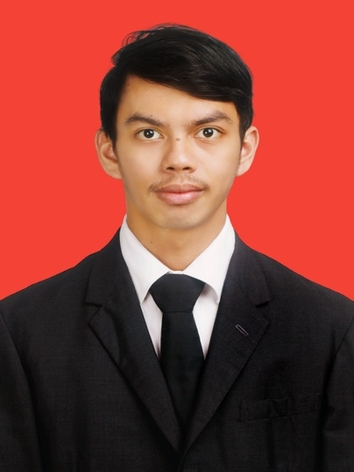
\includegraphics[height=0.2\textheight]{./ubah/3-Pas_Foto_dhani.jpg}
	\end{center}
%*********************************
\section*{Identitas Diri}
\begin{tabular}{p{3cm}cp{9cm}}
	%Masukan Identitas Disini.............
	Nama  		  & :&
		Ahmad Ramadhani \\
	Tempat Lahir  & :&
		Blitar\\
	Tanggal Lahir &:& 
		20 Desember 1998\\
	Alamat        &:& 
	Jalan Klayatan 3 Gang Teratai No. 16C RT 05 RW 02, Kelurahan Bandungrejosari, Kecamatan Sukun, Kota Malang.\\
	Email   &:&
		 ahmadramadhani2098@gmail.com\\
\end{tabular}

\section*{Riwayat Pendidikan}
\begin{tabular}{p{3cm}cp{9cm}}
	2022-Sekarang  	& :&
		Program Magister (S2), Bidang Jaringan Cerdas
		Multimedia (JCM), Departemen Teknik Elektro,
		Fakultas Teknologi Elektro dan Informatika Cerdas, Institut Teknologi Sepuluh Nopember\\
	&&\\
	2017-2021  & :&
		Program Sarjana (S1), Program Studi Pendidikan Teknik Informatika, Departemen Teknik  Elektro dan Informatika, Fakultas Teknik, Universitas Negeri Malang\\
%	&&\\
%	2014-2017  & :&
%		Program Sarjana (S1), Departemen Teknik  Elektro, Fakultas Teknologi Elektro dan Informatika Cerdas, Institut Teknologi  Sepuluh Nopember\\
%	&&\\
%	0000-0000  & :&
%		Pendidikan 1\\
%	&&\\
%	0000-0000  & :&
%		Pendidikan 2\\
%	&&\\
%	0000-0000  & :&
%		Pendidikan 3\\
\end{tabular}


\section*{Daftar Publikasi}

\begin{enumerate}
	\item A. Ramadhani, I. K. Eddy Purnama, E. Mulyanto Yuniarno and J.
	Nugroho, ”Thrombus 
	Segmentation in Ultrasound Deep Vein 
	Thrombosis (DVT) Images using 
	VGG16 and UNet based on Denoising 
	Filters,” 2023 3rd International 
	Biomedical Instrumentation and 
	Technology Conference (IBITeC) 
	2023. Universitas Islam Indonesia, 
	Yogyakarta.
	\item . S. Batan, E. M. Yuniarno, M. H. Purnomo and A. Ramadhani, "Calorie Burn Estimator on Stationary Bike using Human Body Pose Detector," 2023 International Seminar on Intelligent Technology and Its Applications (ISITIA), Surabaya, Indonesia, 2023, pp. 125-129, doi: 10.1109/ISITIA59021.2023.10221128.
	\item I. K. Sari, H. A. Rosyid, T. Prianto, S. Sanjaya and A. Ramadhani, "Non-Intrusive Laboratory Attendance Confirmation via Object Detection using YOLO," 2021 7th International Conference on Electrical, Electronics and Information Engineering (ICEEIE), Malang, Indonesia, 2021, pp. 426-430, doi: 10.1109/ICEEIE52663.2021.9616940.
	
	
%\end{enumerate}
%
%\section*{Riwayat Penelitian}
%\begin{enumerate}
%	\item \lipsum[3]
%	\item \lipsum[3]
%	\item Penelitian Ke Tiga 
%	\item Penelitian Ke Empat 
%\end{enumerate}
%\section*{Riwayat Lainnya}
%
%\lipsum[1]
\cleardoublepage}


\newcommand{\DaftarPustaka}{%\\renewcommand\bibname{Daftar Pustaka}
%\\addcontentsline{toc}{chapter}{\bibname}
%\\titlespacing*{\chapter}{0pt}{0ex}{5ex}
%\\appendix
%\%\bibliographystyle{apalike}
%\%\bibliographystyle{ieetr}
%\%\bibliographystyle{IEEEtranN}
%\\bibliographystyle{plainnat}
%\\bibliography{./ubah/pustaka}
%\\cleardoublepage
\renewcommand\bibname{Daftar Pustaka}
\addcontentsline{toc}{chapter}{\bibname}
\titlespacing*{\chapter}{0pt}{0ex}{5ex}
\appendix
%\bibliographystyle{IEEEtranN}
\bibliographystyle{IEEEtran}
\bibliography{IEEEabrv,./ubah/pustaka}
%\bibliography{pustaka}
\cleardoublepage}

\tolerance=9999
\emergencystretch=10pt
\hyphenpenalty=10000
\exhyphenpenalty=100



%************************************
% 1. JENIS BUKU
%    Pilih Salah Satu 
%************************************
%     \ProposalDisertasi
%     \ProposalTesis 
     \Tesis{Magister Teknik (MT)}
%\Disertasi{Doktor (Dr)}
%***************************

%\ProposalDisertasi
%\ProposalTesis 
%\Tesis{Magister Teknik (MT)}
%\Disertasi{Doktor (Dr)}


%*******************************
%2.  Tulislah Kode Yang Sesuai 
%*******************************
%\Kode{DISERTASI - EE186601}
\Kode{TESIS - EE235401}
%\Kode{Proposal Tesis}
%\Kode{Proposal Disertasi}
%*******************************

%*******************************
%  3. Judul Proposal, Tesis atau 
%     Disertasi 
%     dipilih Salah Satu 
%-------------------------------
% Tulislah Judul Dalam Bahasa Indonesia
\Judul{SEGMENTASI GUMPALAN DARAH VENA PADA CITRA ULTRASOUND MENGGUNAKAN U-NET}
% Tulislah Judul Dalam Bahasa Inggris
\JudulEng{THROMBUS SEGMENTATION IN ULTRASOUND IMAGE USING U-NET}
%************************************
% 4. Identitas Mahasiswa
% Format :\Mahasiswa{Nama}{Nrp}
%------------------------------------
\Mahasiswa{Ahmad Ramadhani}{6022221001}
%************************************
% 5. Waktu Dan Ruang Ujian
%------------------------------------
%Tanggal Ujian 
\TanggalUjian{11 Januari 2024}
% Perioda wisuda  
\PeriodeWisuda{-} 
%Hari ujian dan Tempat Ujian 
\HariUjian{Kamis}
\TempatUjian{Ruang B211}


%************************************
%6. Identitas Pembimbing 
%   Maximal Tiga Pembimbing
%   Format : \PembimbingXXX{Nama}{Nip}
%-----------------------------------
%\scalebox{.95}[1.0]{xxx}
\PembimbingSatu{Prof. Dr. I Ketut Eddy Purnama, S.T., M.T.}{196907301995121001}
\PembimbingDua{Dr. Eko Mulyanto Yuniarno, S.T., M.T.}{196806011995121009}
%\PembimbingTiga{Dr. Eko Mulyanto Yuniarno,ST. MT.}{132135221}

%************************************
% 7. Identitas Penguji 
%     Maximal 4 penguji
%     Format : \PengujiXXX{Nama}{Nip}
%-------------------------
\PengujiSatu{Dr. Arief Kurniawan, S.T., M.T.}{197409072002121001}
\PengujiDua{Dr. Eko Mulyanto Yuniarno, S.T., M.T.}{196806011995121009}
\PengujiTiga{Dr. Supeno Mardi Susiki Nugroho, S.T., M.T.}{197003131995121001}
% \PengujiTiga{Dr. I Ketut Eddy Purnama, S.T., M.T.}{196907301995121001}
% \PengujiEmpat{Dr. Eko Mulyanto Yuniarno, S.T., M.T.}{196806011995121009}
%\PengujiTiga{Dr.Eko Mulyanto Yuniarno}{196806011995121009}
%\PengujiEmpat{Dr.Eko Mulyanto Yuniarno}{132135221}

%************************************
% 8. Identitas Fakultas ------------------------------------
\Fakultas{Fakultas Teknologi Elektro Dan Informatika Cerdas}
\BeltFakultas{BeltFte}
%************************************
% 9. Identitas Departement
%-----------------------------------
\Departemen{Teknik Elektro}

\KaDep{Dedet Candra Riawan, ST., M.Eng., Ph.D}{197311192000031001}
%***********************************
% 10. Footer Identitas Program Studi 
%  Pada Cover
%----------------------------------
\CoverFooter{\normalsize
PROGRAM MAGISTER\\
	DEPARTEMEN TEKNIK ELEKTRO\\
	FAKULTAS TEKNOLOGI ELEKTRO DAN INFORMATIKA CERDAS\\
	INSTITUT TEKNOLOGI SEPULUH NOPEMBER\\
	SURABAYA\\
	2024}

%**********************************
%File Penting Yang Dapat di Edit:
%**********************************
%Abstrak :
%        ->\ubah\abstrak.tex
%Abstrak Bhs Inggris :
%        ->\ubah\abstrakEng.tex
%Kata Penggantar :
%        ->\ubah\pengantar.tex 
%Nomenklatur :
%        ->\ubah\Nomenklatur.tex
%Database Daftar Pustaka
%        ->\ubah\pustaka.bib
%DaftarRiwayatHidup 
%        ->\ubah\DaftarRiwayatHidup.tex
%----------------------------------
%**********************************
%Dokumen Utama
%----------------------------------
\begin{document}
%%%%%%%%%%%%%%%%%%%%%%%%%%%%%%%%%%%%%%%%%%%%
% FILE INI JANGAN DI UBAH ATAU MODIFIKASI
%%%%%%%%%%%%%%%%%%%%%%%%%%%%%%%%%%%%%%%%%%%%
\normalsize
\pagenumbering{roman}
\singlespacing
 \hyphenpenalty=1000
\tolerance=1000
\emergencystretch=2.5em
% Cover
%\addcontentsline{toc}{chapter}{Cover}
\begin{FontCover}
	\sffamily	
\thispagestyle{empty}
\begin{figure} [!t]
	
\includegraphics[keepaspectratio=true,scale=1,left]{lib/LogoITS.png}
	\caption*{}
	\label{fig:LogoITS}
\end{figure}
\vspace{1ex}
%\noindent\makebox[\linewidth]{\rule{\paperwidth}{10pt}}
\makebox[\linewidth]{\includegraphics[keepaspectratio=true,width=\paperwidth]{lib/\bbelt}}
\vspace{10ex}
\justify
\textbf{\Kodekk}
\vspace{1ex}
\justify
\Large
\begin{spacing}{1}
%Masukan Judul Tesis Disini
\flushleft
\textbf{\JdTesis}
\end{spacing}
\normalsize
\vfill
\justify

%\begin{spacing}{1}
\large
\MakeUppercase{\NamaMahasiswa}\\
NRP  \uppercase{\NrpMahasiswa}
\vspace{2ex}
\justify
\normalsize

\ifthenelse{\boolean{bMaster}}{\textbf{DOSEN PEMBIMBING}}{\textbf{PROMOTOR}}\\
\PbSatu\\
\ifthenelse{\boolean{PembimbingDua}}{\ifthenelse{\boolean{bMaster}}{}{\\\textbf{Co.PROMOTOR\\}}}{}
\ifthenelse{\boolean{PembimbingDua}}{\PbDua\\}{}
\ifthenelse{\boolean{PembimbingTiga}}{\PbTiga\\}{}
 
\vfill
\justify
\bdk
\vspace{1ex}
%\rmfamily
\normalfont
\end{FontCover}
\newpage
\cleardoublepage
% Lembar pengesahan
\addcontentsline{toc}{chapter}{LEMBAR PENGESAHAN}
     
\ifthenelse{\boolean{bThesis}}
{ \AddToShipoutPicture*{\BackgroundIm}
\begin{center}

\Large\textbf{\pPengesahan}
%\Large\textbf{PROPOSAL TESIS}
\end{center}
\begin{center}
\tsss\\
\textbf{\ggGelar}\\
di\\
\textbf{Institut Teknologi Sepuluh Nopember}\\
\vspace{1ex}
Oleh:\\
\textbf{\NamaMahasiswa}\\ 
\textbf{NRP:\NrpMahasiswa}\\ 
\vspace{1ex}
Tanggal Ujian :\TglUjian\\
Periode Wisuda : \PerWisuda\\
\vspace{1ex}
\end{center}
\begin{center}
Disetujui oleh:\\
\textbf{Pembimbing}:
\end{center}
\begin{enumerate}
\item \PbSatu \hfill ...............................\\
NIP:\NipPbSatu \vfill
\ifthenelse{\boolean{PembimbingDua}}{\item \PbDua\hfill ...............................\\
NIP:\NipPbDua}\vfill
\ifthenelse{\boolean{PembimbingTiga}}{\item \PbTiga \hfill ...............................\\
	NIP:\NipPbTiga}{}
\end{enumerate}	
\begin{center}
	\textbf{Penguji}:
\end{center}
\begin{enumerate}
	\item \PjSatu \hfill ...............................\\
	NIP:\NipPjSatu
	\vfill
	\item \PjDua \hfill ...............................\\
	NIP:\NipPjDua\vfill
\ifthenelse{\boolean{PengujiTiga}}{
	\item \PjTiga \hfill ...............................\\NIP:\NipPjTiga\vfill}{}
\ifthenelse{\boolean{PengujiEmpat}}{
	\item \PjEmpat \hfill ...............................\\ NIP:\NipPjEmpat\vfill}{}
\end{enumerate}	
\vfill
\begin{center}
	Kepala Departemen \Dep \\
	 \fak\\
	\vspace{9ex}
	\underline{\NmKaDep}\\
	Nip:\NipKaDep
\end{center}
\newpage
}
{
\begin{center}
\textbf{LEMBAR PENGESAHAN\\
	\prop}\\    
\end{center}
\vspace{5ex}
\begin{tabular}{p{2cm} c p{8cm}}
Judul&:&\JdTesis\\
Oleh &:&\NamaMahasiswa\\
Nrp&:&\NrpMahasiswa
\end{tabular}
\vspace{5ex}
\begin{center}
\textbf{Telah Diseminarkan  Pada}
\end{center}
\begin{tabular}{p{2cm} c p{8cm}}
Hari &:&\bHariUjian\\
Tanggal &:&\TglUjian\\
Tempat&:&\bTempatUjian
\end{tabular}
\vspace{5ex}
%\scalebox{.95}[1.0]{\PjSatu}

\begin{tabular}{p{8cm} p{8cm} }
\textbf{Penguji}& \textbf{Calon Pembimbing}\\
\vspace{8ex}\hspace{-10ex}1. \PjSatu&
\vspace{8ex}\hspace{-8ex}1. \PbSatu \\
\hspace{-7ex}Nip :\NipPjSatu&
\hspace{-5ex}Nip :\NipPbSatu\\
\vspace{8ex}\hspace{-10ex}2. \PjDua&
\ifthenelse{\boolean{PembimbingDua}}
{\vspace{8ex}\hspace{-8ex}2. \PbDua}{} \\
\hspace{-7ex}Nip :\NipPjDua&
\ifthenelse{\boolean{PembimbingDua}}
{\hspace{-5ex}Nip :\NipPbDua}{}\\
\ifthenelse{\boolean{PengujiTiga}}
{\vspace{8ex}\hspace{-10ex}3. \PjTiga}{}&
\ifthenelse{\boolean{PembimbingTiga}}
{\vspace{8ex}\hspace{-8ex}3. \PbTiga}{} \\
\ifthenelse{\boolean{PengujiTiga}}
{\hspace{-7ex}Nip :\NipPjTiga}{}&
\ifthenelse{\boolean{PembimbingTiga}}
{\hspace{-5ex}Nip :\NipPbTiga}{}\\


\ifthenelse{\boolean{PengujiEmpat}}
{\vspace{8ex}\hspace{-10ex}4. \PjTiga}{}& \\
\ifthenelse{\boolean{PengujiEmpat}}
{\hspace{-7ex}Nip :\NipPjEmpat}{}&\\
\end{tabular}
\newpage
}
\cleardoublepage

\ifthenelse{\boolean{bThesis}}
{
	\ifthenelse{\boolean{bMaster}}
	{
\chapter*{PERNYATAAN KEASLIAN TESIS}
\addcontentsline{toc}{chapter}{PERNYATAAN KEASLIAN TESIS}


\begin{spacing}{1.5}
	
	Dengan ini saya menyatakan bahwa isi keseluruhan Tesis saya dengan judul \textbf{\JdTesis} adalah benar-benar hasil karya intelektual mandiri, diselesaikan tanpa menggunakan bahan-bahan yang tidak diijinkan dan bukan merupakan karya pihak lain yang saya akui sebagai karya sendiri.
	
	Semua referensi yang dikutip maupun dirujuk telah ditulis secara lengkap pada daftar pustaka. Apabila ternyata pernyataan ini tidak benar, saya bersedia menerima sanksi sesuai peraturan yang berlaku.
	
	\hspace{30ex}Surabaya \today
	
	\vspace{10ex}
	
	\hspace{35ex}\underline{\NamaMahasiswa}
	
	\hspace{35ex}Nrp :\NrpMahasiswa
	
\end{spacing}
\cleardoublepage

}
{
	
	\chapter*{PERNYATAAN KEASLIAN DISERTASI}
	\addcontentsline{toc}{chapter}{PERNYATAAN KEASLIAN DISERTASI}
	
	\begin{spacing}{1.5}
		
		Dengan ini saya menyatakan bahwa isi keseluruhan Disertasi  saya dengan judul \textbf{\JdTesis} adalah benar-benar hasil karya intelektual mandiri, diselesaikan tanpa menggunakan bahan-bahan yang tidak diijinkan dan bukan merupakan karya pihak lain yang saya akui sebagai karya sendiri.
	
	Semua referensi yang dikutip maupun dirujuk telah ditulis secara lengkap pada daftar pustaka. Apabila ternyata pernyataan ini tidak benar, saya bersedia menerima sanksi sesuai peraturan yang berlaku.
	
	\hspace{30ex}Surabaya \today
	
	\vspace{10ex}
	
	\hspace{35ex}\underline{\NamaMahasiswa}
	
	\hspace{35ex}Nrp :\NrpMahasiswa
	
\end{spacing}
\cleardoublepage
}
}{}




% Kata pengantar
\newpage

\addcontentsline{toc}{chapter}{KATA PENGANTAR}
\begin{center}
\Large\textbf{Kata Pengantar}
\end{center}
\vspace{2ex}
%Tulis kata pengantar di sini
Puji dan syukur kehadirat Allah SWT atas segala limpahan berkah, rahmat, serta hidayah-Nya, penulis  dapat menyelesaikan laporan ini dengan judul SEGMENTASI GUMPALAN DARAH VENA PADA CITRA ULTRASOUND MENGGUNAKAN U-NET.

Pada penulisan buku tesis ini, penulis memiliki banyak kekurangan dan keterbatasan sehingga proses penyusunan buku tesis ini tidak lepas dari bantuan, dukungan, dan bimbingan dari berbagai pihak. Oleh karena itu, dengan hormat, penulis mengucapkan terima kasih kepada:

\begin{enumerate}
	\item Prof. Dr. I Ketut Eddy Purnama, S.T., M.T. dan Dr. Eko Mulyanto Yuniarno, S.T., M.T. yang telah mengarahkan, memberikan semangat, saran, dan masukan dalam penyusunan buku tesis.
	\item Dr. Eko Mulyanto Yuniarno, S.T., M.T. selaku koordinator bidang keahlian Jaringan Cerdas Multimedia.
	\item Dewan penguji yang telah memberikan masukan dan arahan dalam tesis ini.
	\item Orang tua dan keluarga yang selalu memberikan bantuan dalam bentuk moral, material, dan doa kepada penulis.
	\item Teman - teman seperjuangan JCM yang telah memberikan dukungan dalam pengerjaan tesis ini.
	\item Teman - teman Lab Visi Komputer (B300) yang memberi semangat, kritik, dan saran, serta dukungan dalam penyelesaian buku tesis ini.
	\item Semua pihak yang telah membantu dalam proses pengerjaan buku tesis ini.
\end{enumerate}

 \vspace{1ex}
Dalam penyusunan buku tesis ini, penulis menyadari bahwa masih terdapat kekurangan dalam segi penulisan maupun isi dari tesis. Oleh karena itu, kritik dan saran yang membangun sangat diharapkan oleh penulis
	\vspace{26pt}
	\begin{flushright}
		\begin{tabular}[b]{c}
			Surabaya, 21 Desember 2023
			\\
			\\
			\\
			Penulis
		\end{tabular}
	\end{flushright}

\cleardoublepage
\newpage
% Abstrak
\begin{spacing}{1}
\begin{center}
		\large\textbf{\JdTesis}
	\end{center}
	\normalsize
	\begin{adjustwidth}{-0.2cm}{}
		\ifthenelse{\boolean{bMaster}}{
		
		\begin{tabular}{lcp{0.9\linewidth}}
		Nama Mahasiswa &:& \NamaMahasiswa\\
			NRP &:&\NrpMahasiswa\\
			Pembimbing &:& 1. \PbSatu\\
			\ifthenelse{\boolean{PembimbingDua}}{& & 2. \PbDua\\}{}
			
			\ifthenelse{\boolean{PembimbingTiga}}{& & 3. \PbTiga\\}{}
			
			
			
		\end{tabular}
	}{
	\begin{tabular}{lcp{0.7\linewidth}}
		Nama Mahasiswa &:& \NamaMahasiswa\\
		NRP &:&\NrpMahasiswa\\
		Promotor &:&  \PbSatu\\
		\ifthenelse{\boolean{PembimbingTiga}}{
		\ifthenelse{\boolean{PembimbingDua}}{Co. Promotor&: & 1. \PbDua\\}{}
		\ifthenelse{\boolean{PembimbingTiga}}{& & 2. \PbTiga\\}{}
	}
{
	\ifthenelse{\boolean{PembimbingDua}}{\hspace{5ex}Co. Promotor&: & \PbDua\\}{}
	
}
	\end{tabular}

}

	
	\end{adjustwidth}
	\vspace{2ex}
	\begin{center}
		\Large\textbf{ABSTRAK}
	\end{center}
	\vspace{1ex}	
%Tulis Abstrak disini
\textit{Deep Vein Thrombosis} (DVT) merupakan sebuah penyakit yang diakibatkan adanya pembentukan thrombus pada pembuluh darah vena dalam. Thrombus ini dapat mengganggu aliran darah normal dan menyebabkan masalah serius apabila tidak diobati. Dataset yang digunakan dalam penelitian ini berupa citra 2D \textit{ultrasound thrombus} 5 pasien penderita DVT dan citra \textit{thrombus} dan pembuluh darah \textit{phantom} balon panjang. Diagnosis thrombus apabila dilakukan secara manual memerlukan waktu yang tidak sebentar serta analisis akurasi pembacaan citra \textit{thrombus} bergantung pada dokter spesialis. Oleh karena itu, diperlukan adanya diagnosis \textit{thrombus} untuk penderita DVT secara otomatis guna mempersingkat waktu serta meningkatkan performa analisis akurasi pembacaan citra \textit{thrombus}. Penelitian ini mengusulkan segmentasi 2D dan 3D \textit{thrombus} pada citra \textit{ultrasound} \textit{phantom} balon panjang menggunakan model segmentasi U-Net. Penelitian ini berhasil melakukan segmentasi gumpalan darah vena pada citra \textit{ultrasound} menggunakan U-Net 3D. Berdasarkan hasil segmentasimodel segmentasi U-Net 3D mendapat nilai \textit{accuracy} sebesar 99,1078\% dan nilai \textit{loss} sebesar 0,0208. Berdasarkan perhitungan evaluasi metrik untuk perhitungan antara hasil citra prediksi dan groundtruth dengan menggunakan IoU, \textit{dice coefficient}, dan \textit{hausdorff distance}, citra 3D \textit{ultrasound} \textit{thrombus} dan pembuluh darah mendapat nilai \textit{mean} IoU sebesar 0,8105, \textit{mean dice coefficient} sebesar 0,8953, dan \textit{mean hausdorff distance} sebesar 3,25. Pada segmentasi 2D citra \textit{ultrasound} \textit{thrombus} dan pembuluh darah \textit{phantom} balon panjang, penggunaan \textit{encoder} \textit{pre-trained VGG16} pada model U-Net 2D dapat meningkatkan kinerja model untuk segmentasi area \textit{thrombus}. Penerapan peningkatan kualitas citra dengan filter \textit{gaussian} dan filter \textit{median} memberikan pengaruh dalam peningkatan performa segmentasi 2D. \\

%Tulis Kata Kunci disini
\vspace{2ex}
\textbf{Kata kunci }: \textit{Deep Vein Thrombosis},  Citra \textit{Ultrasound}, segmentasi, \textit{pre-trained} VGG16 and UNet, filter \textit{denoising}
	
\end{spacing}
\cleardoublepage
\ifthenelse{\boolean{JudulTesisEng}}
{
	\begin{spacing}{1}
\begin{center}
		\large\textbf{\JdTesisEng}
	\end{center}
	\normalsize
	\begin{adjustwidth}{-0.2cm}{}
		\begin{tabular}{lcp{0.9\linewidth}}
		By &:& \NamaMahasiswa\\
			Student Identity Number &:&\NrpMahasiswa\\
			Supervisor &:& 1. \PbSatu\\
			\ifthenelse{\boolean{PembimbingDua}}{& & 2. \PbDua\\}{}
			\ifthenelse{\boolean{PembimbingTiga}}{& & 3. \PbTiga\\}{}
		\end{tabular}
	\end{adjustwidth}
	\vspace{2ex}
	
	\begin{center}
		\Large\textbf{ABSTRACT}
	\end{center}
	\vspace{1ex}	
%Tulis Abstrak disini
Deep Vein Thrombosis (DVT) is a disease that occurs when a thrombus forms within the deep veins. This thrombus can disrupt normal blood flow and lead to severe issues if left untreated. The dataset used in this research consists of 2D ultrasound images of thrombus from 5 patients with DVT. Manual thrombus diagnosis requires a considerable amount of time, and the accuracy of thrombus image analysis relies on specialized doctors. Hence, an automatic thrombus diagnosis is needed for DVT patients to shorten the time and enhance the accuracy of thrombus image analysis. This research proposes thrombus segmentation in ultrasound images using pre-trained VGG16 and UNet model based on denoising filters. The encoder for the UNet model in this segmentation model is a pre-trained VGG16 model. In this study, five denoising filters are utilized.Based on the conducted experiments, the Gaussian filter yielded the most optimal results for thrombus segmentation with an accuracy of 99.166\% and a loss value of 0.0269 for the UNet model. Furthermore, the pre-trained VGG16 and UNet model's accuracy was 99.222\%, and the loss value was 0.284. Thrombus prediction tests using the UNet model resulted in a mean IoU of 77.087\%, a mean Dice coefficient of 0.8608, and a mean Hausdorff distance of 3.44. Meanwhile, thrombus prediction tests using the pre-trained VGG16 and UNet model produced a mean IoU of 88.298\%, a mean Dice coefficient of 0.8784, and a mean Hausdorff distance of 3.07. As a result, utilizing VGG16 as the encoder in the UNet architecture may enhance accuracy when segmenting. \\

%Tulis Kata Kunci disini
\vspace{2ex}
\textbf{Keyword}: Deep Vein Thrombosis,  Ultrasound Image, Segmentation, Pre-trained VGG16 and UNet, Denoising Filter
\end{spacing}
}{}
\cleardoublepage

% Daftar isi
\renewcommand*\contentsname{DAFTAR ISI}
\titlespacing*{\chapter}{0pt}{0ex}{0ex}
\tableofcontents
\cleardoublepage
% Daftar gambar
\renewcommand*\listfigurename{DAFTAR GAMBAR}
\addcontentsline{toc}{chapter}{\listfigurename}
\titlespacing*{\chapter}{0pt}{0ex}{0ex}
\listoffigures
\cleardoublepage
% Daftar tabel
\renewcommand*\listtablename{DAFTAR TABEL}
\addcontentsline{toc}{chapter}{\listtablename}
\titlespacing*{\chapter}{0pt}{0ex}{0ex}
\listoftables
\cleardoublepage
% Nomenklatur
\addcontentsline{toc}{chapter}{NOMENKLATUR} % kata pengantar
\begin{center}
\Large\textbf{NOMENKLATUR}
\end{center}
\vspace{1ex}
\begin{conditions}
%		M &	Markov \textit{Decision Process}.\\
%		S &	\textit{State}.\\
%		\alpha& Learning Rate
		$_{P}^{T}T$ & Transformasi dari marker pada probe ultrasound ke pusat koordinat sistem kamera \textit{optictrack} \\
		$_{U}^{P}T$ & merupakan transformasi dari bidang citra \textit{ultrasound} ke marker pada \textit{probe ultrasound} \\
		
\end{conditions}
\newpage

\cleardoublepage

% Bab isi buku
\titleformat{\chapter}[display]{\bfseries\Large}{BAB \centering\thechapter}{0ex}{\vspace{0ex}\centering}[\vspace{0ex}]
\titleformat{\section}{\bfseries\large}{\MakeUppercase{\thesection}}{1ex}{}
\titleformat{\subsection}{\bfseries\large}{\MakeUppercase{\thesubsection}}{1ex}{}
\titleformat{\subsubsection}{\bfseries\large}{\MakeUppercase{\thesubsubsection}}{1ex}{}
\titlespacing*{\chapter}{0pt}{-4ex}{0pt}
\titlespacing{\section}{0pt}{0pt}{0pt}
\titlespacing{\subsection}{0pt}{0pt}{0pt}
\titlespacing{\subsubsection}{0pt}{0pt}{0pt}
% Indent paragraph
\setlength{\parindent}{0.8cm}
\begin{spacing}{1.5}
	
\begin{spacing}{1.2}
  \chapter{PENDAHULUAN}
\end{spacing}


\pagenumbering{arabic}
\vspace{4ex}

\section{Latar Belakang}
\textit{Deep Vein Thrombosis} (DVT) merupakan sebuah penyakit yang diakibatkan adanya pembentukan gumpalan darah (\textit{thrombus}) pada pembuluh darah vena dalam. Gumpalan darah tersebut dapat menimbulkan penyumbatan pada pembuluh darah di paru – paru sehingga berpotensi menyebabkan kondisi yang serius sepeti \textit{Pulmonory Embolism} (PE)\cite{arta1}. Penanganan medis pada kasus DVT secara konvensional dilakukan dengan cara penyedotan thrombus yang terdeteksi dalam pembuluh darah vena. Kegiatan penyedotan tersebut biasa disebut dengan aspirasi.

Pemantauan proses aspirasi menggunakan angiografi berbasis X-Ray. Pemantauan ini dilakukan sebelum operasi dan sesudah operasi. Angiografi berbasis X-Ray beresiko menimbulkan paparan radiasi kepada pasien maupun tenaga medis. Angiografi hanya dapat menampilkan citra 2D sehingga objek yang berbentuk volume tidak dapat divisualkan\cite{made2020}. Modalitas \textit{ultrasound} (USG) diusulkan karena USG tidak memiliki resiko penyebaran paparan radiasi jika dibandingkan dengan modalitas yang digunakan sekarang yaitu X-Ray. Selain itu, proses pencitraan modalitas menggunakan USG memungkinkan untuk mendapatkan citra 2D.

Kelemahan pencitraan DVT menggunakan modalitas USG yaitu citra yang dihasilkan dari proses pencitraan USG cenderung sulit untuk dianalisis dan memiliki banyak noise. Perbedaan citra hasil pencitraan USG bisa mempengaruhi proses diagnosis dokter sehingga memungkinkan terjadinya kesalahan dalam memberikan informasi letak posisi gumpalan darah. Oleh karena itu, perlu adanya pengolahan citra hasil pencitraan menggunakan USG agar dapat divisualisasikan guna mengetahui informasi – informasi penting yang terkait dengan kasus DVT seperti volume dari pembuluh darah vena ataupun gumpalan darah.

Metode deteksi gumpalan darah konvensional biasanya mengadopsi algoritma pemrosesan gambar, seperti peningkatan kualitas citra gambar, segmentasi, dan pengklasifikasian. Namun, untuk mendapatkan hasil yang akurat, metode – metode konvensional ini masih memerlukan peningkatan yang lebih kompleks. Belakangan ini, metode \textit{deep learning} telah diperkenalkan untuk analisis gambar medis untuk berbagai masalah dengan mendapatkan hasil dengan akurasi yang sangat baik. \textit{Convolutional Neural Network} (CNN) telah menarik perhatian banyak peneliti saat ini [3]. Dikarenakan model CNN dapat dilatih dan dibelajari fitur – fitur sesuai dengan keinginan peneliti.

Penelitian yang telah dilakukan oleh Sunarya, dkk (2020)\cite{made2020} menitikberatkan pada pengembangan visualisasi rekonstruksi citra 3D pembuluh darah arteri karotis yang berasal dari citra \textit{B-Mode ultrasound}. Segmentasi pada penelitian ini masih menggunakan pendekatan \textit{matching template features}. Adapun kekurangan dari metode \textit{matching ellipses features} adalah citra yang dihasilkan hanya sebatas \textit{binary semantic segmentation} serta hasil ekstraksi tepi (outer) pembuluh darah tidak berdasarkan bentuk yang sesungguhnya.

Penelitian yang telah dilakukan oleh Hernanda, dkk (2022)\cite{arta1} memperbaiki kekurangan yang ada pada penelitian Sunarya (2020)\cite{made2020} berhasil mendapatkan hasil ekstraksi tepi (\textit{outer}) yang sesuai dengan bentuk pembuluh darah sesungguhnya dari hasil segmentasi citra 2D menggunakan model U-Net. Penelitian ini juga dapat memvisualisasikan rekonstruksi 3D dari hasil segmentasi \textit{semantic} citra 2D uSG pembuluh darah vena menggunakan model \textit{deep learning} U-Net. Namun kekurangan dari penelitian ini adalah hanya sebatas \textit{binary class segmentation} sehingga belum dapat membedakan mana yang termasuk pembuluh darah ataupun gumpalan darah. Dari kekurangan tersebut, maka perlu adanya pengembangan metode untuk \textit{multiclass segmentation} yang lebih efisien guna mendapatkan area gumpalan darah vena secara akurat. Oleh karena itu pada penelitian ini akan dilakukan segmentasi dari citra 2D gumpalan darah pada pembulah darah vena menggunakan arsitektur \textit{deep learning} U-Net. Proses segmentasi gumpalan darah (\textit{thrombus}) menggunakan model U-Net sudah dilakukan oleh Mojtahedi (2022) \cite{mojtahedi2022fully} untuk mencari area dari \textit{thrombus} pada arteri selebral arterior pada penderita \textit{stroke}. Namun pada penelitian ini masih belum optimal karena jumlah data \textit{training} hanya 208 citra serta kurangnya variasi data yang digunakan.



% Sebagian besar implementasi model CNN pada deteksi terkait darah hanya terbatas pada model 2D CNN. Namun 2D CNN tidak dapat diimplementasikan pada dataset 3D. Beberapa jenis model 2D CNN mencoba untuk memperkenalkan sudut pandang multi tampilan atau fitur 3D yang dikembangkan secara manual. Namun, jenis – jenis CNN 2D ini masih belum sepenuhnya menggali informasi spasial 3D dalam data volumetric. Berbagai jenis CNN 3D diusulkan untuk mengatasi kekurangan dari model CNN 2D.

% Di dalam reduksi False Positive (FP), sangat sedikit model 2D CNN yang sudah diadaptasikan karena memiliki keterbatasan dalam keefektifan dalam membedakan fitur - fitur yang relevan. Oleh karena itu, model 3D CNN secara umum digunakan dalam permasalahan pereduksian FP\cite{reductionBab1Khan}.


  
% Penelitian sebelumnya yang telah dilakukan oleh Hernanda et al (2023) telah berhasil mengembangkan sebuah visualisasi rekonstruksi citra 3D pembuluh darah vena dari citra USG. Metode yang digunakan dalam proses segmentasi yaitu arsitektur deep learning U-Net. 

% Oleh karena itu pada penelitian ini akan dilakukan segmentasi dari citra 2D gumpalan darah pada pembulah darah vena menggunakan arsitektur \textit{deep learning} V-Net.

\section{Rumusan Masalah}
Berdasarkan latar belakang yang dijelaskan sebelumnya, maka dapat dirumuskan permasalahan yaitu sistem segmentasi peredaran darah manusia pada penelitian sebelumnya belum dapat membedakan mana yang termasuk bentuk gumpalan darah. 
\section{Tujuan}
Tujuan dari penelitian ini adalah untuk melakukan segmentasi 2D dan 3D gumpalan darah pada pembuluh darah vena dengan menggunakan citra 2D dan 3D \textit{ultrasound.} Sistem segmentasi gumpalan darah ini nantinya sebagai dasar untuk perhitungan volumetric gumpalan darah.

%\cite{Koza1996}
%\begin{enumerate}
%	\item Tujuan Pertama
%	\item Tujuan Kedua
%\end{enumerate}
%\section{Batasan Masalah}
%Tutorial ini dibatasi pada penggunaan Latex untuk penulisan tesis. 
\section{Manfaat}
Manfaat yang diperoleh dari penelitian ini mengembangkan sistem segmentasi gumpalan darah pada pembuluh darah vena dari citra 2D dan 3D USG. Dengan adanya segmentasi 2D dan 3D gumpalan darah pada pembuluh darah vena dapat menjadi dasar pengembangan selanjutnya perhitungan volumetric gumpalan darah. 
%\subtem section{Contoh Subseksi }
%\subsubsection{Contoh SubSub Seksi}
%
%\begin{equation}
%y=cos(\alpha x)
%\end{equation}

	\cleardoublepage
	\chapter{KAJIAN PUSTAKA}


\section*{ }
Demi mendukung penelitian ini, dibutuhkan beberapa teori penunjang sebagai bahan acuan dan referensi. Dengan demikian penelitian ini menjadi lebih terarah. 
\vspace{1ex}

\section{Gumpalan Darah Vena}

Gumpalan darah atau yang biasa disebut dengan \textit{thrombus} merupakan massa padat yang terbentuk dari pembekuan darah di dalam pembuluh darah\cite{ashorobi2022thrombosis}. Adanya gumpalan darah ini yang dapat memicu terkena penyakit \textit{ Deep Vein Thrombosis} (DVT). DVT merupakan sebuah kondisi dimana adanya pembekuan darah pada daerah vena bagian dalam. Sebagian besar kasus, DVT terbentuk pada pembuluh darah pada area paha atau betis, tetapi tidak menutup kemungkinan terbentuk pada pembuluh darah pada area yang lain. 

Penyebab DVT mencakup tiga faktor utama yaitu (1) stasis vena (\textit{venous stasis}); (2) gangguan vaskular (\textit{vascular injury}); serta (3) hiperkoagulabilitas (\textit{hypercoagulability})\cite{Jonathan2017}. Stasis vena terjadi ketika aliran darah terhambat, seringkali karena kurangnya aktivitas fisik, seperti pasien yang terbaring lama atau dalam perjalanan jauh. Gangguan vaskular dapat disebabkan oleh operasi, trauma, atau inflamasi pada dinding vena. Hiperkoagulabilitas merupakan kondisi dimana darah lebih mudah untuk membeku yang disebabkan oleh beberapa faktor seperti kondisi genetik, kehamilan, atau kanker.   

Penyakit DVT harus segera didiagnosa dan ditangani secara cepat. Seringkali gejala DVT munculnya tidak secara spesifik dan bisa tidak terdeteksi. Namun, gejala umum yang muncul dari penyakit DVT dapat berupa (1) nyeri; (2) bengkak - bengkak; (3) pembuluh darah membesar di area yang terkena komplikasi jangka panjang DVT yang disebut juga dengan sindrom pascatrombotik yang dapat menyebabkan nyeri, bengkak, sensasi berat, dan kasus yang lebih parah yaitu tumbuh bisul. Berikut ini ilustrasi dari pasien yang terkena DVT yang dapat dilihat pada Gambar\ref{fig:dvtIlustration}.

\begin{figure}[H]
	\centering
	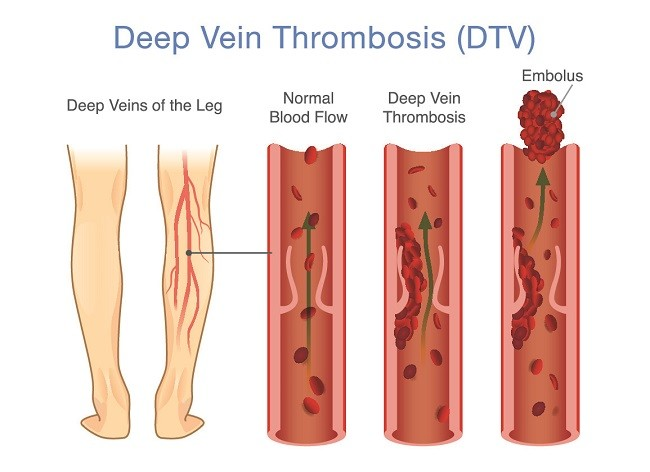
\includegraphics[scale= 0.3]{bab2/deep-vein-thrombosis.jpg}
	\caption{Ilustrasi DVT}
	\label{fig:dvtIlustration}
\end{figure}

%\underline{Menulis Dartar Item}
%\begin{itemize}
%	\item Ini Urutan Pertama. Ini Urutan Pertama. Ini Urutan Pertama. Ini Urutan Pertama. Ini Urutan Pertama. Ini Urutan Pertama. Ini Urutan Pertama. 
%	\item Menulis Item kedua.Menulis Item kedua.Menulis Item kedua.Menulis Item kedua.Menulis Item kedua.Menulis Item kedua.Menulis Item kedua.
%	\item Ini Urutan Ketiga
%\end{itemize}
%
%\underline{Menulis daftar urutan}
%\begin{enumerate}
%	\item Ini Urutan Pertama
%	\item Ini Urutan kedua
%	\begin{enumerate}
%		\item Sub Urutan Pertama
%		\item Sub Urutan Kedua
%	\end{enumerate} 
%	\item Ini Urutan Ketiga
%\end{enumerate}
\section{Citra Ultrasonografi}
Citra \textit{ultrasound} adalah citra medis yang dibuat menggunakan gelombang suara tinggi (\textit{ultrasound}) untuk memvisualisasikan organ tubuh dan struktur di dalamnya\cite{MIT2022}. Citra ini digunakan dalam bidang medis untuk tujuan diagnosis dan pemantauan kondisi kesehatan. Gambar yang dihasilkan oleh citra \textit{ultrasound} (USG) terdiri dari piksel yang mewakili gema (\textit{echo}) yang diterima oleh transduser (\textit{probe}) dan menunjukkan masing-masing bagian organ tubuh\cite{cloutier2021quantitative}. Dengan cara ini, mode ini biasanya menampilkan bagian-bagian tubuh secara rinci. \textit{Probe} yang ditempelkan pada kulit pasien mengirimkan sinyal \textit{ultrasound} ke tubuh pasien, yang kemudian merefleksikan dan menyebar, menghasilkan gema yang digunakan untuk membentuk citra \textit{ultrasound}. 

Pemrosesan citra 2D menggunakan komputer biasa disebut dengan pengolahan citra digital. Citra digital dapat dinyatakan sebagai suatu fungsi dua dimensi f(x,y), dengan x maupun y merupakan posisi koordinat sedangkan f merupakan amplitudo pada posisi(x,y) yang sering dikenal sebagai \textit{grey scale}\cite{Purnomo2010}. Citra digital dapat dibayangkan sebagai suatu matriks yang mana baris dan kolomnya merepresentasikan suatu titik di dalam citra dan nilai elemen matriks tersebut menunjukkan nilai warna pada titik tersebut. Salah satu contoh terdapat citra berukuran 128x128 piksel dengan intensitas beragam pada tiap pikselnya. Setiap pikselnya direpresentasikan secara numerik dengan matriks terdiri dari 128 baris dan 128 kolom. Nilai intensitas atau piksel bentuknya adalah diskrit mulai dari 0 hingga 255, yang mana angka 0 merupakan nilai intensitas paling gelap sedangkan angka 255 merupakan nilai intensitas yang paling terang. 

Adapun pengidentifikasian DVT oleh dokter, pencintraannya menggunakan \textit{ultrasound} jenis \textit{Doppler}. \textit{Ultrasound Doppler} merupakan proses pencitraan menggunakan gelombang suara untuk menunjukkan darah bergerak melalui pembuluh darah\cite{shah2022sonography}. \textit{Ultrasound Doppler} bekerja dengan mengukur gelombang suara yang dipantulkan dari objek bergerak seperti sel darah merah yang biasa disebut dengan efek \textit{Doppler}. Berikut ini hasil pencitraan menggunakan \textit{ultrasound Doppler} yang dapat dilihat pada Gambar \ref{fig:dopler}


\begin{figure}[H]
	\centering
	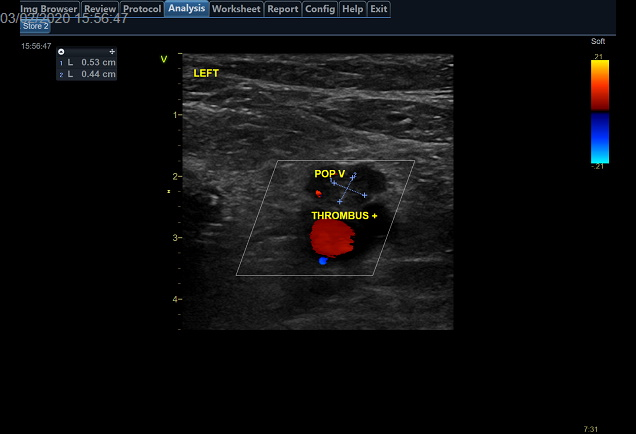
\includegraphics[scale= 0.5]{bab2/yud8Dopler.jpg}
	\caption{Hasil Pencitraan Ultrasound Dopler}
	\label{fig:dopler}
\end{figure}


%\section{Citra Ultrasonografi Tiga Dimensi}
\section{Kalibrasi}
Dalam prosedur kalibrasi menggunakan \textit{probe} \textit{ultrasound}, kami menggunakan sebuah alat yang disebut dengan kotak kalibrasi \textit{double-N}. Proses ini melibatkan beberapa langkah penting untuk memastikan keakuratan alat. Adapun prosedur pertama yaitu merancang kotak kalibrasi \textit{double-N}. Rancangan kotak kalibrasi \textit{double-N} harus sesuai dengan standar yang diperlukan agar bisa memberikan hasil kalibrasi yang tepat. Prosedur kedua yaitu melakukan desain marker pada \textit{probe} \textit{ultrasound}. Marker ini berperan penting dalam proses kalirasi karena membantu dalam menentukan koordinat objek.

Prosedur ketiga yaitu matriks kalibrasi. Prosedur ini merupakan bagian teknis yang penting dimana matriks kalibrasi ini membantu dalam mengonversi koordinat probe dan orientasi kamera \textit{optic track} menjadi informasi yang akurat. Kemudian prosedur terakhir yaitu, melakukan kalibrasi citra \textit{ultrasound}. Prosedur ini memastikan bahwa citra yang dihasilkan akurat, sehingga dapat digunakan oleh tenaga medis untuk diagnosis. Dengan demikian, setiap tahap dalam proses kalibrasi ini sangat penting untuk memastikan bahwa alat \textit{ulrasound} bekerja dengan cara yang efektif dan akurat.

\subsection{Desain Kotak Kalibrasi}
Kotak kalibrasi \textit{double-N} memiliki desain unik yang terbagi menjadi 2 bagian utama, yaitu bagian depan dan belakang. Kedua bagian tersebut tersambung melalui dua sisi yang membentuk struktur keseluruhan. Bentuknya mirip seperti balok dengan rongga di dalam dan bagian atas terbuka. Hal ini dilakukan agar kotak kalibasi tersebut dapat ditempatkan dengan mudah dalam sebuah tangki air. Untuk ukuran dari kotak kalibrasi sendiri yaitu memiliki panjang 10cm, lebar 6cm, serta tinggi 12cm dengan ketebalan dinding sebesar 0,5cm. Desain ini dirancang dengan pertimbangan khusus agar dapat berfungsi dengan baik dalam penggunaannya. Adapun desain kotak kalibrasi \textit{double-N} dapat dilihat pada Gambar \ref{fig:desain_kotak_kalibrasi} .

\begin{figure}[htbp]
	\centering
	\begin{tabular}{ll}
		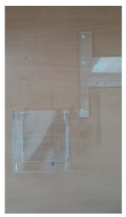
\includegraphics[scale=0.8]{bab2/kotak_sisi_belakang_kalibrasi.png}
		&
		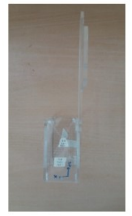
\includegraphics[scale=0.8]{bab2/kotak_sisi_samping_kalibrasi.png} \\
		\multicolumn{1}{c}{(a)} & \multicolumn{1}{c}{(b)} 
		
	\end{tabular}
	
	\begin{tabular}{ll}
		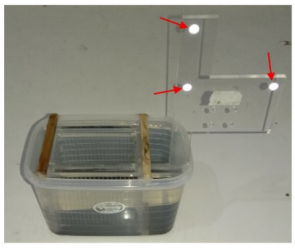
\includegraphics[scale=0.5]{bab2/kotak_kalibrasi_keseluruhan.png}\\
		\multicolumn{1}{c}{(c)}  
		
	\end{tabular}
	\caption{(a) Kotak sisi bagian belakang (b) Kotak sisi bagian samping, dan (c) Kotak kalibrasi yang diisi air}
	\label{fig:desain_kotak_kalibrasi}
\end{figure}


Kotak kalibrasi memiliki 19 lubang di sisi panjangnya, 11 di sisi lebar, serta 16 lubang pada sisi tinggi. Bagian kotak kalibrasi \textit{double-N} dilengkapi dengan benang nilon berukuran 0,45mm. Kotak bagian eksternal memiliki panjang sebesar 0,45mm, lebar 0,6mm, dan tinggi sebesar 0,7mm. Fungsi utma dari otak eksternal ini adalah untuk menampung cairan yang menjadi media untuk mentransmisikan sinyal dari \textit{probe ultrasound} ke benang. Adapun desain posisi kabel pada kotak kalibrasi dapat dilihat pada Gambar \ref{fig:desain_posisi_kabel}. 

\begin{figure}[htbp]
	\centering
	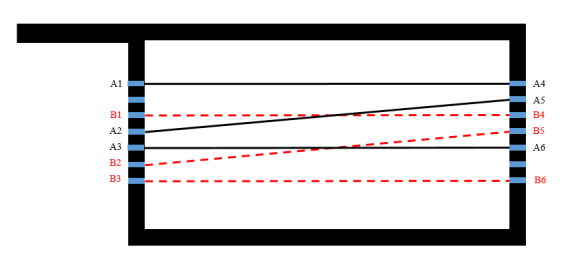
\includegraphics[scale= 0.7]{bab2/desain_posisi_kabel.png}
	\caption{Desain posisi benang pada kotak kalibrasi}
	\label{fig:desain_posisi_kabel}
\end{figure}



\subsection{Desain \textit{Marker} pada \textit{Probe}}
Marker pada \textit{probe ultrasound} memiliki 3 titik dalam sistem koordinat, yaitu M1, M2, dan M3. Titik M2 pada marker berfungsi sebagai pusat sistem koordinat pada \textit{probe ultrasound}. Sementara itu, marker pada kotak kalibrasi juga memiliki 3 titik sistem koordinat yaitu M4, M5, serta M6. Titik M6 pada marker kotak kalibrasi berfungsi sebagai pusat sistem koordinat pada kotak kalibrasi. Posisi marker dan sistem koordinat pada \textit{probe} dapat dilihat pada Gambar \ref{fig:posisi_kalibrasi}.

\begin{figure}[htbp]
	\centering
	\begin{tabular}{ll}
		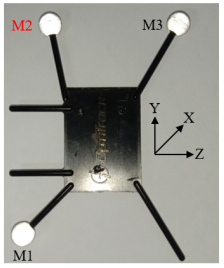
\includegraphics[scale=0.9]{bab2/marker_m2}
		&
		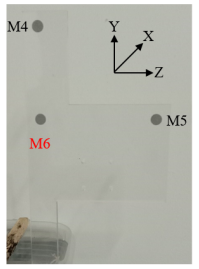
\includegraphics[scale=0.9]{bab2/marker_m6} \\
		\multicolumn{1}{c}{(a)} & \multicolumn{1}{c}{(b)}
	\end{tabular}
	\caption{(a) Posisi marker dan sistem koordinat Probe USG, M2 sebagai pusat koordinat probe. (b) Posisi marker dan sistem koordinat kotak kalibrasi, M6 sebagai pusat koordinat kotak kalibrasi.}
	\label{fig:posisi_kalibrasi}
\end{figure}




Adapun nilai dari M1, M2, dan M3 memiliki nilai yang dapat berubah - ubah. Dikarenaka adanya gerakan \textit{freehand} menggunakan \textit{probe ultrasound} saat proses kalibrasi. Namun marker M4, M5, dan M6 yang terletak pada kotak kalibrasi bersifat statis dikarenakan tidak mengikuti pergerakan \textit{freehand} \textit{probe} \textit{ultrasound}. Hasil pembacaan posisi marker, menghasilkan kumpulan titik dalam ruang tiga dimensi yang direpresentasikan dalam persamaan $M_i = x_j, y_j, z_j$. 


\subsection{Matriks Kalibrasi}
Proses ekstraksi matriks transformasi terdiri dari beberapa prosedur yang harus dilakukan. Pertama, menentukan vektor arah pada marker kotak kalibrasi. Kedua, menentukan vektor arah pada marker \textit{probe} \textit{ultrasound}. Prosedur yang terakhir yaitu menentukan matriks transformasi terhadap titik pusat marker kotak kalibrasi terhadap kamera \textit{optic track}. Titik pusat marker kotak kalibrasi direpresentasikan dengan variabel M2.

Arah vektor satuan pada sistem koordinat kotak kalibrasi didasarkan 3 sumbu yaitu $x,y,z$. Arah vektor satuan sumbu $x$ direpresentasikan dengan simbol \textbf{KX}, arah sumbu $y$ direpresentasikan dengan simbol \textbf{KY}, serta arah sumbu $z$ direpresentasikan dengan simbol \textbf{KZ}. Hal itu dapat dilihat pada Persamaan \ref{eq:persamaan_kz_1}.

\begin{equation}
	\textbf{KZ}\ =\ \frac{M5\ -\ M6}{\left|M5\ -\ M6\right|} \\
	=\ \frac{(x_5-x_6,y_5-y_6,z_5-z_6)}{\sqrt{{(x_5-x_6)}^2\ +\ {(y_5-y_6)}^2\ +\ {(z_5-z_6)}^2\ \ }}
	\label{eq:persamaan_kz_1}
\end{equation}

Dalam mengukur vektor satuan ke arah sumbu $x$ atau $KX$ dalam sistem koordinat kotak kalibrasi dibutuhkan Persamaan \ref{eq:persamaan_kx_1}. Kemudian variabel $KS$ merupakan vektor yang menggambarkan perpindahan dari titik $M4$ ke titik $M6$.

\begin{equation}
	\begin{aligned}
		\textbf{KX}\ =\ KS\ \times\ KZ \\[20pt]
		\textbf{KS}\ =\ M4\ -M6 =\ (x_4-x_6,y_4-y_6,z_4-z_6) \\[20pt] 
		\texbf{KX}\ =\ \frac{x_{KX}{,y}_{KX}{,z}_{KX}}{\sqrt{{(x_{KX})}^2+{(y_{KX})}^2+{(z_{KX})}^2}}
	\end{aligned}
	\label{eq:persamaan_kx_1}
\end{equation}

Adapun dalam mengukur vektor satuan ke arah sumbu $y$ ($KY$) dalam sistem koordinat kotak kalibrasi dibutuhkan Persamaan \ref{eq:persamaan_ky_1}. 

\begin{equation}
	\begin{aligned}
		\textbf{KY} = KZ \times KX \\[20pt]
		 \texbf{KY}\ =\ \frac{x_{KY}{,y}_{KY}{,z}_{KY}}{\sqrt{{(x_{KY})}^2+{(y_{KY})}^2+{(z_{KY})}^2}}
	\end{aligned}
	\label{eq:persamaan_ky_1}
\end{equation}  

Kemudian, hasil matrik transformasi yang diperoleh dengan titik pusat M6 terhadap sistem koordinat kamera \textit{optic track} (${_T^H}T$) dapat dilihat pada Persamaan \ref{eq:persamaan_matriks_m6}.

\begin{equation}
	{_T^H}T = \begin{bmatrix}x_{KX} & y_{KX} & z_{KX} & M6_x  \\x_{KY} & y_{KY} & z_{KZ} & M6_y \\x_{KZ} & y_{KZ} & z_{KZ} & M6_z \\0 & 0 & 0 & 1 \end{bmatrix}	
	\label{eq:persamaan_matriks_m6}
\end{equation}

Sementara itu, arah vektor satuan pada sistem koordinat \textit{probe ultrasound} didasarkan pada 3 sumbu yaitu $X$, $Y$, dan $Z$. Dalam mengukur vektor satuan ke arah sumbu $Z$ (\textbf{PZ}) dihitung berdasarkan Persamaan \ref{eq:persamaan_z_probe}.

\begin{equation}
	\textbf{PZ} = \frac{M3 - M2}{\left|M3 - M2 \right|} = \frac{(x_3-x_2, y_3 - y_2, z_3 - z_2)}{\sqrt{{(x_3 - x_2)^2 + (y_3 - y_2)^2 + (z_3 - z_2)^2 }}}
	\label{eq:persamaan_z_probe}
\end{equation} 

Dalam mengukur vektor satuan ke arah sumbu $X$ (\textbf{PX}) dihitung berdasarkan Persamaan \ref{eq:persamaan_px_probe}. Dimana \textbf{PS} merupakan vektor dari M1 terhadap M2 yang ditunjukkan pada Persamaan \ref{eq:persamaan_ps_probe}.

\begin{equation}
	\textbf{PS} = M1 - M2 = (x_1 - x_2, y_1 - y_2, z_1 - z_2)
	\label{eq:persamaan_ps_probe}
\end{equation}

\begin{equation}
	\begin{align}
		\textbf{PX} = \textbf{PS} \times \textbf{PZ}\\[10pt]
		\textbf{PX} = \frac{(x_{PX}, y_{PX}, z_{PX})}{\sqrt{{(x_{PX})^2 + (y_{PX})^2 + (z_{PX})^2}}}
	\end{align}
	\label{eq:persamaan_px_probe}
\end{equation}

Sementara itu, untuk mengukur vektor satuan ke arah sumbu $Y$ (\textbf{PY}) pada sistem koordinat \textit{probe ultrasound} dihitung berdasarkan Persamaan \ref{eq:persamaan_py_probe}. Dimana nilai vektor satuan \textbf{PY} diperoleh dari hasil perkalian antara vektor satuan ke arah sumbu $Z$ (\textbf{PZ}) dengan vektor satuan ke arah sumbu $X$ (\textbf{PX}).

\begin{equation}
	\begin{align}
		\textbf{PY} = \textbf{PZ} \times \textbf{PX} \\
		\textbf{PY} = \frac{(x_{PY}, y_{PY}, z_{PY})}{\sqrt{{(x_{PY}^2 + (y_{PY}^2 + (z_{PY}^2)}}}
	\end{align}	
	\label{eq:persamaan_py_probe}
\end{equation}

Dari perhitungan vektor satuan dari masing - masing arah sumbu $X$,$Y$,$Z$ pada sistem koordinat \textit{probe ultrasound}. Diperoleh matrik transformasi dari titik pusat M2 terhadap sistem koordinat \textit{probe ultrasound} (${_T^P}T$) dapat dilihat pada Persamaan \ref{eq:persamaan_matriks_m2}.


\begin{equation}
	{_T^P}T = \begin{bmatrix}x_{PX} & y_{PX} & z_{PX} & M2_x  \\x_{PY} & y_{PY} & z_{PZ} & M2_y \\x_{PZ} & y_{PZ} & z_{PZ} & M2_z \\0 & 0 & 0 & 1 \end{bmatrix}	
	\label{eq:persamaan_matriks_m2}
\end{equation}

Selanjutnya, citra \textit{ultrasound} (\textbf{U}) diubah melalui proses transformasi terhadap \textit{probe ultrasound} (\textbf{P}) menggunakan teknik transformasi homogen. Proses transformasi tersebut direpresentasikan dalam simbol $T{_U^P}$. Dengan menggunakan transformasi homogen, dapat diperoleh perubahan yang diperlukan pada citra \textit{ultrasound} untuk disesuaikan dengan posisi \textit{probe ultrasound}.



\subsection{Kalibrasi Skala Citra \textit{Ultrasound}}
Proses kalibrasi pada citra \textit{ultrasound} merupakan langkah penting untuk memastikan bahwa ukuran yang ditampilkan dalam citra tersebut sesuai dengan ukuran sebenarnya. Dalam hal ini, proses kalibrasi berfungsi untuk menentukan seberapa panjang setiap piksel dalam citra \textit{ultrasound} yang dihubungkan dengan ukuran nyata dalam satuan metrik.

Untuk melakukan kalibrasi ini diperlukan penggunaan perangkat lunak seperti \textit{Echo Wave II}. Perangkat lunak ini memungkinkan untuk mengambil pengukuran yang diperlukan dari citra yang dihasilkan. Kalibrasi ini dilakukan dengan mengukur skala citra baik secara horizontal maupun vertikal. Pengukuran secara horizontal ditandai dengan $S_x$ sedangkan pengukuran secara vertikal ditandai dengan $S_y$. Adapun pengukuran skala citra secara horizontal dan vertikal dapat dilihat pada Persamaan \ref{eq:persamaan_skala_citra}.

\begin{equation}
	\begin{aligned}
		S_x &= \frac{D_{px}}{D_{mx}} \\[10pt]
		S_y &= \frac{D_{py}}{D_{my}}
	\end{aligned}
	\label{eq:persamaan_skala_citra}
\end{equation}

Dimana variabel $D_{px}$ menunjukkan panjang piksel secara horizontal, $D_{mx}$ menunjukkan panjang metrik secara horizontal, $D_{py}$ menunjukkan panjang piksel secara vertikal, serta $D_{my}$ menunjukkan panjang metrik secara vertikal. Dalam proses pengukuran yang dilakukan menggunakan perangkat lunak \textit{Echo Wave II}, ditetapkan pengaturan kedalaman (\textit{depth}) sebesar 40. Ini memungkinkan untuk mendapatkan pengukuran yang akurat dalam satuan milimeter. Pengukuran ini dilakukan sejauh 20mm mengikuti garis lurus baik secara horizontal maupun vertikal. Setelah mendapatkan hasil pengukuran, langkah berikutnya yaitu membandingkannya dengan ukuran piksel pada citra yang dihasilkan oleh perangkat lunak. Hal ini dilakukan dengan mengukur jarak pikel dari ujung awal hingga ujung akhir secara horizontal dan vertikal. Adapun citra hasil pengukuran pada perangkat lunak \textit{Echo Wave II} dapat dilihat pada Gambar \ref{fig:result_echo_wave}.


\begin{figure}[htbp]
	\centering
	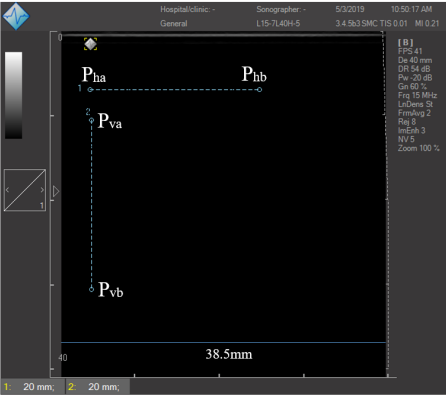
\includegraphics[scale= 0.6]{bab2/hasil_echo_wave.png}
	\caption{Citra hasil pengukuran menggunakan perangkat lunak \textit{Echo Wave II}}
	\label{fig:result_echo_wave}
\end{figure}

Dari hasil pengukuran yang telah dilakukan, ditemukan beberapa titik koordinat posisi. Posisi $P_ha(u_{xha}, v_{xha})$ = (133, 130), $P_hb(u_{xhb}, v_{xhb})$ = (383, 130), $P_va(u_{xva}, v_{xva})$ = (135,175) serta $P_vb = (135, 425)$. Dengan menggunakan data koordinat tersebut dan menerapkan persamaan \ref{eq:persamaan_jarak_koordinat} dapat menghitung panjang piksel. Adapun perhitungan panjang piksel menggunakan persamaan \ref{eq:persamaan_jarak_koordinat} diperoleh hasil panjang piksel secara horizontal $D_{px} =$ 250 piksel dan panjang piksel secara vertikal $D_{py} =$ 250 piksel.   


\begin{equation}
	\begin{aligned}
		D_{px} = \sqrt{(u_{xhb} - u_{xha})^2 + (v_{xhb} - v_{xha})^2 } \\[10pt]
		D_{py} = \sqrt{(u_{yhb} - u_{yha})^2 + (v_{yhb} - v_{yha})^2 }
	\end{aligned}
	\label{eq:persamaan_jarak_koordinat}
\end{equation} 

Dalam pengukuran ini diperoleh nilai panjang metrik secara horizontal $D_{mx}$ sebesar 20mm dan panjang metrik secara vertikal $D_{my}$ sebesar 20mm. Dari hasil tersebut, perbandingan skala secara horizontal $S_x$ = 20mm/250 piksel, sehingga didapatkan 1 piksel = 0,08mm. Perbandingan skala vertikal $S_y$ = 20mm/250 piksel sehingga 1 piksel =0,08mm.

%
%\section{Rekonstruksi 3D Citra \textit{Ultrasound}}
\section{Peningkatan Kualitas Citra}
Salah satu kelemahan dari citra \textit{ultrasound} sendiri adalah memiliki banyak \textit{noise}. Efek \textit{noise} yang berulang (\textit{multiplicative}) yang dilihat dalam bentuk granular (bintik) biasa disebut dengan \textit{speckle}\cite{made2020}. Tubuh menghasilkan \textit{speckle} dari kejadian terus-menerus dan sinyal pantul. Struktur dan karakteristik \textit{speckle} biasanya bergantung pada jaringan yang dicitrakan. Pengurangan \textit{speckle} sangat penting untuk meningkatkan kualitas dan pemahaman kita tentang pencitraan medis menggunakan \textit{ultrasound}. Adapun beberapa penelitian relevan terkait penghapusan \textit{noise} pada citra \textit{ultrasound}.

Penelitian yang dilakukan oleh Shodiq, dkk (2022)\cite{shodiq2022} membandingkan beberapa filter reduksi \textit{speckle} pada citra \textit{ultrasound} pembuluh darah serta memprediksi area pembuluh darah menggunakan model \textit{deep learning} U-Net. Adapun filter reduksi \textit{speckle} yang dibandingkan sebagai berikut (1) \textit{Wiener Filtering}; (2) \textit{Lee Filtering}; (3) \textit{Non-local means Filtering}; (4) \textit{Median Filtering}; (5) \textit{Total Variation Filter}; (6) \textit{Anisotropic Diffusion Filtering}; (7) \textit{Gaussian Filter}; serta (8) \textit{Wafelet Filter}. Adapun hasil penelitian yang diperoleh yaitu citra 2D \textit{ultrasound} gumpalan darah yang melalui proses reduksi \textit{speckle} dengan menggunakan filter \textit{Gaussian} mendapat hasil terbaik daripada beberapa filter reduksi \textit{speckle} yang lain dengan rata - rata akurasi sebesar 99\%, rata - rata nilai \textit{loss parameter} sebesar 0.0252, rata - rata nilai akurasi IoU sebesar 84.9\%,serta rata - rata nilai \textit{Hausdorff distance} sebesar 4.17. Prediksi \textit{mask area} menggunakan model \textit{deep learning} U-Net dengan filter \textit{gaussian} mendapat nilai 99.4\%.



\section{Segmentasi Citra \textit{Ultrasound}}
Segmentasi citra adalah teknik yang membagi citra digital menjadi subkelompok yang disebut segmen citra. Secara teknis, segmentasi adalah memberi label ke setiap piksel untuk menunjukkan objek, orang, atau elemen penting lainnya. Teknik ini biasanya digunakan untuk deteksi objek\cite{Yanhui2019}. Untuk menemukan objek yang diinginkan, algoritma segmentasi citra biasanya digunakan. Setelah objek ditemukan, detektor objek dapat beroperasi pada Region of Interest (RoI) yang telah ditentukan oleh algoritma tersebut. RoI itu sendiri mengurangi waktu inferensi dan meningkatkan akurasi. 

Output segmentasi citra merupakan kumpulan matriks atau mask dengan berbagai elemen yang menentukan kelas objek atau instance yang dimiliki setiap piksel\cite{kurmann2021mask}. Untuk segmentasi citra, mungkin bermanfaat untuk menggunakan beberapa heuristik yang relevan atau fitur gambar berkualitas tinggi. Algoritma segmentasi citra standar yang menggunakan teknik pengelompokan fitur tepi dan histogram bergantung pada fitur-fitur ini. Fitur warna merupakan salah satu contoh heuristik yang populer dalam proses segmentasi. Kontras program segmentasi citra juga bermanfaat karena dapat dengan mudah membedakan antara gelap dan terang.Teknik segmentasi citra tradisional yang bergantung pada heuristik semacam itu dapat dilakukan dengan cepat dan mudah, tetapi teknik tersebut sering kali memerlukan penyempurnaan untuk mendukung penggunaan heuristik yang dirancang secara manual dalam situasi tertentu\cite{jena2018survey}.

%\subsection{\textit{Machine Learning}}
%
%\subsection{\textit{Deep Learning}}
 
\subsection{Convolutional Neural Network (CNN)}
Salah satu jenis jaringan saraf tiruan yang digunakan untuk pengolahan data citra adalah Convolutional Neural Network (CNN). CNN menggunakan konsep konvolusi untuk mengekstrak karakteristik penting dari citra input, yang memungkinkan proses klasifikasi citra. CNN terdiri dari berbagai layer, termasuk layer convolution, layer pooling, dan layer fully-connected\cite{Mayank2020}. Layer pooling mengurangi overfitting sekaligus mengurangi dimensi feature map yang dibuat oleh layer convolution sebelumnya, dan layer convolution digunakan untuk mengekstrak fitur dari citra dengan menggunakan filter konvolusi yang diterapkan pada setiap sub-regional dari citra. Lapisan fully-connected mengklasifikasikan citra berdasarkan karakteristik yang diekstrak dari deretan layer sebelumnya.
CNN sudah banyak digunakan dalam bermacam aplikasi pengolahan citra semacam klasifikasi citra, deteksi objek, serta lain- lain. Beberapa penelitian relevan yang mengulas tentang CNN pada citra kedokteran antara lain sebagai berikut

Penelitian yang telah dilakukan oleh Sudha, dkk (2019)\cite{sudha2019} menunjukkan segmentasi area \textit{mask} citra arteri karotis menggunakan model CNN. Adapun hasil penelitian yang diperoleh yaitu model CNN lebih efektif digunakan untuk segmentasi daripada model SVM classifier dan model \textit{Radial Basis Function} dengan tingkat akurasi sebesar 99.33\%.


\subsection{U-Net - Deep Learning Model}
U-Net merupakan salah satu model \textit{deep learning} yang digunakan dalam segmentasi citra medis, khususnya pada citra 2D USG. Model U-Net dikembangkan oleh Olaf Ronneberger, dkk (2015) \cite{ronneberger2015u} dalam paper yang berjudul \textit{"U-Net: Convolutional Networks for Biomedical Image Segmentation"}.  Adapun keunggulan model U-Net sebagai model segmentasi sebagai berikut:
\begin{enumerate}
	\item U-Net telah terbukti memberikan hasil segmentasi yang baik dalam citra medis, dan karenanya sering digunakan dalam berbagai aplikasi segmentasi citra medis, termasuk citra ultrasound, MRI, dan CT-Scan.
	\item U-Net memiliki parameter yang lebih sedikit daripada model deep learning lainnya, sehingga pelatihannya menjadi lebih mudah dan waktu komputasinya lebih singkat.
	\item U-Net mengadaptasi arsitektur \textit{encoder} dan \textit{decoder}. Pada \textit{encoder} U-Net mengadaptasi arsitektur \textit{encoder} yang bertugas untuk mengekstraksi fitur - fitur tingkat tinggi dari citra. Sedangkan \textit{decoder} U-Net bertugas untuk mengembalikan informasi spasial ke dimensi asli citra untuk menghasilkan prediksi segmentasi.
	\item U-net juga memanfaatkan \textit{skip connection} yang menghubungkan bagian \textit{encoder} dan \textit{decoder}. Hal ini dapat membantu meningkatkan kemampuan segmentasi pada tingkat resolusi yang lebih rendah.
 \item U-Net dapat digunakan segmentasi \textit{multiclass} pada citra dua dmensi. Model ini dapat dilatih untuk mengidentifikasi dan memisahkan beberapa struktur atau objek yang berbeda dalam citra dua dimensi, seperti organ.
\end{enumerate}

% Penelitian yang dilakukan oleh Abdollahi, dkk (2020)\cite{abdollahi2020} bertujuan untuk segmentasi citra area jalan raya di Massachusets (negara bagian Amerika Serikat) dan Ottawa (Kanada). Yang menjadi tantangan dalam penelitian ini adalah citra yang akan disegmentasi memiliki resolusi yang tinggi serta segementasi area yang termasuk bagian dari jalan seperti bangunan, pohon, pejalan kaki, kendaraan, jalan pedesaan. Kelas - kelas tersebut memiliki karakteristik yang heterogen. Peneliti menggunakan model V-Net dengan menambahkan parameter \textit{Cross Entropy Dice Loss} (CEDL) yang digunakan untuk segmentasi area jalan. Hasil penelitian ini menyebutkan bahwa hasil akurasi segmentasi area jalan mendapatkan nilai 90.64\% untuk dataset Massachusetss serta 92.41\% untuk dataset Ottawa. Pada penelitian juga mengkomparisikan hasil akurasi menggunakan U-Net + CEDL dengan model FCN, Segnet, dan U-Net dimana masing - masing mendapatkan akurasi sebesar 1.09\%, 2.45\%, dan 0.39\% untuk dataset Massachusets. Kemudian nilai 7.21\%, 1.86\%, dan 2.68\% untuk dataset Ottawa.
Penelitian yang telah dilakukan oleh Yang, dkk (2022)\cite{yang2022ax}
melakukan segmentasi pankreas. Dalam penelitian ini, peneliti mengusulkan model segmentasi yaitu AX-Unet yang merupakan U-Net termodifikasi dengan memadatkan piramida untuk mempelajari informasi lokai dan mengekstrak informasi kontekstual multi-level untuk mengurangi kehilangan informasi selama pengurangan sampel. Peneliti juga memperkenalkan konvolusi baru pada peta fitur di setiap level untuk mencapai pemisahan informasi antar saluran. Kemudian peneliti juga mengusulkan fungsi batas eksplisit guna mengatasi batas buram. Data yang digunakan dalam penelitian ini adalah dataset \textit{Pancreas}-CT publik, dataset NIH-Pancreas-CT, serta datataset pankreas medis \textit{decathlon}. Hasil eksperimen menunjukkan bahwa model yang diusulkan oleh peneliti dapat mengungguli metode terbaru dalam segmentasi citra CT Pankreas. Dengan membandingkan output fitur yang diekstraksi dari model yang diusulkan, peneliti menemukan bahwa daerah pankreas pada orang normal dan pasien penderita tumor pankreas menunjukkan perbedaan yang signifikan.

Penelitian yang dilakukan oleh Behboodi, dkk (2019)\cite{behboodi2019ultrasound} mengusulkan penggunaan citra \textit{ultrasound} sebagai dataset untuk \textit{training} pada model \textit{deep learning} U-Net yang diujikan pada data yang diakuisisi melalui phantom. Kontribusi penelitian ini, peneliti melatih menggunakan data \textit{envelope} dan citra B-Mode.

% Penelitian yang dilakukan oleh Dangoury, dkk\cite{Dangoury2022} menguji implementasi model V-Net dalam segmentasi citra dua dimensi \textit{ultrasound}. Tidak hanya itu, hasil dari penelitian tersebut dibandingkan dengan model U-Net dan model U-Net++ berdasarkan empat \textit{Loss Function} seperti \textit{ Cross-Entropy (CE)}, \textit{Dice Similarity Coefficient} (DSC), Focal loss (FL) and \textit{Focal Tversky Loss}. 

Model U-Net memiliki tiga lapisan utama yaitu \textit{encoder}, \textit{skip connection}, dan \textit{decoder}. Pada bagian \textit{encoder} berfungsi untuk mengimplementasikan fitur setiap layer pada citra input. Kemudian bagian \textit{decoder} berfungsi untuk mengubah fitur yang menjadi output pada bagian \textit{encoder} menjadi citra prediksi \textit{mask}. Bagian \textit{skip connection} berfungsi untuk menghubungkan bagian \textit{encoder} dengan \textit{decoder} pada model U-Net. Adapun langkah - langkah model U-Net sebagai berikut:
\begin{enumerate}
    \item Citra dimasukkan ke dalam layer pada bagian \textit{encoder}.
    \item Citra akan diekstraksi fiturnya oleh setiap layer yang ada pada bagian \textit{encoder}.
    \item Output dari bagian \textit{encoder} berupa fitur dikirimkan ke bagian \textit{decoder} melalui \textit{skip connection}.
    \item Layer - layer yang ada pada bagian \textit{decoder} menggabungkan fitur menjadi citra prediksi \textit{mask}.
    \item Hasil prediksi \textit{mask} menjadi output dari segmentasi menggunakan model U-Net.
\end{enumerate}

\begin{figure}[htbp]
	\centering
	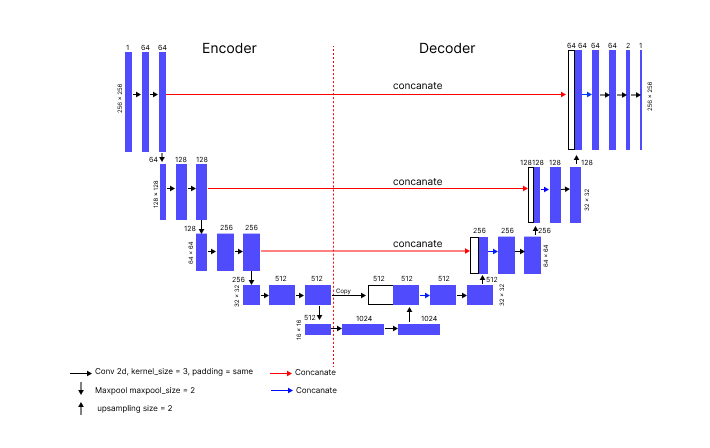
\includegraphics[scale= 0.6]{bab2/mondelUnetBab2.png}
	\caption{Arsitektur U-Net}
	\label{fig:modelU-Net}
\end{figure}

%\subsection{Konfigurasi \textit{Hyperparameter}}
%\subsubsection{\textit{Epoch}}
%\subsubsection{\textit{Batch}}
%\subsubsection{\textit{Iterasi}}
%\subsubsection{\textit{Optimizer}}
%\subsubsection{\textit{Loss Function}}
%\subsubsection{\textit{Activation Function}}



\subsection{Metric Evaluation}
\subsubsection{Akurasi}
Akurasi merupakan metrik evaluasi yang mengukur efisiensi suatu model pembelajaran mesin dalam menghasilkan prediksi yang valid. Adapun akurasi dapat dilihat pada persamaan berikut. 

\begin{equation}
	\text{Akurasi} = \frac{TP + TN}{TP + TN + FP + FN}
\end{equation}

\subsubsection{Intersection Over Union (IOU)}
\textit{Intersection over Union} (IoU) digunakan untuk mengukur kemiripan antara dua objek 2D dalam sebuah citra\cite{rezatofighi2019generalized}. Nilai IoU diperoleh melalui perhitungan area irisan antara area objek yang sebenarnya (\textit{ground-truth}) ($X$) dengan area yang dihasilkan oleh model segmentasi (\textit{masking predicted}) ($Y$). Kemudian hasil perhitungan area irisan antara dua objek tersebut dibagi dengan hasil perhitungan area gabungan dari 2 objek tersebut. Adapun persamaan IoU dapat dilihat pada Persamaan \ref{eq:persamaan1}. 

\begin{equation}
	\label{eq:persamaan1}
	\textit{IoU} = \frac{\textit{Area Irisan (Intersection)}}{\textit{Area Gabungan (Union)}} = \frac{|\ X \cap Y\ |}{|\ X \cup Y\ |}
\end{equation}


Hasil pengukuran IoU terdiri dari rentang nilai mulai dari 0 hingga 1. Apabila nilai IoU mendekati nilai 0, maka hasil prediksi segmentasi tidak mirip dengan bentuk \textit{ground truth}. Sebaliknya, apabila perhitungan IoU mendekati nilai 1, maka hasil prediksi segmentasi mirip dengan \textit{groundtruth}.

\begin{figure}[htbp]
	\centering
	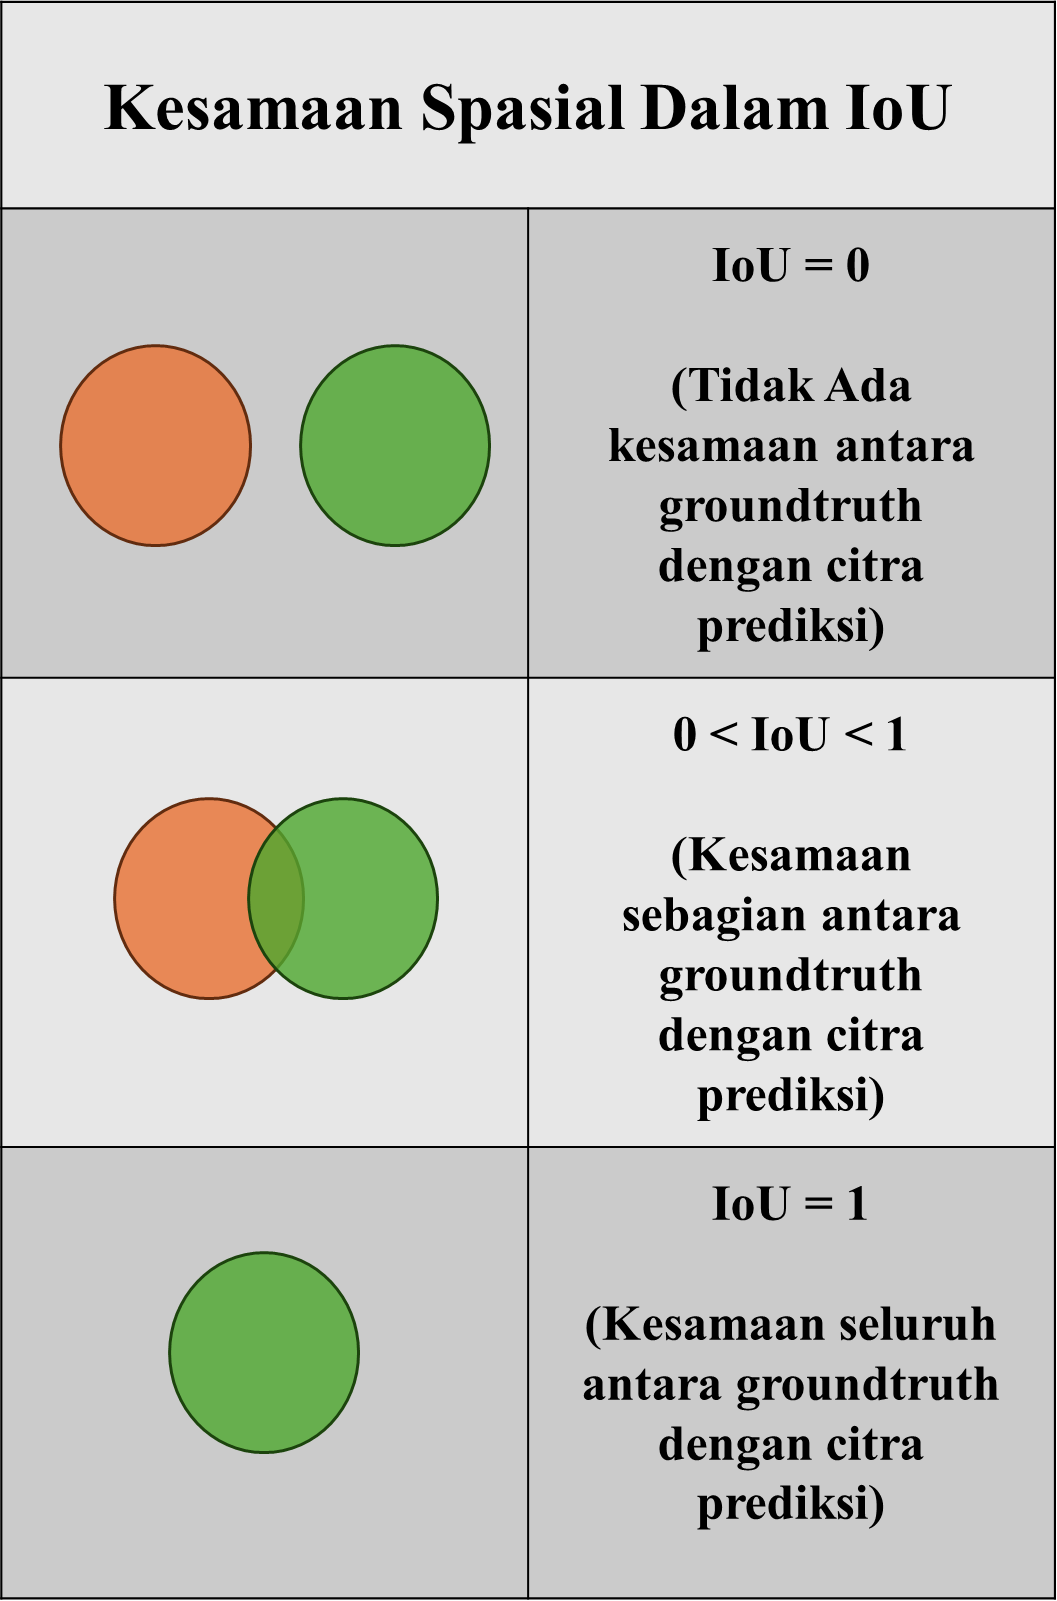
\includegraphics[scale= 0.2]{bab2/iou_spasial.png}
	\caption{Representasi Kesamaan dalam nilai IoU}
	\label{fig:iou_spasial}
\end{figure}

\subsubsection{\textit{Dice Coefficient}}
\textit{Dice coefficient} merupakan metrik evaluasi digunakan untuk mengukur tingkat kesesuaian antara 2 citra yaitu citra area objek sebenarnya(\textit{ground-truth}) dengan citra prediksi dari hasil segmentasi. Nilai \textit{dice coefficient} diperoleh dari 2 kali ukuran area irisan antara area objek yang sebenarnya (\textit{ground-truth}) ($X$) dengan area yang dihasilkan oleh model segmentasi (\textit{masking predicted}) ($Y$). Kemudian hasil perhitungan dua kali area irisan antara dua objek tersebut dibagi dengan hasil perhitungan area gabungan dari 2 objek tersebut. Adapun perhitungan \textit{dice coefficient} dapat dirumuskan sebagai berikut. 

\begin{equation}
	\textit{Dice(X,Y)} = \frac{2 \times \textit{Area Irisan (Intersection)}}{\textit{Area Gabungan (Union)}} = \frac{|\ X \cap Y\ |}{|\ X \cup Y\ |}
\end{equation}

Hasil pengukuran \textit{dice coefficient} terdiri dari rentang nilai mulai dari 0 hingga 1. Apabila nilai \textit{dice coefficient} mendekati nilai 0, maka hasil prediksi segmentasi tidak mirip dengan bentuk \textit{ground truth}. Sebaliknya, apabila perhitungan \textit{dice score} mendekati nilai 1, maka hasil prediksi segmentasi mirip dengan \textit{groundtruth}.

\begin{figure}[htbp]
	\centering
	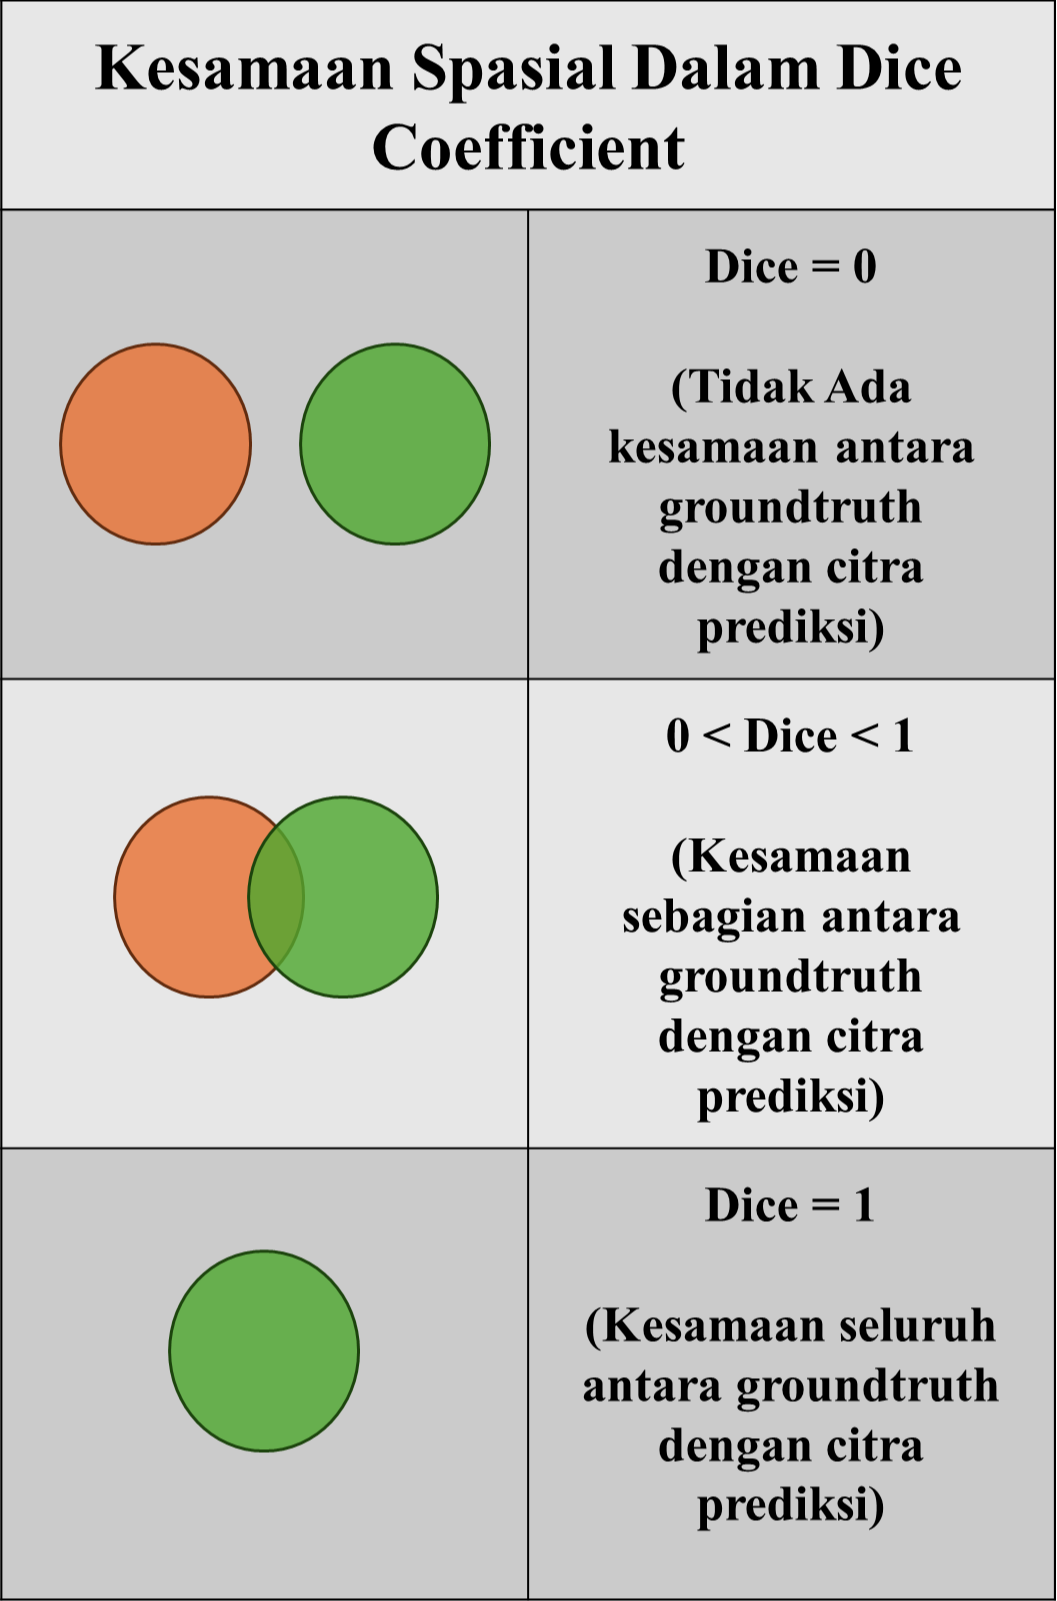
\includegraphics[scale= 0.2]{bab2/dice_spasial.png}
	\caption{Representasi Kesamaan dalam nilai \textit{dice coeffficient}}
	\label{fig:dice_spasial}
\end{figure}


\subsubsection{\textit{Hausdorff Distance}}
\textit{Hausdorff distance} merupakan metode pengukuran yang digunakan untuk menilai seberapa baik performa sebuah segmentasi citra, khususnya citra medis. Citra medis yang digunakan dalam peneltian ini adalah citra \textit{ultrasound}. Adapun cara kerja dari perhitungan \textit{hausdorff distance} yaitu menghitung jarak antara dua himpunan titik yang berasal dari 2 citra yaitu citra dengan area objek sebenarnya (\textit{groundtruth}) ($A$) dan citra dengan  area yang dihasilkan oleh model segmentasi (\textit{masking predicted})($B$). Adapun perhitungan \textit{hausdorff distance} dapat dirumuskan sebagai berikut. 

\begin{equation}
	hd(A,B)=max_{i,j}\left\{d(A_i,B), d(B_j, A)\right\}
	\label{eq13}
\end{equation}

Dimana,

\begin{equation}
	d(A_i,B)=min_{k}\left\{d(A_i,B_k)\right\}
\end{equation}

\begin{equation}
	d(B_j,A)=min_{k}\left\{d(B_j,A_k)\right\}
\end{equation} 

Berdasarkan definisi diatas, untuk menghitung jarak $d(A_i, B)$ menggunakan \textit{euclidean distance}. Variabel $hd(A, B)$ merupakan jarak terjauh yang ditempuh dari piksel $A$ ke bagian tepi dari $B$. Nilai \textit{hausdorff distance} yang rendah, yaitu mendekati 0, menunjukkan bahwa ada kemiripan yang tinggi antara objek - objek pada kedua citra tersebut. Hal ini dapat diartikan sebagai area prediksi dari hasil segmentasi sangat mirip dengan area sebenarnya (\textit{groundtruth}). Namun, apabila nilai \textit{haudorff distance} tidak mendekati 0, maka ada perbedaan yang signifikan antara dua titik. Sehingga terindikasi bahwa hasil segmentasi kurang akurat.



% \section{Cara Penulisan Persamaan}
% Cara menulis persamaan  inline pada text $\sum_{i=1}^{N} x_iy_i$


% Contoh Integral
% \begin{equation}\label{eq:persamaan1}
% y=\int_{0}^{2\pi} cos(x) dx
% \end{equation}
% Persamaan \ref{eq:persamaan1} adalah contoh menulis fungsi $cos(\alpha x)$ dari $0\le x\le 2\pi$.\\
% Menjajarkan persamaan
% \begin{align}
% y&=\int_{0}^{2\pi}cos(x)dx\\
% &=sin(x)|_0^{2\pi}\\
% &=sin(2\pi)-sin(0)\\
% &=0
% \end{align}
% Persamaan \ref{eq:matrix} adalah matrix.
% \begin{equation}\label{eq:matrix}
% \textbf{X}=\begin{bmatrix}
% x_{11}&x_{12}&\cdots&x_{1m}\\
% x_{21}&x_{22}&\cdots&x_{2m}\\
% \vdots&\vdots&\ddots&\vdots\\
% x_{n1}&x_{n2}&\cdots&x_{nm}
% \end{bmatrix}
% \end{equation}
% \vspace{1ex}
% \section{Cara Penulisan Tabel}
% \begin{table}[H]
% 	\caption{Tabel Contoh}
% 	\begin{tabular}{|l|l|l|l|}
% 		\hline
% 		No & X & Y & C \\ \hline
% 		1 & 0 & 0 & 1 \\ \hline
% 		2 & 0 & 1 & 0 \\ \hline
% 		3 & 1 & 0 & 0 \\ \hline
% 		4 & 1 & 1 & 0 \\ \hline
% 	\end{tabular}
% \end{table}


% \begin{table}[H]
% 	\label{tab:tabelcontoh2}
% 	\caption{Tabel ini contoh 2}
% 	\begin{tabular}{|l|l|l|l|}
% 		\hline
% 		\multirow{2}{*}{\textbf{No}} & \multicolumn{3}{l|}{\textbf{Data}} \\ \cline{2-4} 
% 		& \textbf{x} & \textbf{y} & \textbf{z} \\ \hline
% 		\textbf{1} & \textbf{0.1} & \textbf{0.2} & \textbf{0.3} \\ \hline
% 		\textbf{2} & \textbf{0.4} & \textbf{0.5} & \textbf{0.6} \\ \hline
% 	\end{tabular}
% \end{table}
% Pada Tabel \ref{tab:tabelcontoh2} di tunjukan cara membuat tabel.


% \begin{sidewaystable}
% 	\centering
% 	\caption{Tabel ke samping}
% 	\begin{tabular}{|l|l|l|l|}
% 		\hline
% 		\multirow{2}{*}{\textbf{No}} & \multicolumn{3}{l|}{\textbf{Data}} \\ \cline{2-4} 
% 		& \textbf{x} & \textbf{y} & \textbf{z} \\ \hline
% 		\textbf{1} & \textbf{0.1} & \textbf{0.2} & \textbf{0.3} \\ \hline
% 		\textbf{2} & \textbf{0.4} & \textbf{0.5} & \textbf{0.6} \\ \hline
% 	\end{tabular}
	
% \end{sidewaystable}
% \newpage
% \section{Cara Meletakan Gambar}
% \begin{figure}[H]
% 	\centering
% 	
\includegraphics[width=0.5\linewidth]{bab2/LambangTeknikElektro}
% 	\caption{Lambang Teknik dengan Ukuran 0.5 Lebar Kertas}
% 	\label{fig:lambangteknikelektro}
% \end{figure}
% \begin{figure}[H]
% 	\centering
% 	
\includegraphics[width=0.2\linewidth]{bab2/LambangTeknikElektro}
% 	\caption{Lambang Teknik dengan Ukuran 0.2 lebar kertas}
% 	\label{fig:lambangteknikelektro2}
% \end{figure}
% \begin{figure}[H]
% 	\centering
% 	
\includegraphics[width=0.5\linewidth]{bab2/LambangTeknikKOmputer}
% 	\caption{Lambang Teknik Komputer  }
% 	\label{fig:lambangteknikkomputer}
% \end{figure}
% \section{Cara Membuat  sitasi}

% Ini adalah cara  sitasi ke buku menggunakan cite\{Refferensi\}\\

% Contoh : sitasi ke 1
%  \cite{Brathwaite2009}.\\
% Daftar referensi terletak pada file 
% \textit{lainnya/pustaka.bib}\\

% contoh  sitasi ke 2
% \cite{Friedman1997}
% \newline
% \section{Algoritma}
% Contoh Algoritma

% \begin{algorithm}[H]
% 	\SetKwInOut{Input}{Input}
% 	\SetKwInOut{Output}{Output}
	
% 	\underline{function Euclid} $(a,b)$\;
% 	\Input{Two nonnegative integers $a$ and $b$}
% 	\Output{$\gcd(a,b)$}
% 	\eIf{$b=0$}
% 	{
% 		return $a$\;
% 	}
% 	{
% 		return Euclid$(b,a\mod b)$\;
% 	}
% 	\caption{Euclid's algorithm for finding the greatest common divisor of two nonnegative integers}
% \end{algorithm}
% \newpage
% \section{Tools Online Yang Cukup Membantu}
% Beberapa tools yang dapat digunakan untuk menulis tesis dengan latex.
% \subsection{Online equation editor: HostMath }
% \begin{center}
% 	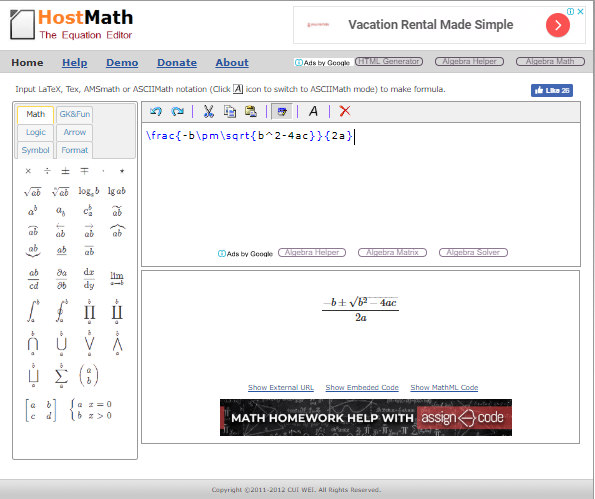
\includegraphics[width=1\linewidth]{bab2/Hosmath}
% 	\captionof{figure}{http://hostmath.com/}
% 	\label{fig:hosmath}
% \end{center}




% \newpage
% \subsection{Detexify LaTeX handwritten symbol recognition}
% \begin{center}
% 	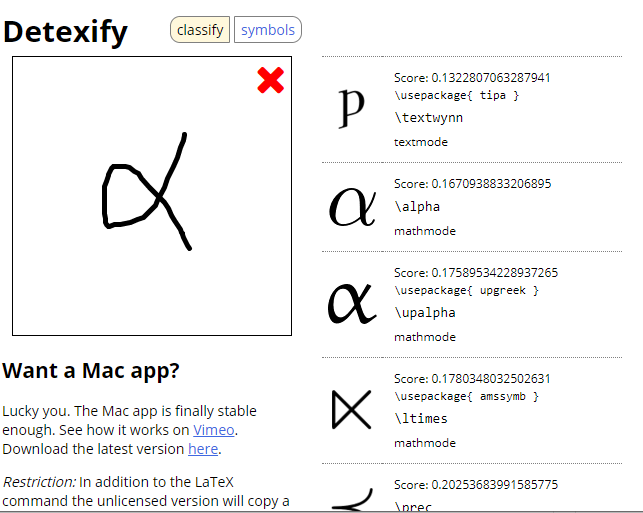
\includegraphics[width=\linewidth]{bab2/Detexify}
% 	\captionof{figure}{http://detexify.kirelabs.org/classify.html}
% 	\label{fig:detexify}
% \end{center}
% \newpage
% \subsection{Tables Generator }
% \begin{center}
	
% 	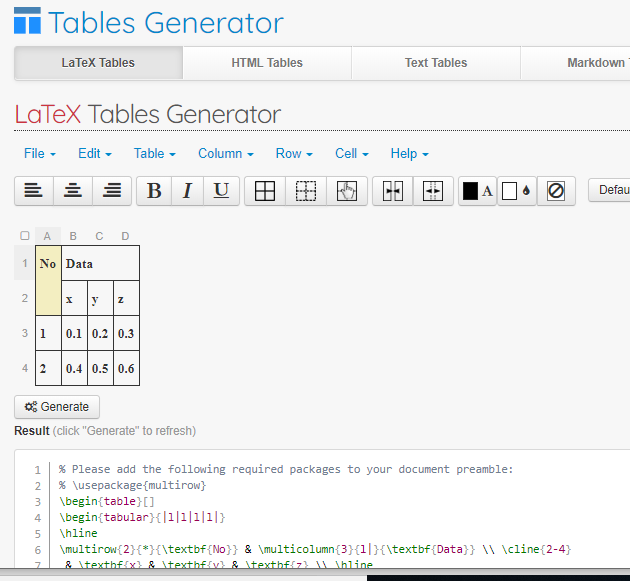
\includegraphics[width=0.7\linewidth]{bab2/TabelGenerator}
% 	\captionof{figure}{https://www.tablesgenerator.com/}
% 	\label{fig:tabelgenerator}
% \end{center}

% \subsection{Long Table}
% \begin{landscape}

% \begin{spacing}{1}	
% \begin{longtable}{|p{3cm}| p{7cm} | p{7cm} | p{7cm}|}\label{table:Posisidankontribusipenelitian}\\
% 	\caption{Posisi dan kontribusi penelitian}\\
% 	%\toprule
% 	\hline
% 	\nohyphens{\textbf{Topik riset Registrasi}}  & \textbf{Metode}  &\nohyphens{\textbf{Kontribusi Peneliti Lain}}&\nohyphens{\textbf{Kontribusi Peneliti}} \\ 
% 	%\midrule
% 	\hline
% 	\endfirsthead
% 	\caption{Posisi dan kontribusi penelitian \textit{(Lanjutan..)}}\\
% 	%\toprule
% 	\hline
	
% 	\nohyphens{\textbf{Topik riset Registrasi}}  & \textbf{Metode}  &\nohyphens{\textbf{Kontribusi Peneliti Lain}}&\nohyphens{\textbf{Kontribusi Peneliti}} \\ 
% 	%\midrule
% 	\hline
% 	\endhead
% 	\multicolumn{4}{r}{{(\textit{Tabel bersambung..})}} \\
% 	\endfoot
% 	\endlastfoot 
% 	Ekstraksi feature& 	Kurvature  pada suatu titik di hitung pada beberapa skala dengan fitting  permukaan ke  titik lokal pada berbagai macam ukuran. (Ho dan Gibbins, 2009) & 	Multi-scale  Feature Extraction from 3D Meshes and Unstructured Point Cloud& \\ \hline 
% 	Estimasi vektor normal& 	Fitting tangen vektor pada  data titik untuk menentukan vektor normal berbasis local voronoy mesh. (OuYang dan Feng, 2005) & 	Metoda baru untuk estimasi vektor normal. & \\ \hline 
% 	Estimasi principal direction& 	The Adjacent-Normal Cubic Approximation 
% 	(Goldfeather dan Interrante, 2004) & 	Estimasi principal direction dan vektor normal pada permukaan dengan noise yang tinggi.&\\ \hline 
% 	Registrasi berbasis fitur permukaan. & 	Normal distribution transform.
% 	(Pathak, Birk,Vaskevicius dan Poppinga, 2010) & 	Online registrasi pose untuk menentukan posisi robot. & 	 \\ \hline 
% 	Registrasi 3D berbasis warna. & 	Warna rgb (Johnson dan Kang, 1997). 
% 	(Douadi dkk., 2006) & 	Menggantikan fitur geometri ketika informasi geometri permukaan tidak mencukupi. & 	\\ \hline 
% 	& 	Registrasi berbasis warnoHSV. (Druon, Aldon dan Crosinier, 2006) & 	Registrasi tidak di pengaruhi oleh intensitas warna. & 	\\ \hline 
% 	& 	Registrasi dengan Modified color ICP kombinasi antara warna RGB dengan jarak ecludiean.  (Joun,Ang,Kang,Chung dan Yu(2009) & 	Registrasi untuk lingkungan 3D. & 	\\ \hline 
% 	Registrasi Berbasis geometri permukaan.& 	Registrasi dengan angular invariant feature.  (Jiang dkk., 2009) & 	\textit{Angular  invariant feature} invariant terhadap rotasi dan skala. & 	\\ \hline 
% 	& 	Point  Feature Histograms (PFH)  robust multi-dimensional features. (Rusu, Blodow, Marton, Soos dan Beetz, 2007) & 	Kombinasi curvature, vektor normal dan vektor pcincipal direction. & 	\\ \hline 
% 	& 	Fitting quadratik surface  (Chen dan Bhanu, 2007) & 	Permukaan lokal sebagai deskriptor untuk Kombinasi curvature, vektor normal dan vektor pcincipal direction. & 	\\ \hline 
% 	& 	& 	& 	Registrasi Citra  2D multiview untuk penangkap gerak manusia
% 	Semina Sesindo 2010 (Yuniarno, Mardi, Sumpeno dan Hariadi, 2010)\\ \hline 
% 	& 	& 	& 	Registrasi permukaan berbeasis surface curvature feature.
% 	Jurnal Jatit  (Yuniarno, Hariadi dan Purnomo, 2013a) \\ \hline 
% 	Outlier Removal& 	Tiga konstrain untuk memperoleh korspondensi akurat. 
% 	(Liu, 2008)& 	Korespondensi yang akurat& 	\\ \hline 
% 	& 	Dua  konstrain untuk memperoleh korspondensi akurat. 
% 	(Xin dan Pu, 2010)& 	Perbaikan tiga konstrain yang diusulkan oleh Liu dengan meletakan origin ke titik berat permukaan.& 	\\ \hline 
% 	& 	& 	& 	perbaikan korespondensi 
% 	dengan rigid constraint berbasis dua titik referensi dan surface curvature feature Jurnal Kursor (Yuniarno, Hariadi dan Purnomo, 2013b)\cite{Brathwaite2009} \\ \hline 
% \end{longtable}

% \end{spacing}

% \end{landscape}
% \section{Tabel Rencana Penelitian }


% \begin{table}[h!]
% 	\caption{Rencana Penelitian}
% 	\begin{tabular}{|l|l|l|l|l|l|l|l|l|l|}
% 		\hline
% 		& \multicolumn{9}{c|}{\textbf{Semester Ke}} \\ \cline{2-10} 
% 		\multirow{-2}{*}{} & 1 & 2 & 3 & 4 & 5 & 6 & 7 & 8 & 9 \\ \hline
% 		Rencana 1 & \cellcolor[HTML]{000000} & \cellcolor[HTML]{000000} & \cellcolor[HTML]{000000} & \cellcolor[HTML]{000000} & \cellcolor[HTML]{000000} &  &  &  &  \\ \hline
% 		Rencana 2 &  &  & \cellcolor[HTML]{000000} & \cellcolor[HTML]{000000} & \cellcolor[HTML]{000000} & \cellcolor[HTML]{000000} & \cellcolor[HTML]{000000} &  &  \\ \hline
% 		Rencana 3 &  &  &  &  &  & \cellcolor[HTML]{000000} & \cellcolor[HTML]{000000} & \cellcolor[HTML]{000000} & \cellcolor[HTML]{000000} \\ \hline
% 		Rencana 4 &  & \cellcolor[HTML]{000000} & \cellcolor[HTML]{000000}{\color[HTML]{000000} } & \cellcolor[HTML]{000000}{\color[HTML]{000000} } & \cellcolor[HTML]{000000}{\color[HTML]{000000} } & \cellcolor[HTML]{000000}{\color[HTML]{000000} } & \cellcolor[HTML]{000000}{\color[HTML]{000000} } & \cellcolor[HTML]{000000}{\color[HTML]{000000} } & \cellcolor[HTML]{000000}{\color[HTML]{000000} } \\ \hline
% 	\end{tabular}
% \end{table}




	\cleardoublepage
	

\chapter{METODOLOGI}
\label{sec:chap3_metodologi}



\section*{ }
Pada penelitian yang berjudul "Segmentasi Gumpalan Darah Vena Pada Citra \textit{Ultrasound} Menggunakan U-Net" nantinya akan terdiri dari empat langkah utama yaitu (1) data 2D citra \textit{ultrasound} gumpalan darah; (2) \textit{preprocessing}; (3) segmentasi gumpalan darah; serta (4) visualisasi 3D gumpala darah. Adapun empat langkah utama tersebut dapat dilihat pada Gambar \ref{fig:blokdiagram}.
\begin{figure}[H]
	\centering
	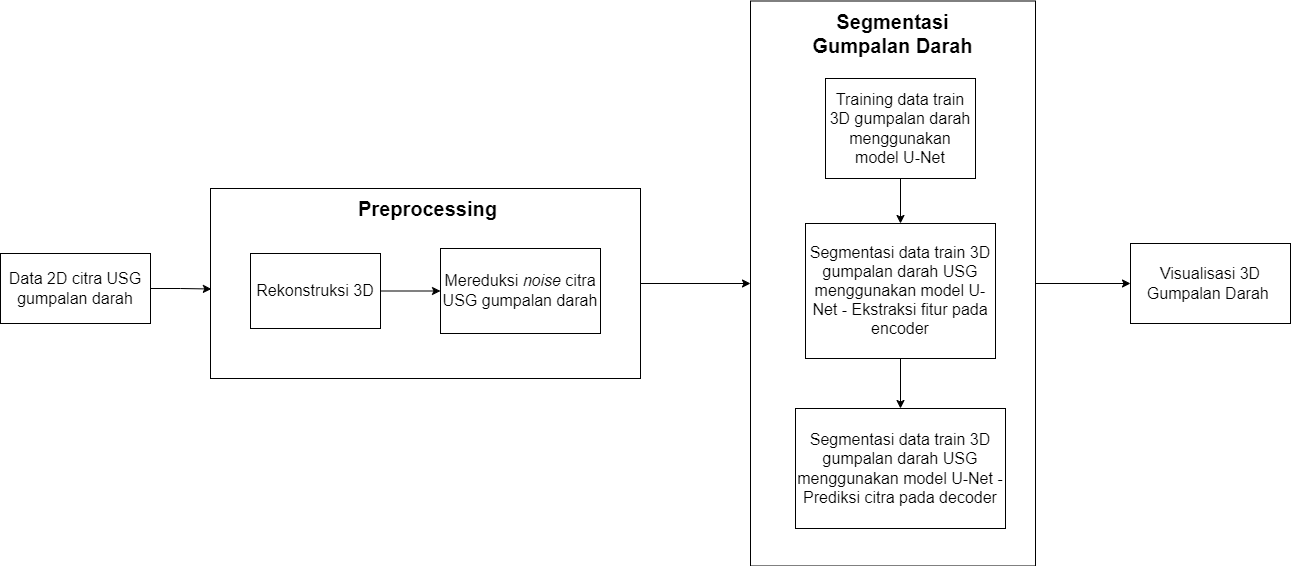
\includegraphics[width=\linewidth]{bab3/diagram-block version 2.png}
	\caption{Blok Diagram Segmentasi Gumpalan Darah Vena Pada Citra Ultrasound Menggunakan U-Net}
	\label{fig:blokdiagram}
\end{figure}


\section{Data 2D Citra \textit{Ultrasound} Gumpalan Darah Vena}

Data 2D citra ultrasound gumpalan darah (\textit{thrombus}) pada pembuluh darah vena diperoleh dari lima pasien dari penderita \textit{Deep Vein Thrombosis} (DVT) serta hasil akuisisi citra 2D ultrasound menggunakan peralatan seperti \textit{phantom}, USG \textit{Telemed-SmartUs}, \textit{Probe}, serta \textit{Optitrack}. Aturan dan syarat tertentu harus diikuti dalam penelitian ini sebelum memulai proses akuisisi citra ultrasound, untuk memastikan bahwa prosedur tersebut berjalan dengan baik. 

\subsection{Perangkat Akuisisi Citra \textit{Ultrasound} Gumpalan Darah Vena}
Penelitian ini menggunakan data citra ultrasound dua dimensi (2D) gumpalan darah (\textit{thrombus}) yang ada pada pembuluh darah vena. Data ini diakuisisi dari phantom yang terbuat dari balon panjang. Phantom balon panjang dirancang khusus oleh peneliti agar menyerupai bentuk pembuluh darah vena manusia, dan di dalamnya dimasukkan lemak sapi. Penggunaan lemak sapi dipilih karena struktur lemak sapi menyerupai bentuk \textit{thrombus} yang biasa ditemui di dalam pembuluh darah pasien penderita DVT. 

Penggunaan \textit{phantom} balon panjang ini bertujuan untuk menciptakan kondisi yang mirip dengan kondisi penderita DVT dimana \textit{thrombus} terbentuk di dalam pembuluh darah vena. Serta peneliti juga mengamati dan menganalisis bentuk \textit{thrombus} melalui citra ultrasound. Oleh karena itu penggunaan \textit{phantom} balon panjang sangat penting karena menjadi sumber utama  simulasi \textit{thrombus} yang terdapat pada pembuluh darah vena. Adapun \textit{phantom} balon panjang yang digunakan dalam penelitian ini serta hasil pencitraan \textit{ultrasound} menggunakan \textit{phantom} balon panjang dapat dilihat pada Gambar \ref{Fig:phantom_baloon}

\begin{figure}[h]
        \centering
	\begin{tabular}{ll}
		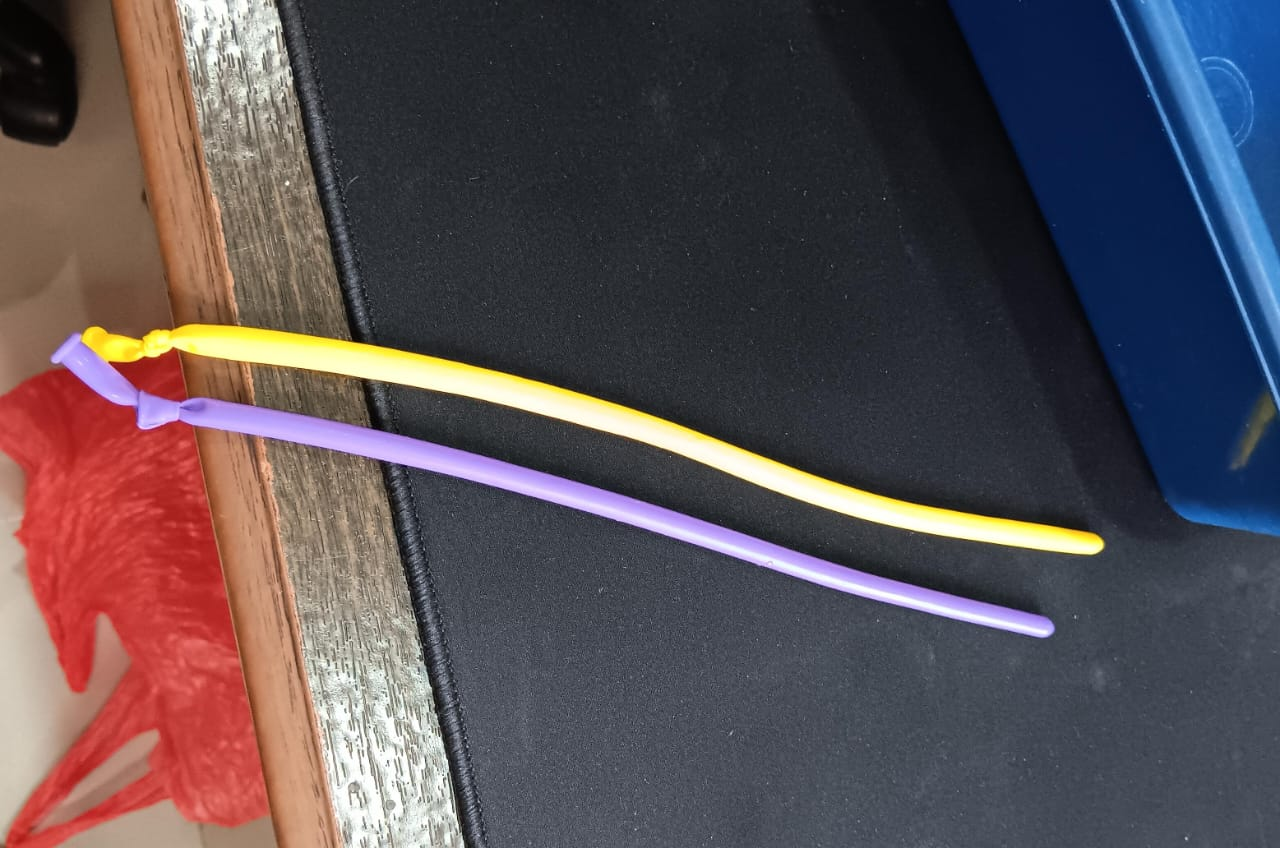
\includegraphics[scale=0.18]{bab3/phantom_balon.jpg}
		&
		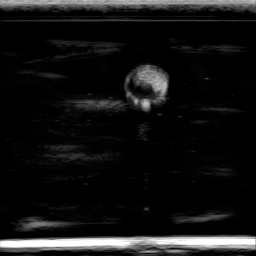
\includegraphics[scale=0.6]{bab3/img_thrombus.png} \\
		\multicolumn{1}{c}{(a)} & \multicolumn{1}{c}{(b)}
	\end{tabular}
	\caption{(a) \textit{Phantom} Balon Panjang (b) Hasil Pencitraan \textit{Ultrasound} Menggunakan \textit{Phantom} Balon Panjang.}
	\label{Fig:phantom_baloon}
\end{figure}

Selain menggunakan \textit{phantom} balon panjang, dalam beberapa percobaan peneliti menggunakan data \textit{thrombus} pada pembuluh darah vena yang diperoleh dari lima pasien penderita DVT dengan total 317 citra. \textit{Thrombus} penderita DVT terbentuk di dalam pembuluh darah vena bagian kaki. Data \textit{thrombus} ini menyajikan informasi visual yang dihasilkan dari pemindaian menggunakan sensor ultrasonografi (USG) yang memperlihatkan lokasi dan karakteristik \textit{thrombus} dalam pembuluh darah vena pada ke lima pasien tersebut.Penggunaan data penderita DVT ini bertujuan untuk meningkatkan variasi dalam dataset yang diterapkan selama pelatihan model \textit{deep learning} U-Net, sehingga model tersebut bisa melakukan segmentasi area gumpalan darah pada area pembuluh darah vena dengan tingkat keakuratan yang lebih tinggi. Adapun citra ultrasound \textit{thrombus} penderita DVT dapat dilihat pada Gambar \ref{fig:gumpalandarah}

\begin{figure}[H]
	\centering
	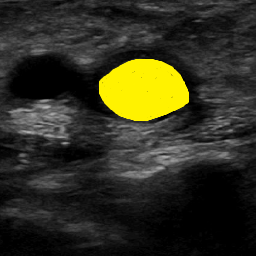
\includegraphics[scale= 0.7]{bab3/thrombus.png}
	\caption{Data Citra Ultrasound Gumpalan Darah}
	\label{fig:gumpalandarah}
\end{figure}

Data citra 2D \textit{ultrasound thrombus} menggunakan modalitas \textit{ultrasound} \textit{Telemed SmartUs EXT-1M} dan perangkat lunak \textit{Echowave II}. Fungsi dari modalitas \textit{ultrasound} \textit{Telemed SmartUs EXT-1M} adalah alat portable untuk mengakuisisi citra ultrasound guna melihat gambaran di dalam tubuh tanpa harus melakukan pembedahan. Echowave II merupakan perangkat lunak yang digunakan secara bersamaan dengan modalitas \textit{ultrasound} \textit{Telemed SmartUs EXT-1M} dan berfungsi untuk menangani pemrosesan data yang dikumpulkan oleh probe menjadi citra yang jelas dan dapat diinterpretasikan. Adapun modalitas Telemed SmartUs EXT-1M dapat dilihat pada Gambar \ref{Fig:tools_data_acquition} (a).

Kemudian, probe liniear dengan tipe L15-7L40H-5 digunakan dalam penelitian ini, yang menawarkan jangkauan frekuensi dari 7.5 hingga 15 MHz. Fungsi dari probe liniear itu sendiri adalah untuk mengirim gelombang suara ke dalam tubuh atau \textit{phantom} dimana gelombang ini akan dipantulkan kembali ke probe setelah mengenai struktur dalam tubuh, seperti pembuluh darah atau otot. Adapun \textit{probe liniear} dapat dilihat pada Gambar \ref{Fig:tools_data_acquition} (b). Untuk pengambilan posisi koordinat \textit{probe} dibutuhkan tiga marker yang akan terpasang pada \textit{probe}, kemudian dilacak menggunakan perangkat \textit{OpticTrack V120:Trio}. Koordinat yang dihasilkan oleh \textit{OpticTrack V120:Trio} akan dikalibrasi untuk memperoleh matriks transformasi. Matriks ini nantinya akan digunakan sebagai koordinat orientasi untuk citra rekonstruksi 3D. Adapun \textit{OpticTrack V120:Trio} dapat dilihat pada Gambar \ref{Fig:tools_data_acquition} (c). 

\begin{figure}[h]
        \centering
	\begin{tabular}{ll}
		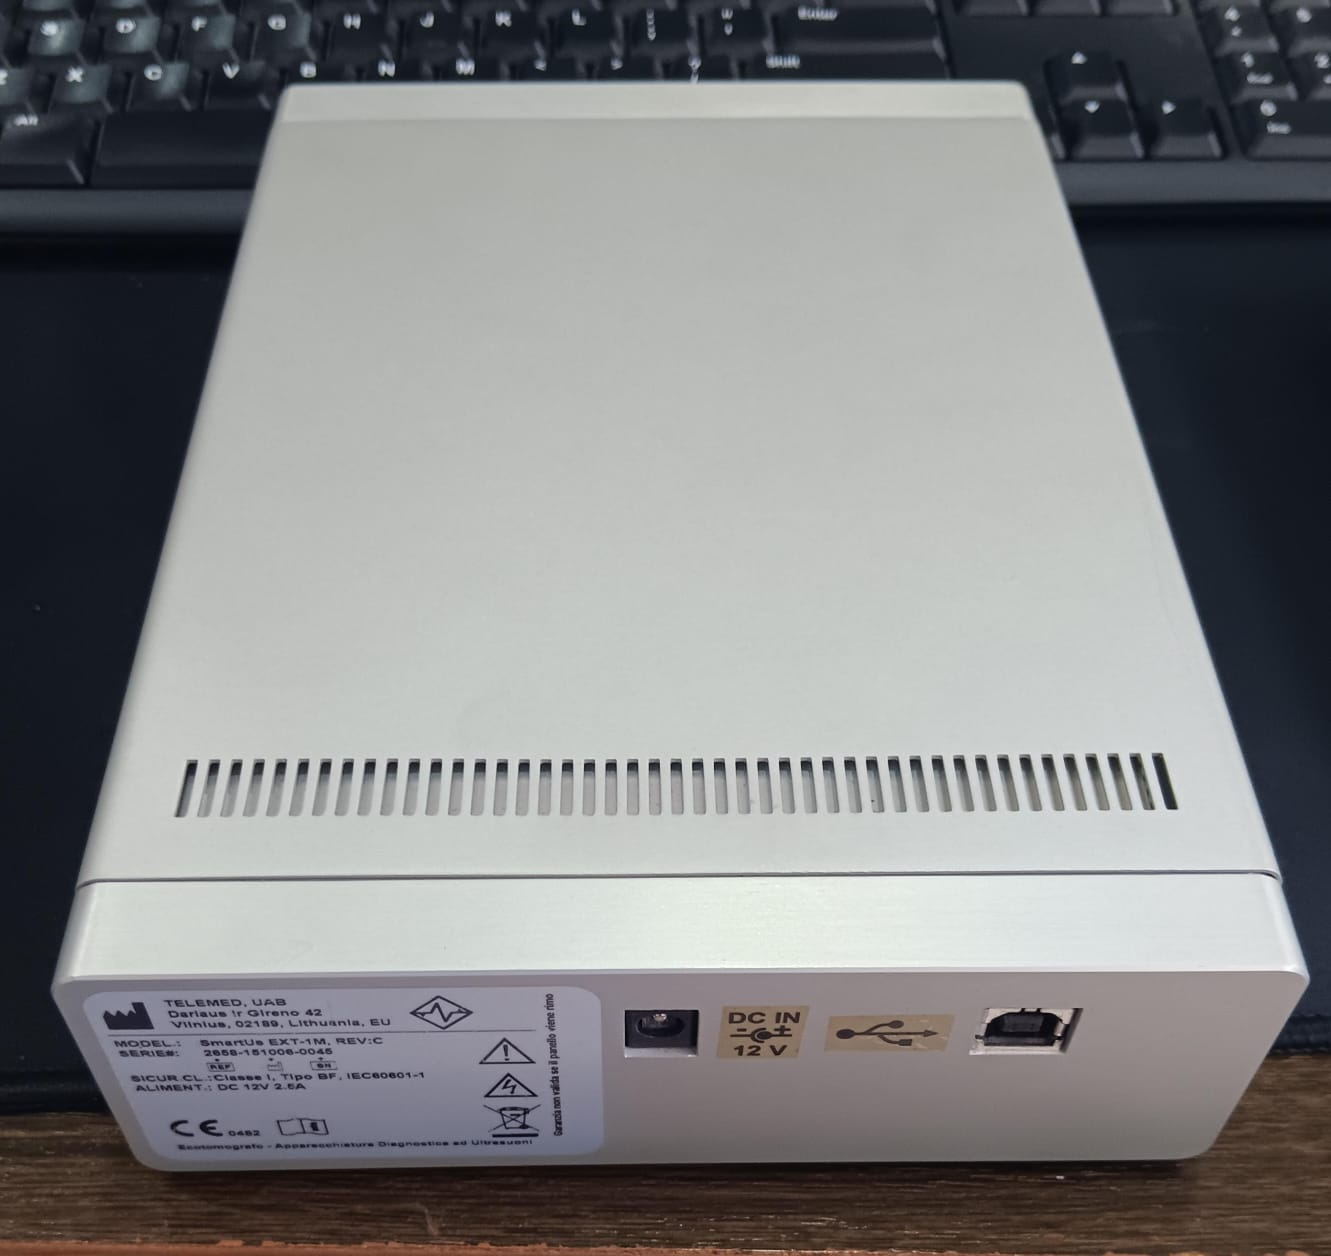
\includegraphics[scale=0.14]{bab3/usg_telemed.jpg}
		&
		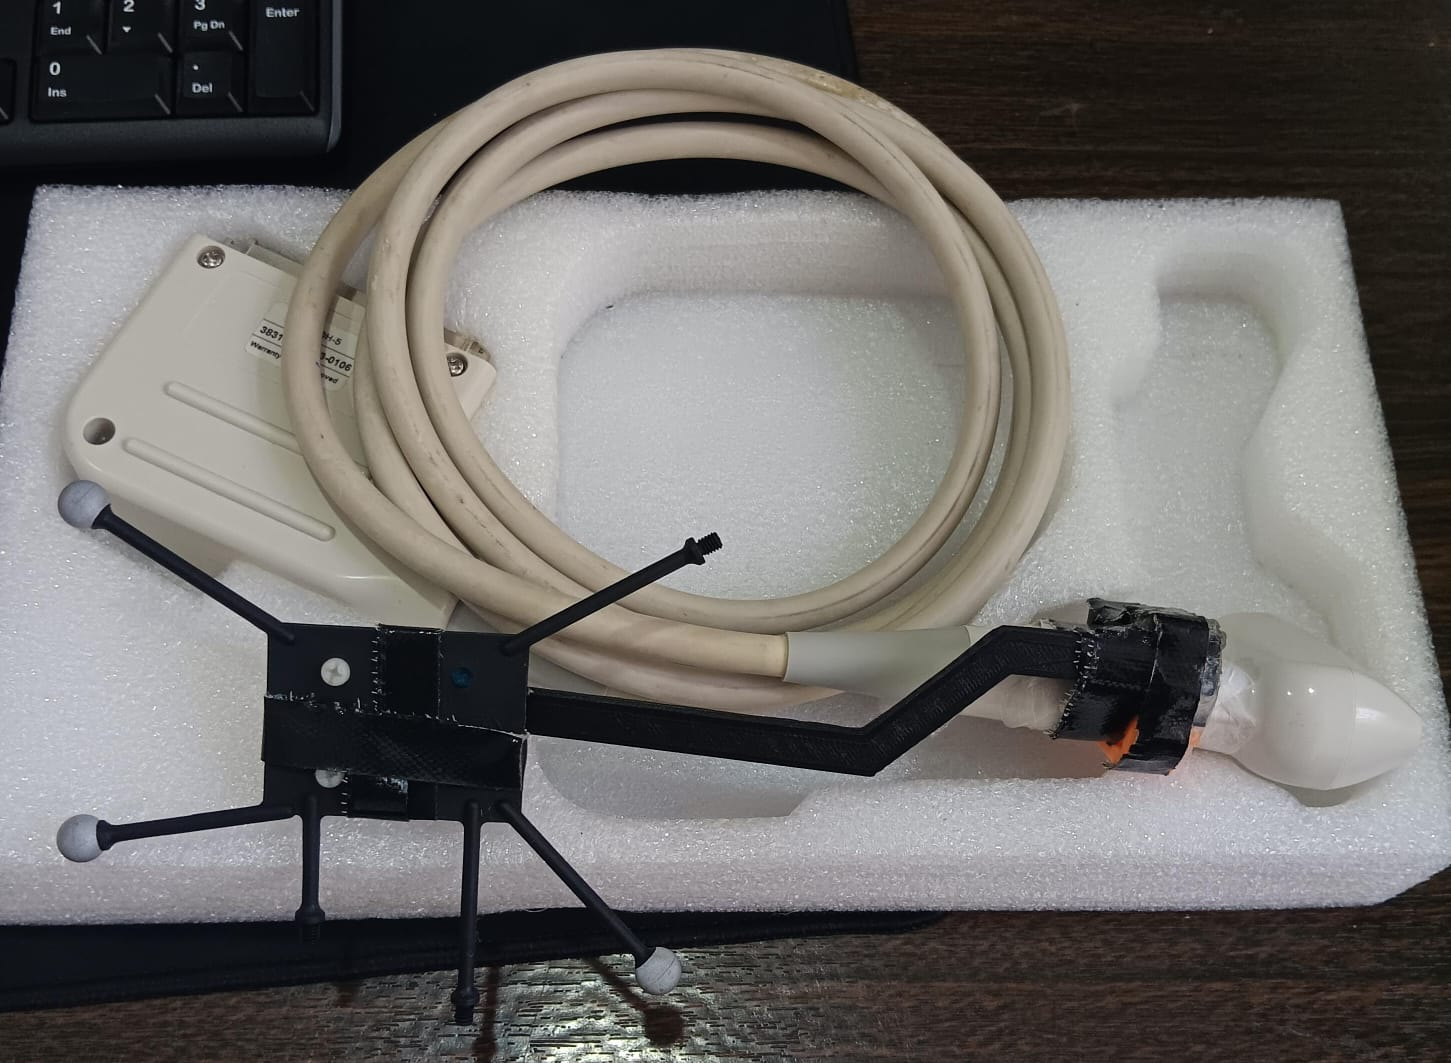
\includegraphics[scale=0.12]{bab3/probe_linear.jpg} \\
		\multicolumn{1}{c}{(a)} & \multicolumn{1}{c}{(b)} 
		
	\end{tabular}
	
	\begin{tabular}{ll}
		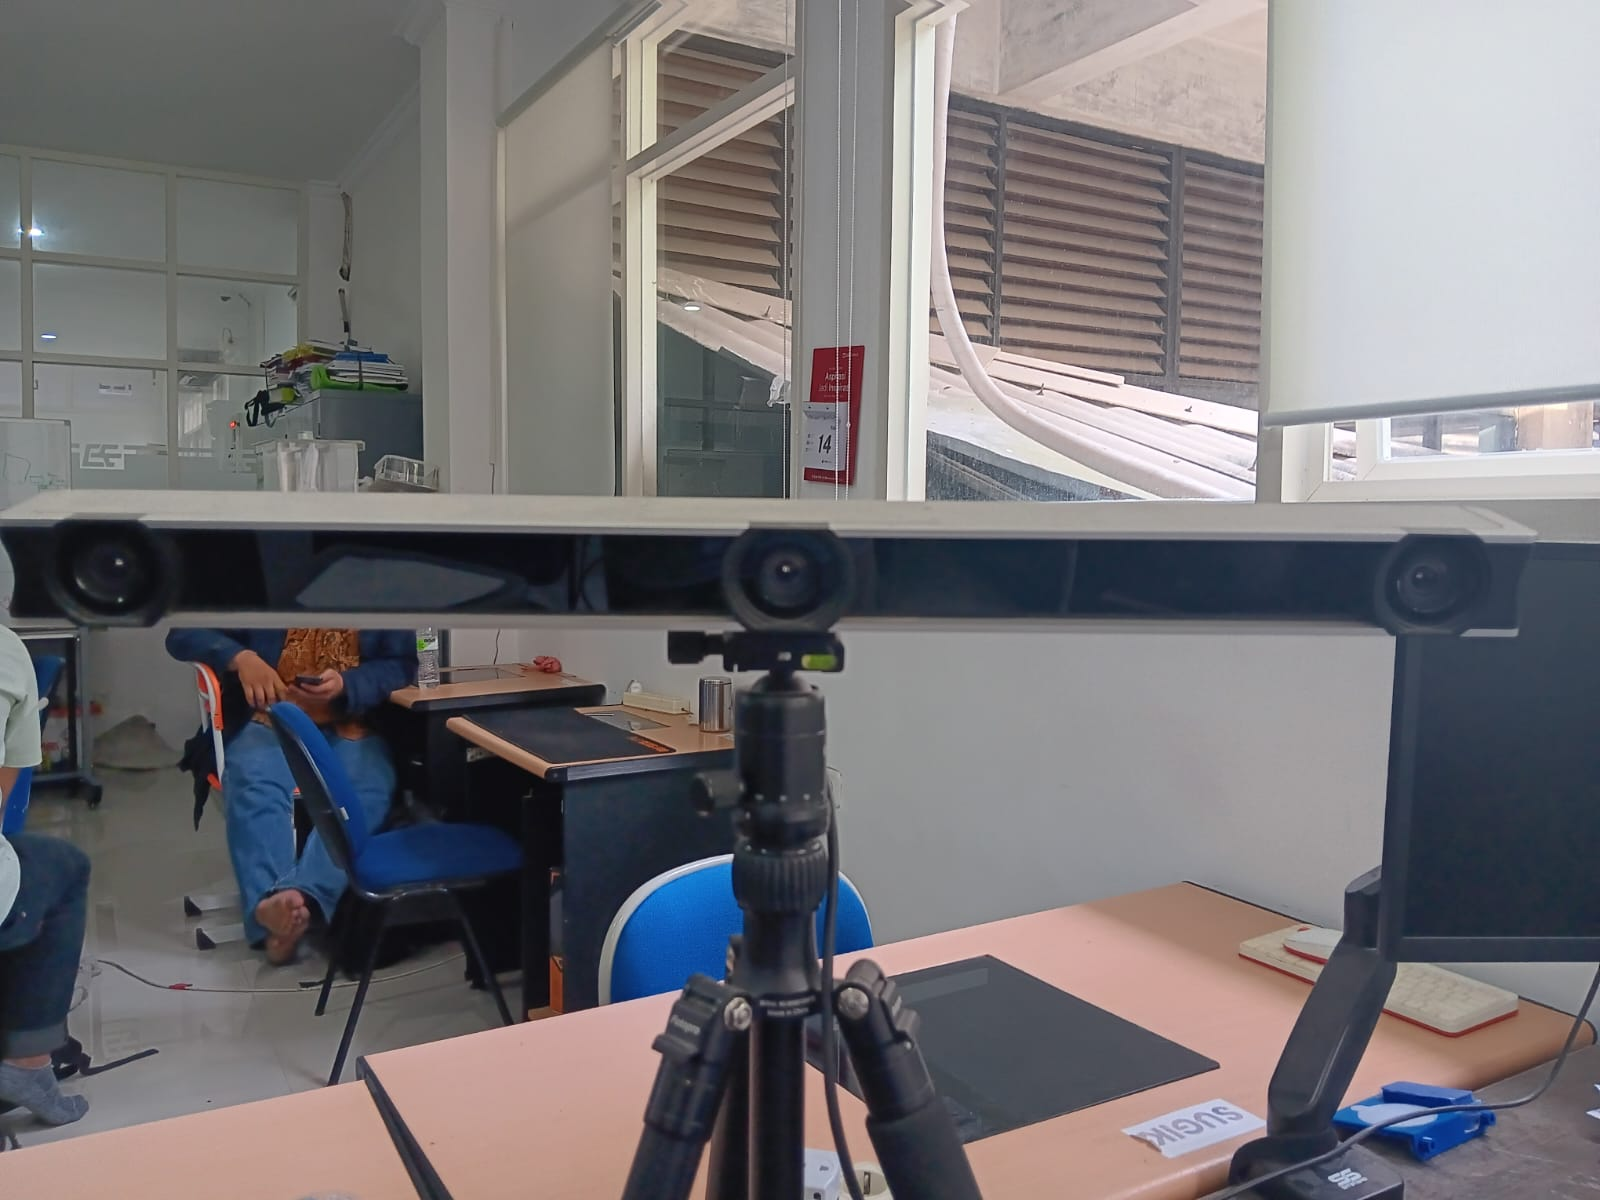
\includegraphics[scale=0.12]{bab3/img_optic_track.jpg}\\
		\multicolumn{1}{c}{(c)}  
		
	\end{tabular}
	\caption{(a) modalitas \textit{ultrasound} Telemed SmartUs EXT-1M, (b) Probe Linear, dan (c) perangkat \textit{OpticTrack V120:Trio}}
	\label{Fig:tools_data_acquition}
\end{figure}





\subsection{Prosedur Akuisisi Citra \textit{Ultrasound} Pembuluh Darah dan Gumpalan Darah Vena}
Prosedur akuisisi citra \textit{ultrasound} pembuluh darah dan gumpalan darah (\textit{thrombus}) vena membutuhkan perangkat  seperti \textit{probe} yang sudah terpasang marker, kamera \textit{optic track}, \textit{PC} yang digunakan untuk memproses dan memvisualkan citra, serta \textit{phantom} balon panjang. Akuisisi citra \textit{ultrasound thrombus} dilakukan dengan cara menempelkan permukaan \textit{probe} pada permukaan \textit{phantom} balon panjang. Fitur dan citra \textit{ultrasound thrombus} ditransformasikan ke dalam sistem koordinat marker yang terpasang pada pangkal \textit{probe} dan selanjutnya ditransformasikan ke dalam sistem koordinat kamera \textit{optic track} yang menjadi sistem koordinat global. Transformasi tersebut diperoleh dari hasil perhitungan jarak antara \textit{optic track} ke marker dan marker ke \textit{optic track}. 

%Konsep akuisisi data citra \textit{ultrasound} pembuluh darah dan \textit{thrombus} \textit{phantom} balon panjang dapat dilihat pada Gambar \ref{fig:prosedur_akuisisi}.
%
%\begin{figure}[H]
%	\centering
%	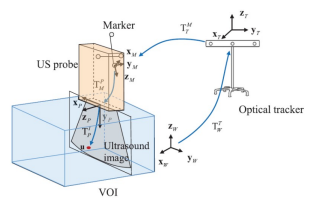
\includegraphics[scale= 0.7]{bab3/konsep_akuisisi_citra.png}
%	\caption{Konsep akuisisi data citra \textit{ultrasound} pembuluh darah dan \textit{thrombus} \textit{phantom} balon panjang}
%	\label{fig:prosedur_akuisisi}
%\end{figure}

Dalam proses akuisisi data menggunakan perangkat lunak dari hasil penelitian yang telah dilakukan sebelumnya. Perangkat lunak ini memiliki kemampuan untuk menyesuaikan tingkat kecerahan citra yang diperoleh, dapat mengatur frekuensi, kedalaman, dan titik fokus dari \textit{ultrasound}. Adapun antarmuka perangkat lunak yang digunakan untuk akuisisi citra 2D \textit{ultrasound thrombus} dapat dilihat pada Gambar. Proses akuisisi data menghasilkan citra 2D \textit{thrombus} pada pembuluh darah vena dengan dimensi 661 x 512 \textit{pixels} beserta data posisi marker yang berekstensi (\textit{.txt}). 


%Sebelum melakukan akuisisi citra, peneliti memastikan posisi marker yang terpasang pada pangkal \textit{probe} harus berhadapan dengan kamera \textit{optic track}. Hal itu bertujuan untuk memperoleh data posisi dari marker yang terpasang pada \textit{probe}. Data posisi marker diperoleh dari perhitungan jarak antara kamera \textit{optic track} ke marker dan marker ke kamera \textit{optic track}.    

% \subsection{Citra \textit{Ultrasound} Gumpalan Darah Vena}
% Data 2D citra USG gumpalan darah vena diperoleh dari data gumpalan darah lima pasien penderita DVT dengan total 317 citra. Gumpalan darah pasien terbentuk di dalam pembuluh darah vena bagian kaki. Data gumpalan darah ini menyajikan informasi visual yang dihasilkan dari pemindaian menggunakan sensor ultrasonografi (USG) yang memperlihatkan lokasi dan karakteristik gumpalan darah dalam pembuluh darah vena pada ke lima pasien tersebut. Data gumpalan darah ini penting untuk dianalisis guna membantu dokter dalam mendiagnosa, penilaian resiko, serta pengembangan metode pengobatan dan tindak lanjut untuk pasien penderita DVT.
% \begin{figure}[H]
% 	\centering
% 	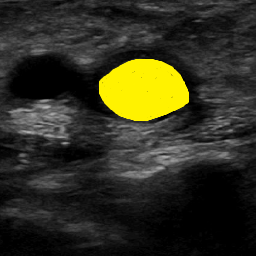
\includegraphics[scale= 0.7]{bab3/thrombus.png}
% 	\caption{Data Citra Ultrasound Gumpalan Darah}
% 	\label{fig:gumpalandarah}
% \end{figure}
%menggunakan peralatan seperti phantom, USG Telemed-SmartUs, dan Optitrack. Dalam proses pengambilan citra USG ini dilakukan dengan aturan dan ketentuan yang berlaku sebelum melakukan tahapan preprocessing.
%\subsection{Alat Pengambilan Citra}
%Penelitian ini menggunakan data ultrasound 2D gumpalan darah vena. Data citra gumpalan darah vena dikuisisi dari phantom yang merupakan replika dari bagian tubuh manusia. Phantom berbentuk gumpalan daging yang di dalamnya terdapat pembuluh darah beserta gumpalan darahnya. Pada penelitian ini Phantom akan menjadi sumber data utama simulasi gumpalan darah vena. Adapun phantom yang digunakan pada penelitian ini dapat dilihat pada Gambar 3.2.
%
%\begin{figure}[H]
%	\centering
%	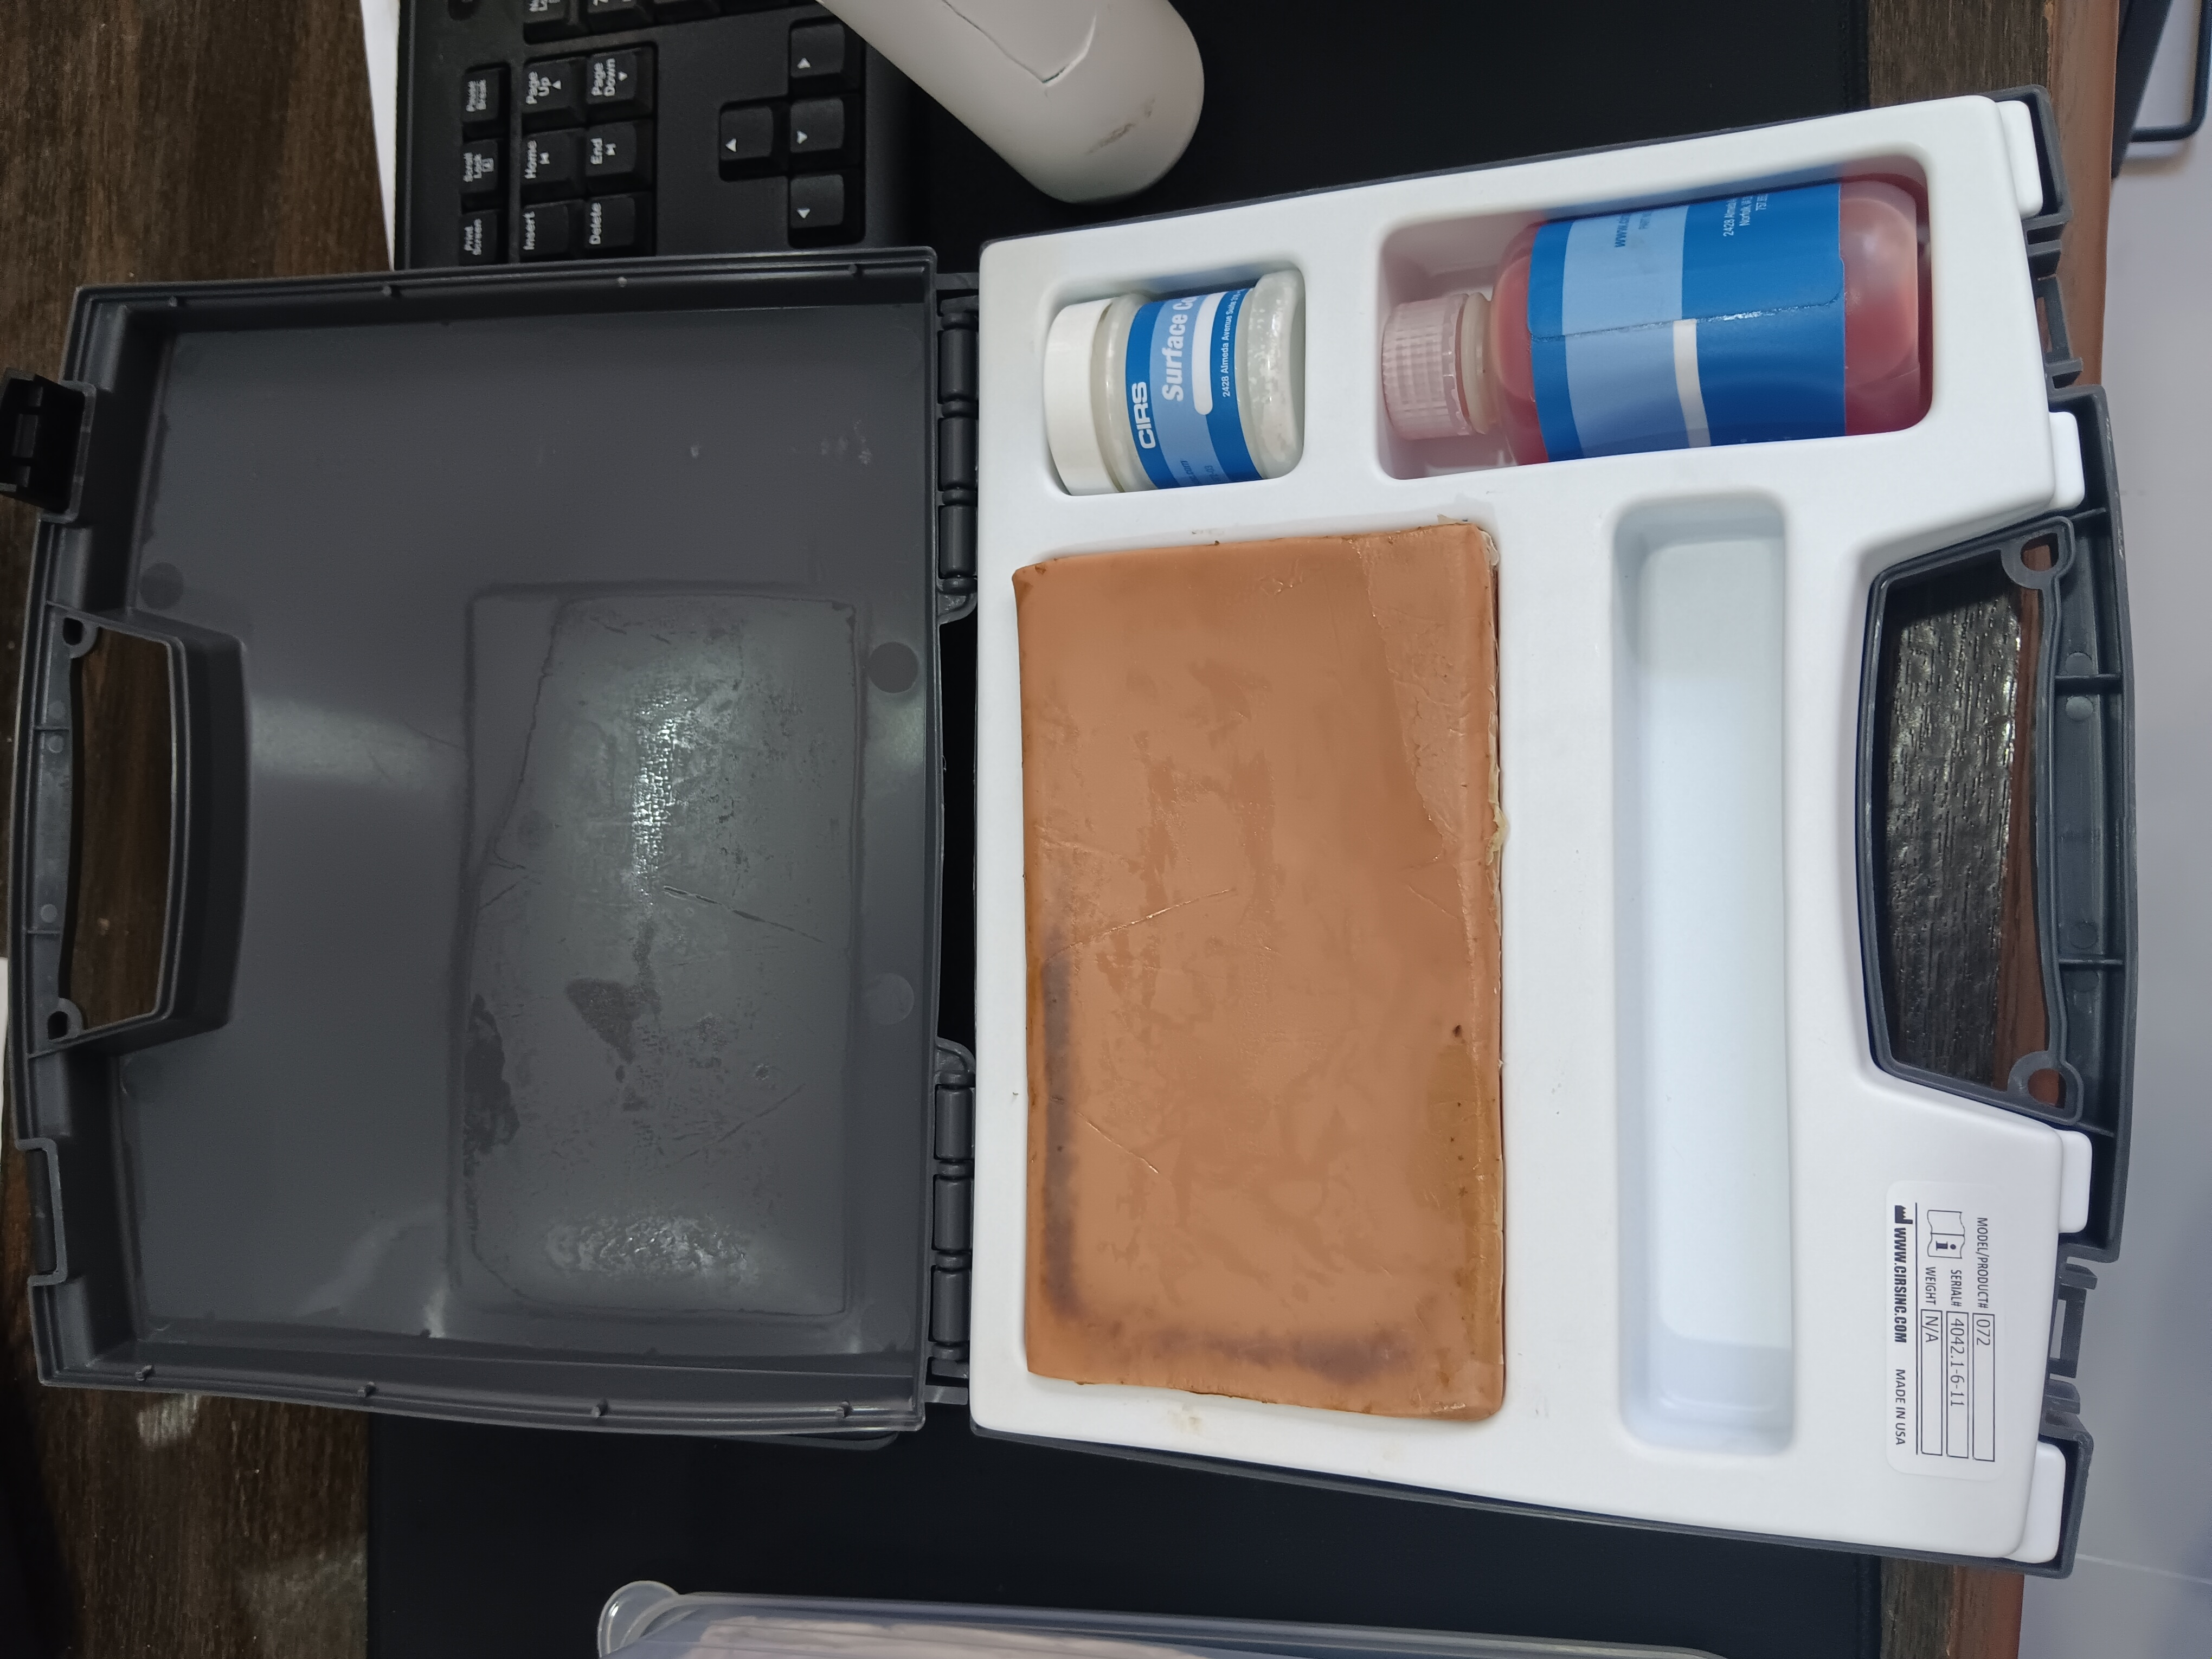
\includegraphics[width=\linewidth, angle=-90]{bab3/phantom.jpg}
%	\caption{Phantom}
%	\label{fig:phantom}
%\end{figure}
%
%Selain menggunakan phantom sebagai sumber data penelitian, peneliti akan menggunakan data gumpalan darah vena penderita DVT. Hal itu dilakukan agar dataset yang digunakan dalam proses pelatihan menggunakan model deep learning V-Net menjadi lebih bervariasi serta diharapkan mendapatkan hasil segmentasi area gumpalan darah vena yang akurat. 
%%adalah citra yang diperoleh dari kamera dengan ukuran $300\times 300$ dari beberapa sudut pandang yang berlainan.
%\subsection{Proses Pengambilan Citra}
\section{Preprocessing}
Citra 2D gumpalan darah (\textit{thrombus}) yang telah diakuisisi akan melalui dua langkah utama dalam tahap {\textit{preprocessing} sebelum masuk ke dalam proses \textit{training} menggunakan model \textit{deep learning} U-Net. Adapun tahap \textit{preprocessing} terbagi menjadi dua tahap yaitu rekonstruksi 3D citra \textit{ultrasound thrombus} dan mereduksi \textit{noise}. 
	
%normalisasi citra 2D \textit{ultrasound thrombus} dan mengubah bentuk 2D menjadi citra 3D \textit{thrombus}.

\subsection{Rekonstruksi 3D Citra \textit{Ultrasound} Pembuluh Darah dan Gumpalan Darah Vena}
\subsubsection{Penempatan Citra 2D \textit{Ultrasound} Pembuluh Darah dan Gumpalan Darah Vena pada Ruang \textit{Voxel} 3D}

%Penempatan setiap piksel citra \textit{ultrasound} pebuluh darah dan gumpalan darah \textit{thrombus} pada ruang \textit{voxel} 3D didasari oleh transformasi yang diperoleh pada proses kalibrasi. Ukuran ruang \textit{voxel} 3D ditentukan dengan cara mencari nilai batas nilai minimum dan nilai maksimum pada koordinat x,y, dan z. Batas tersebut didasari oleh posisi pada transformasi sistem koordinat pada ruang 3D.
Setelah dilakukan akuisisi data \textit{ultrasound} pembuluh darah dan gumpalan darah (\textit{thrombus}) \textit{phantom} balon panjang, setiap piksel citra tersebut ditempatkan pada ruang \textit{voxel} 3D berdasarkan transformasi yang diperoleh pada proses kalibrasi. Sebelum ditempatkan pada ruang \textit{voxel} 3D, harus dilakukan pembentukan ruang \textit{voxel} 3D terlebih dahulu. Proses pembuatan ruang \textit{voxel} disesuaikan dengan ukuran ruang \textit{voxel} yang dibutuhkan untuk penempatan hasil transformasi setiap citra \textit{ultrasound} pembuluh darah dan \textit{thrombus} \textit{phantom} balon panjang. Setiap piksel pada citra \textit{ultrasound} pembuluh darah dan \textit{thrombus} \textit{phantom} balon panjang ($f(u,v)$) dengan ukuran baris ($m$) dan kolom ($n$) akan ditempatkan pada voksel ($V(x,y,z)$). Adapun gambaran tentang penempatan citra \textit{ultrasound} pembuluh darah dan \textit{thrombus} \textit{phantom} balon panjang dapat dilihat pada Gambar \ref{fig:visualisasi_penempatan_voxel3d}. 

\begin{figure}[htbp]
	\centering
	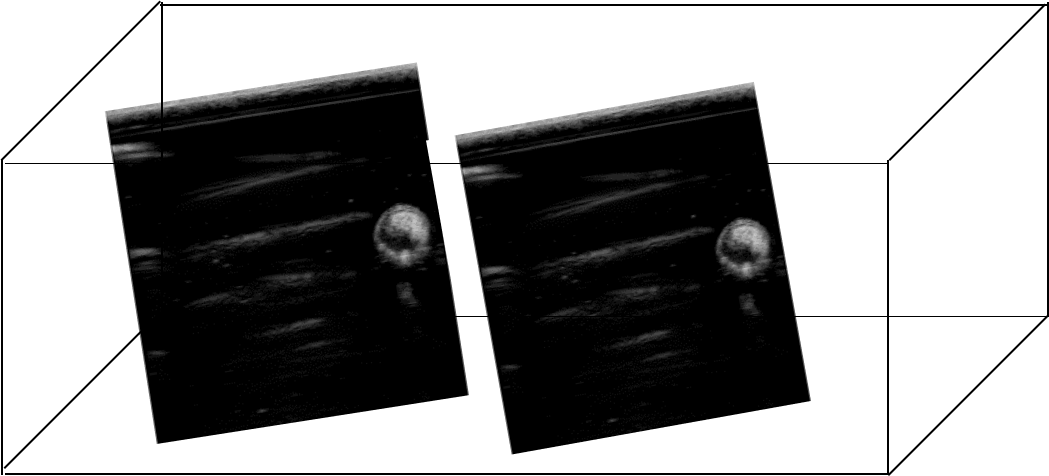
\includegraphics[scale= 0.3]{bab3/visualisasi_penempatan_voxel_3d.png}
	\caption{Visualisasi Penempatan Voxel 3D}
	\label{fig:visualisasi_penempatan_voxel3d}
\end{figure}

Adapun proses penempatan setiap piksel citra \textit{ultrasound} pada ruang \textit{voxel} 3D berdasarkan transformasi yang diperoleh pada proses kalibrasi dapat dirumuskan dengan Persamaan \ref{eq:transformasi-citra2d3d}. 

\begin{equation}
	\label{eq:transformasi-citra2d3d}
	V(x,y,z)\ =\ {_P^T}T\ \times{_U^P}T\ \ \times \begin{pmatrix}u \\v \\0 \\1\end{pmatrix}\
\end{equation}


Berdasarkan persamaan \ref{eq:transformasi-citra2d3d}, variabel \textit{V(x,y,z)} merupakan posisi \textit{voxel} yang merepresentasikan posisi data citra dalam ruang 3D. Variabel $_{P}^{T}T$  merupakan transformasi dari marker pada probe ultrasound ke pusat koordinat sistem kamera \textit{optictrack}. Variabel $_{U}^{P}T$  merupakan transformasi dari bidang citra \textit{ultrasound} ke marker pada \textit{probe ultrasound}. Variabel \textit{u} dan \textit{v} merupakan koordinat \textit{pixel} dari citra 2D. Adapun bagan proses penempatan piksel citra 2D \textit{ultrasound} pembuluh darah dan \textit{thrombus} \textit{phantom} balon panjang pada ruang \textit{voxel} 3D dengan kamera \textit{optic track} dapat dilihat pada Gambar \ref{fig:prosedur_rekonstruksi}.


\begin{figure}[htbp]
	\centering
	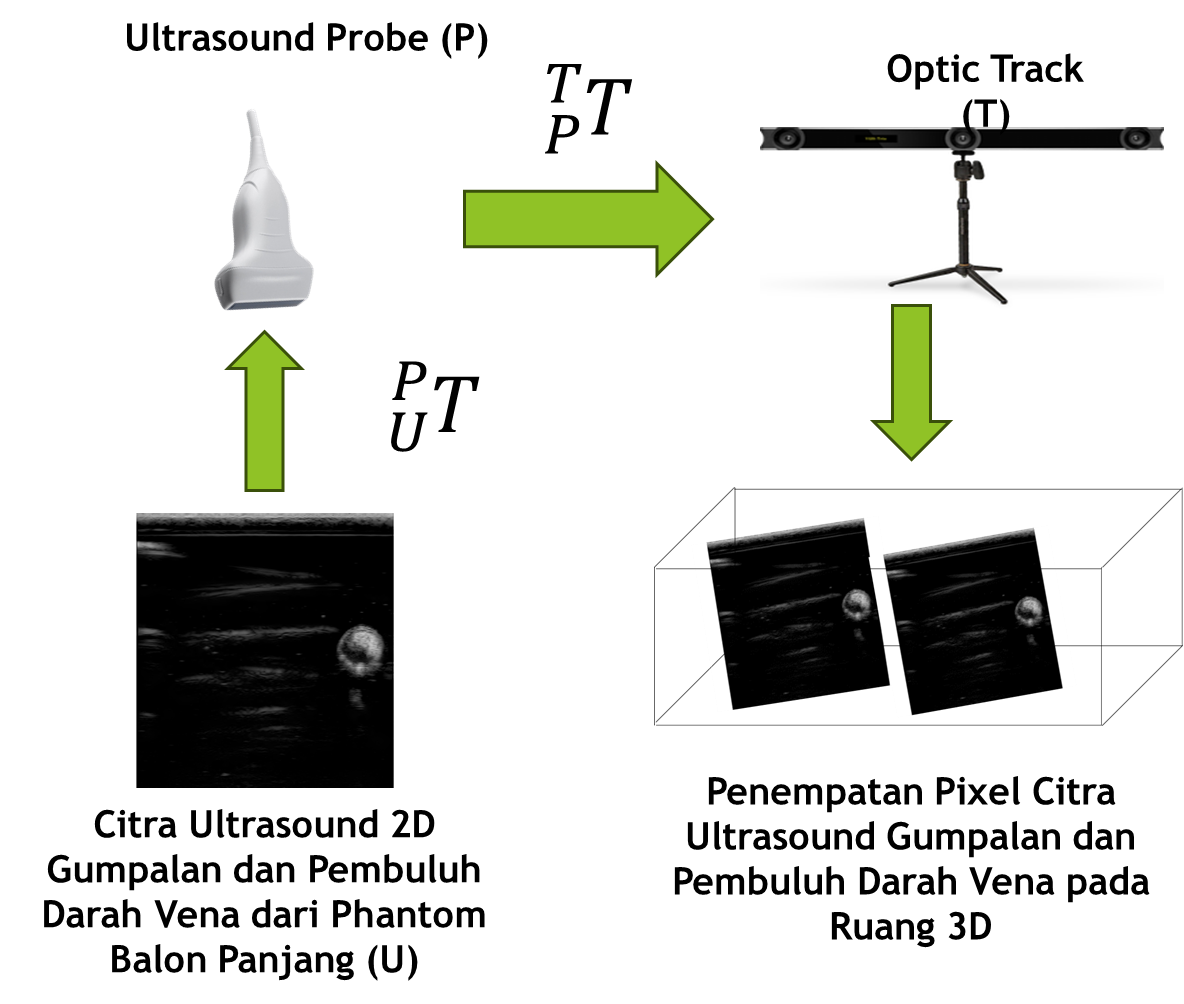
\includegraphics[scale= 0.25]{bab3/prosedur_rekonstruksi.png}
	\caption{Prosedur Rekonstruksi 3D}
	\label{fig:prosedur_rekonstruksi}
\end{figure}

Visualisasi hasil rekonstruksi 3D pada citra \textit{ultrasound} pembuluh darah dan \textit{thrombus} \textit{phantom} balon panjang menggunakan perangkat lunak \textit{3D slicer}. Hasil visualisasi tersebut dapat dilihat pada Gambar \ref{fig:visualisasi_hasil_rekosntruksi}.

\begin{figure}[htbp]
	\centering
	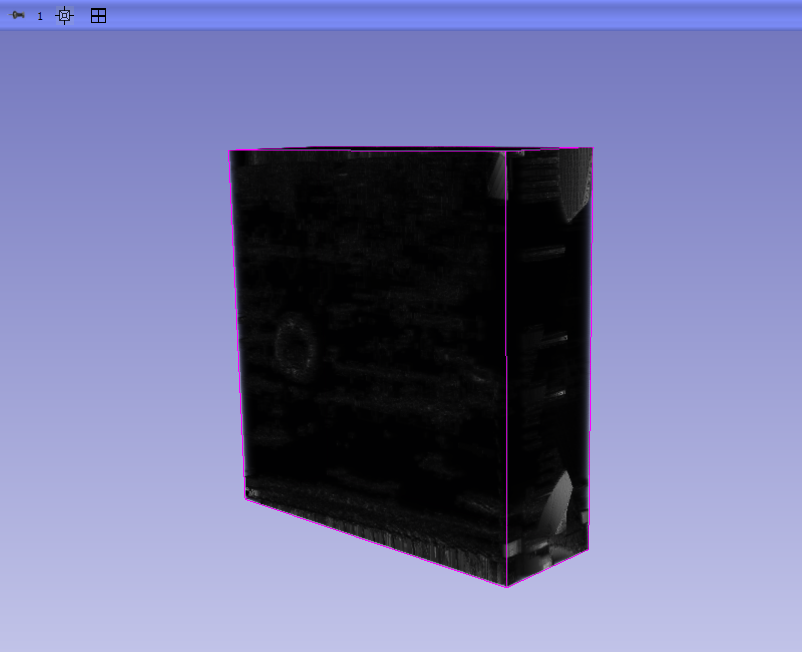
\includegraphics[scale= 0.5]{bab3/Hasil_Rekonstruksi_3d.png}
	\caption{Visualisasi hasil rekonstruksi 3D citra \textit{ultrasound} pembuluh darah dan \textit{thrombus} \textit{phantom} balon panjang menggunakan perangkat lunak \textit{3D Slicer}.}
	\label{fig:visualisasi_hasil_rekosntruksi}
\end{figure}




%\subsubsection{Visualisasi Hasil Rekonstruksi 3D Citra \textit{Ultrasound} Pembuluh Darah dan Gumpalan Darah Vena}


\subsection{Reduksi \textit{Noise}}
Pada penelitian ini data yang digunakan adalah data citra 3D \textit{ultrasound} pembuluh darah dan gumpalan darah (\textit{thrombus}) dari hasil rekonstruksi 3D serta data citra 2D \textit{ultrasound} \textit{thrombus} pada pembuluh darah vena penderita DVT (\textit{Deep Vein Thrombosis}). Citra \textit{ultrasound} \textit{thrombus} memiliki tingkat \textit{noise} yang tinggi. Oleh karena itu citra \textit{ultrasound thrombus} akan melalui tahap reduksi \textit{noise}. Khusus untuk citra 3D \textit{ultrasound} pembuluh darah dan gumpalan darah (\textit{thrombus}) dari hasil rekonstruksi 3D, agar mempermudah proses reduksi \textit{noise}, citra 3D tersebut di \textit{slice} menjadi citra 2D terlebih dahulu. Filter \textit{denoising} yang digunakan dalam penelitian ini yaitu filter \textit{gaussian}, filter \textit{median}, filter \textit{mean}, filter \textit{bilateral}, dan filter \textit{non local means}. Alasan peneliti memilih 5 filter \textit{denoising} tersebut dikarenakan ke lima filter \textit{denoising} tersebut sering digunakan dalam proses reduksi \textit{noise} citra biomedis. Filter \textit{gaussian} merupakan sebuah teknik dalam pengolahan citra yang digunakan untuk menghaluskan atau mengaburkan citra. Hal itu bertujuan untuk mengurangi detail - detail yang tidak diinginkan seperti \textit{noise} dalam sebuah citra. 
Filter \textit{gaussian} menggunakan operasi konvolusi, yaitu sebuah proses matematis dimana dapat menggabungkan 2 informasi. Informasi tersebut ialah citra asli dan sebuah matriks kernel. Kernel ini memiliki nilai - nilai tertentu yang membantu dalam reduksi \textit{noise}. Adapun filter \textit{gaussian} direpresentasikan dalam Persamaan \ref{eq:rumus_gaussian}.

\begin{equation}
	G\left(x,y\right)=\ e^\frac{{x^2+y}^2}{2\sigma^2}
	\label{eq:rumus_gaussian}
\end{equation}

Variabel $G(x,y)$ menunjukkan nilai filter \textit{gaussian} pada koordinat $(x,y)$ dalam ruang 2 dimensi. Variabel $e$ menunjukkan simpangan baku dari distribusi tersebut. Filter kedua yang digunakan dalam penelitian ini yaitu filter \textit{median}. Filter median merupakan salah satu filter yang paling umum digunakan dalam dunia biomedik. Operasi pada filter \textit{median} sangat sederhana yaitu dengan cara menggantikan nilai piksel tengah dengan nilai median dari piksel tetangganya. Perhitungan untuk mendapatkan hasil filter \textit{median} dapat dilihat pada Persamaan \ref{eq:rumus_median}.

\begin{equation}
	A(x,y) = median\left\{ f\left( x - i, y - i \right),i,j\in W  \right\}
	\label{eq:rumus_median}
\end{equation}

Dimana, variabel $W$ menunjukkan citra mask 2D, variabel $A(x,y)$ menunjukkan hasil output citra, dan variabel $f(x,y)$ menunjukkan citra asli. Filter ketiga yang digunakan dalam penelitian ini yaitu filter \textit{mean}. Filter \textit{mean} berfungsi untuk mengurangi \textit{noise} serta menghaluskan citra dengan memanfaatkan jumlah variasi intensitas minimal antara piksel yang berdekatan. Adapun filter \textit{mean} dapat dilihat pada Persamaan \ref{eq:rumus_mean}.

\begin{equation}
	f(x,y) = \frac{1}{mn}\sum_{(s,t)\epsilon S_{xy}}g(s,t)
	\label{eq:rumus_mean}
\end{equation}

Variable $f(x,y)$ menunjukkan nilai piksel hasil setelah proses penghalusan pada koordinat $(x,y)$ menggunakan filter \textit{mean}. Variabel $m$ dan $n$ menunjukkan jumlah baris dan kolom pada kernel. Variabel $g(s,t)$ menunjukkan nilai piksel pada koordinat $(s,t)$ sebelum penghalusan. Simbol sigma $\sum$ menunjukkan penjumlahan semua nilai piksel $g(s,t)$ di dalam kernel $S_{x,y}$. Filter yang keempat yan digunakan dalam penelitian ini yaitu filter \textit{bilateral}. Filter reduksi \textit{noise} \textit{bilateral} mempertimbangkan intensitas piksel berdasarkan lokasi piksel target maupun perbedaan jarak antar piksel. Berdasarkan hal tersebut, filter \textit{bilateral} efektif dalam mengurangi \textit{noise} citra tanpa mengaburkan tepi dan detail penting dalam citra. Adapun filter \textit{bilateral} dapat dilihat pada Persamaan \ref{eq:rumus_bilateral_1}. 


\begin{equation}\label{eq:rumus_bilateral_1}
	\begin{split}
		&I^{filtered}(x) = \frac{1}{W_p}\sum_{x_i\in\Omega}I\left(x_i\right)f_r(\parallel I\left(x_i\right) - I\left(x\right)\parallel)\\&g_s(\parallel \left(x_i\right)-x \parallel)
	\end{split}
\end{equation}


\begin{equation}
	{W_p}=\sum_{x_i\in\Omega}f_r(\parallel I\left(x_i\right) - I\left(x\right)\parallel)g_s(\parallel \left(x_i\right)-x \parallel)
	\label{eq:rumus_bilateral_2}
\end{equation}

Dimana, $W_p$ merupakan normalisasi. Variabel $I^{filtered}$ merepresentasikan citra yang telah difilter. Variabel $x$ merepresentasikan koordinat dari piksel saat ini yang digunakan untuk difilter. Variabel $I$ mewakili citra asli. Variabel $f_r$ merepresentasikan perubahan kernel untuk intensitas penghalusan. Variabel $g_s$ menunjukkan kernel abstraksi untuk menghaluskan fluktuasi koordinat. Kemudian filter reduksi \textit{noise} yaitu filter \textit{non local means}. Filter \textit{denoising} ini dirancang untuk menjaga informasi citra sekaligus menghilangkan \textit{noise} pada citra. Adapun perhitungan filter \textit{non local means} dapat dilihat pada Persamaan \ref{eq:rumus_nlm}.

\begin{equation} \label{eq:rumus_nlm}
	\begin{split}
		&NLM\mid I(m)\mid =\sum_{n\epsilon N_m}\omega(N_m,\ N_n)I(n)\\ &\left(\omega(N_m,\ N_n) = \frac{1}{Z\left(m\right)^{\mathcal{e}^\frac{-d}{h^2}}}\right)
	\end{split}    
\end{equation}

Dimana, variabel $I(n)$ merepresentasikan intensitas \textit{noise}. Variabel $\omega(N_m,\ N_n)$ merepresentasikan jumlah perbedaan antara piksel target dan piksel sekitarnya. Variabel $Z(m)$ merepresentasikan konstanta  normalisasi. Serta variabel $d$ menunjukkan jarak \textit{euclidean}. Adapun hasil reduksi \textit{noise} citra \textit{ultrasound thrombus} dan pembuluh darah \textit{phantom} balon panjang dan citra \textit{thrombus} pasien penderita DVT dapat dilihat pada Gambar \ref{fig:hasil_denoising_rekonstruksi} dan Gambar \ref{fig:hasil_denoising_ori}.

\begin{figure}[htbp]
	\centering
	\begin{tabular}{ccc}
			% Baris pertama dengan tiga gambar
			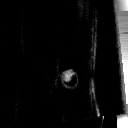
\includegraphics[width=0.3\textwidth]{bab3/reduksi_noise/img_360_ori.png} &
			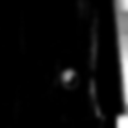
\includegraphics[width=0.3\textwidth]{bab3/reduksi_noise/img_360_gaussian.png} &
			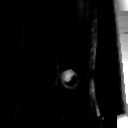
\includegraphics[width=0.3\textwidth]{bab3/reduksi_noise/img_360_median.png} \\
			(a)  & (b)  & (c)  \\ % Caption untuk baris pertama
			% Baris kedua dengan tiga gambar
			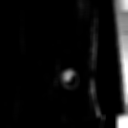
\includegraphics[width=0.3\textwidth]{bab3/reduksi_noise/img_360_mean.png} &
			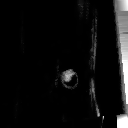
\includegraphics[width=0.3\textwidth]{bab3/reduksi_noise/img_360_bilateral.png} &
			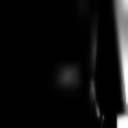
\includegraphics[width=0.3\textwidth]{bab3/reduksi_noise/img_360_nlm.png} \\
			(d)  & (e)  & (f)  % Caption untuk baris kedua
		\end{tabular}
	\caption{Hasil reduksi \textit{noise} citra \textit{ultrasound} pembuluh darah dan \textit{thrombus} \textit{phantom} balon panjang menggunakan filter sebagai berikut (a) tidak menggunakan filter; (b) filter \textit{gaussian}; (c) filter \textit{median}; (d) filter \textit{mean}; (e) filter \textit{bilateral}; (f) filter \textit{non-local means}}
	\label{fig:hasil_denoising_rekonstruksi}
\end{figure}


\begin{figure}[h]
	\centering
	\begin{tabular}{ccc}
		% Baris pertama dengan tiga gambar
		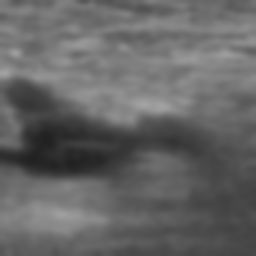
\includegraphics[width=0.3\textwidth]{bab4/citra-asli.jpg} &
		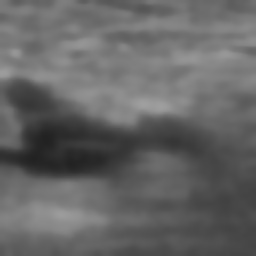
\includegraphics[width=0.3\textwidth]{bab4/citra-bilateral.jpg} &
		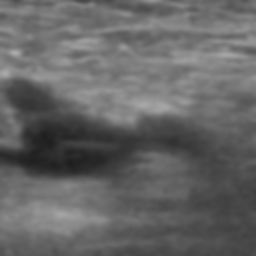
\includegraphics[width=0.3\textwidth]{bab4/citra-gaussian.jpg} \\
		(a)  & (b)  & (c)  \\ % Caption untuk baris pertama
		% Baris kedua dengan tiga gambar
		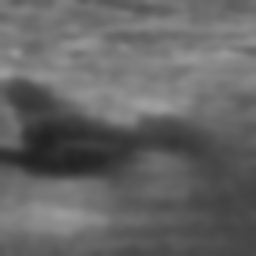
\includegraphics[width=0.3\textwidth]{bab4/citra-mean.jpg} &
		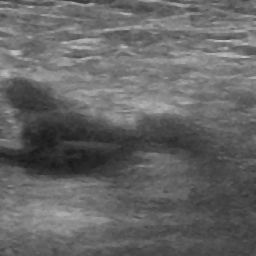
\includegraphics[width=0.3\textwidth]{bab4/citra-median.jpg} &
		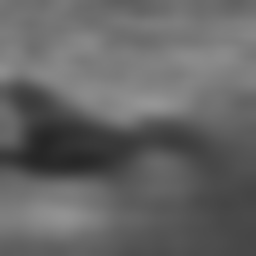
\includegraphics[width=0.3\textwidth]{bab4/citra-nlm.jpg} \\
		(d)  & (e)  & (f)  % Caption untuk baris kedua
	\end{tabular}
	\caption{Hasil reduksi \textit{noise} citra \textit{ultrasound} \textit{phantom} balon panjang menggunakan filter sebagai berikut (a) tidak menggunakan filter; (b) filter \textit{bilateral}; (c) filter \textit{gaussian}; (d) filter \textit{mean}; (e) filter \textit{median}; (f) filter \textit{non-local means}}
	\label{fig:hasil_denoising_ori}
\end{figure}

Citra 2D \textit{ultrasound} pembuluh darah dan \textit{thrombus} yang telah melalui tahapan reduksi \textit{noise} akan dilakukan pembuatan \textit{groundtruth} dengan menggunakan perangkat lunak \textit{Label Studio}. Perangkat lunak \textit{Label Studio} bersifat \textit{open source} yang tersedia melalui \textit{Python Package Index} (PyPI). Alasan peneliti memilih perangkat lunak \textit{Label Studio} karena perangkat lunak \textit{open source} ini dapat dioperasikan secara lokal dan mendukung berbagai jenis model anotasi dengan output yang diinginkan. Proses \textit{labelling} pada citra \textit{ultrasound} 2D ini menggunakan anotasi masking area untuk dua kelas yaitu \textit{multiclass semantic segmentation}. Metode ini menghasilkan citra hitam putih dimana area pembuluh darah vena dan \textit{thrombus} ditandai denga warna putih. Sementara itu, area lain yang diinterpretasikan sebagai bukan area pembuluh darah vena dan \textit{thrombus} ditandai dengan warna hitam.Citra hasil anotasi biasa disebut dengan citra \textit{mask}. Citra \textit{mask} ini kemudian diunduh dalam format file .PNG. Adapun proses pembuatan citra \textit{mask} dapat dilihat pada Gambar \ref{fig:label-studio}.

\begin{figure}[htbp]
	\centering
	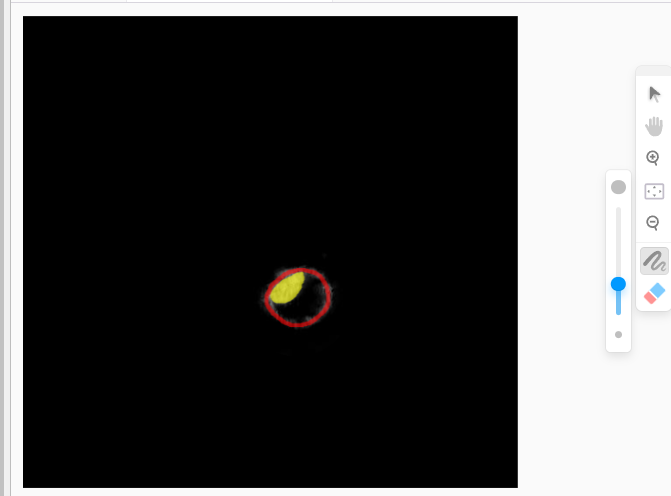
\includegraphics[scale= 0.25]{bab3/label-studio.png}
	\caption{Proses Pembuatan Citra Mask Menggunakan \textit{Label Studio}}
	\label{fig:label-studio}
\end{figure}

\begin{figure}[htbp]
	\centering
	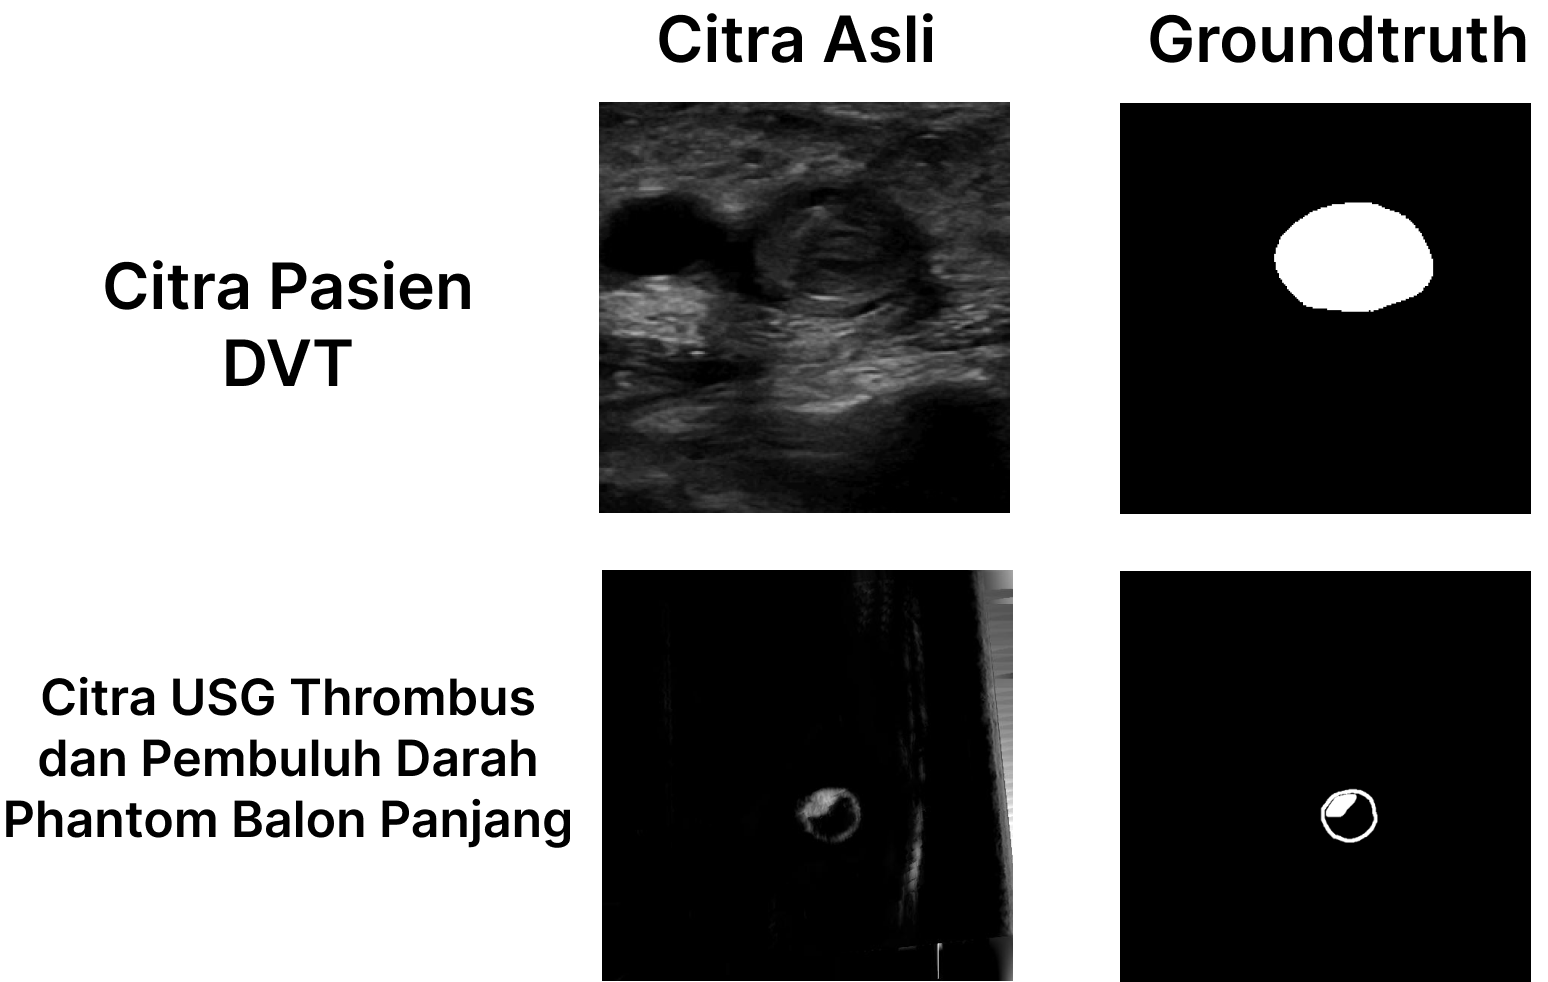
\includegraphics[scale= 0.15]{bab3/Hasil-Label.png}
	\caption{Proses Pembuatan Citra Mask Menggunakan \textit{Label Studio}}
	\label{fig:result-label}
\end{figure}

%Citra pembuluh darah dan gumpalan darah \textit{thrombus} yang telah direkonstruksi menjadi bentuk 3D, seringkali mengandung \textit{noise} yang tinggi yang dapat mengganggu interpretasi dan analisis lebih lanjut. Oleh karena itu, citra 3D akan diubah menjadi citra 2D melalui proses \textit{slicing} untuk mempermudah dalam proses reduksi \textit{noise}.
%
%Proses reduksi \textit{noise} pada citra \textit{ultrasound} pembuluh darah dan \textit{thrombus} ini sangat penting. Keberadaan \textit{noise} dapat menyebabkan kesalahan dalam menginterpretasi citra dan mempengaruhi keakuratan diagnosa. Langkah pertama pada proses reduksi \textit{noise} pada citra \textit{ultrasound} pembuluh darah dan \textit{thrombus} hasil rekonstruksi yaitu menggunakan teknik \textit{Hough Transform} yang merupakan sebuah metode dalam OpenCV yang efektif untuk mendeteksi bentuk geometris berupa lingkaran. \textit{Hough Transform} digunakan untuk mengidentifikasi dan menandai area dalam citra \textit{ultrasound} yang sesuai dengan bentuk lingkaran. Bentuk lingkaran merupakan karakteristik dari pembuluh darah pada citra.
%
%Setelah berhasil mengidentifikasi lingkaran menggunakan metode \textit{Hough Transform}, langkah berikutnya yaitu memisahkan objek lingkaran beserta objek yang berada di dalam radius lingkaran tersebut dari bagian lainnya dalam citra. Hal ini dilakukan dengan cara menggelapkan area di sekitar lingkaran, yaitu dengan membuat bagian luar dari radius lingkaran menjadi hitam. Langkah ini membantu dalam meningkatkan fokus pada area pembuluh darah dan \textit{thrombus}, sekaligus menghilangkan elemen - elemen lain yang menambah \textit{noise} pada citra. Dengan demikian, proses ini tidak hanya mengurangi \textit{noise} tetapi juga dapat memudahkan analisis dan interpretasi citra \textit{ultrasound} pembuluh darah dan \textit{thrombus} dengan lebih jelas dan akurat. Adapun hasil reduksi noise dapat dilihat pada Gambar \ref{fig:comparison-denoising}.
%
%
%\begin{figure}[htbp]
%	\centering
%	\begin{tabular}{ccc}
%		\textbf{Citra Asli} & \textbf{Denoising} \\
%		% Baris pertama dengan tiga gambar
%		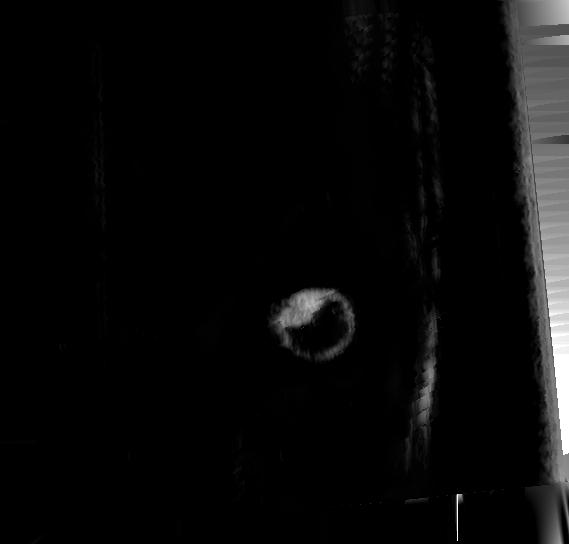
\includegraphics[scale=0.3]{bab3/citra-asli-rekonstruksi.jpg} &
%		\includegraphics[scale=0.3]{bab3/citra-asli-denoising-rekonstruksi.png} & \\
%		(a) & (b)    % Caption untuk baris pertama
%		% Caption untuk baris kedua
%	\end{tabular}
%	\caption{(a) Citra asli dan (b) Citra hasil \textit{denoising}}
%	\label{fig:comparison-denoising}
%\end{figure}  

%Sementara itu, citra 2D \textit{ultrasound} \textit{thrombus} yang diperoleh dari pasien penderita DVT akan melalui tahap reduksi \textit{noise}. Filter \textit{denoising} yang digunakan dalam penelitian ini yaitu filter \textit{gaussian}, filter \textit{median}, filter \textit{mean}, filter \textit{bilateral}, dan filter \textit{non local means}. Alasan peneliti memilih 5 filter \textit{denoising} tersebut dikarenakan ke lima filter \textit{denoising} tersebut sering digunakan dalam proses reduksi \textit{noise} citra 2D biomedis. 

%Citra 2D \textit{ultrasound} pembuluh darah dan \textit{thrombus} dari \textit{slicing} citra 3D hasil rekonstruksi dan pasien penderita DVT yang telah melalui tahapan reduksi \textit{noise} akan dilakukan pembuatan \textit{groundtruth} dengan menggunakan perangkat lunak \textit{Label Studio}. Perangkat lunak \textit{Label Studio} bersifat \textit{open source} yang tersedia melalui \textit{Python Package Index} (PyPI). Alasan peneliti memilih perangkat lunak \textit{Label Studio} karena perangkat lunak \textit{open source} ini dapat dioperasikan secara lokal dan mendukung berbagai jenis model anotasi dengan output yang diinginkan. Proses \textit{labelling} pada citra \textit{ultrasound} 2D ini menggunakan anotasi masking area untuk dua kelas yaitu \textit{multiclass semantic segmentation}. Metode ini menghasilkan citra hitam putih dimana area pembuluh darah vena dan \textit{thrombus} ditandai denga warna putih. Sementara itu, area lain yang diinterpretasikan sebagai bukan area pembuluh darah vena dan \textit{thrombus} ditandai dengan warna hitam.Citra hasil anotasi biasa disebut dengan citra \textit{mask}. Citra \textit{mask} ini kemudian diunduh dalam format file .PNG. Adapun proses pembuatan citra \textit{mask} dapat dilihat pada Gambar \ref{fig:label-studio}.
%
%\begin{figure}[htbp]
%	\centering
%	\includegraphics[scale= 0.2]{bab3/label-studio.png}
%	\caption{Proses Pembuatan Citra Mask Menggunakan \textit{Label Studio}}
%	\label{fig:label-studio}
%\end{figure}
%
%\begin{figure}[htbp]
%	\centering
%	\includegraphics[scale= 0.1]{bab3/Hasil-Label.png}
%	\caption{Proses Pembuatan Citra Mask Menggunakan \textit{Label Studio}}
%	\label{fig:result-label}
%\end{figure}


Kemudian, khusus untuk citra 2D \textit{ultrasound} pembuluh darah dan \textit{thrombus} dari hasil \textit{slicing} citra 3D hasil rekonstruksi beserta citra \textit{mask}nya akan disusun kembali menjadi bentuk 3D berdasarkan urutan waktunya. Penyusunan kembali menjadi bentuk 3D ini digunakan untuk proses \textit{training} untuk membuat model segmentasi 3D. 

 
 

% \subsection{Menghapus Noise}
% Sebelum melakukan proses training data menggunakan model deep learning, citra 2D USG gumpalan darah pasien penderita DVT akan melalui proses menghapus \textit{noise}. Citra USG memiliki \textit{noise} yang tinggi. Sehingga pada penelitian ini dilakukan tahap peningkatan kualitas citra menggunakan filter \textit{gaussian}. Alasan memilih filter gaussian yang Pada penelitian ini karena berdasarkan penelitian sebelumnya, filter gaussian mampu mengurangi \textit{noise} secara detail serta membantu meningkatkan optimasi hasil segmentasi. Hasil citra 2D USG gumpalan darah yang telah melalui tahap penghapusan \textit{noise} dengan menggunakan filter \textit{gaussian}, akan melalui tahap pelabelan \textit{ground truth} area gumpalan darah.

% \subsection{Pelabelan \textit{Ground Truth} Area \textit{Thrombus}}
% Pelabelan \textit{ground truth} area citra gumpalan darah (\textit{thrombus}) digunakan sebagai citra label pada proses \textit{training} menggunakan model \textit{deep learning} U-Net. Tujuan utama pelabelan citra adalah untuk mengenali dan membedakan objek atau area yang berbeda dalam citra tersebut. Proses pelabelan pada penelitian ini menggunakan aplikasi \textit{label studio} yang bersifat \textit{open source}. Proses pelabelan area gumpalan darah vena pada citra 2D \textit{ultrasound} memberi label \textit{masking} pada area gumpalan darah. Hasil dari pelabelan tersebut menghasilkan citra \textit{mask} yang berwarna hitam putih. Warna hitam pada citra \textit{mask} menandakan bahwa bukan termasuk area gumpalan darah. Sedangkan warna putih pada citra \textit{mask} menandakan area gumpalan darah. Kemudian hasil pelabelan akan disimpan menjadi file citra baik format .PNG, .JPG, .Tiff, dan lain - lain. Adapun hasil pelabelan citra 2D gumpalan darah \textit{ultrasound} dari pasien penderita DVT dapat dilihat pada Gambar \ref{fig:labelling}. 

% \begin{figure}[H]
% 	\centering
% 	\includegraphics[scale= 0.6]{bab3/label.png}
% 	\caption{Hasil Pelabelan Citra 2D USG Gumpalan Darah Vena}
% 	\label{fig:labelling}
% \end{figure}

% digunakan sebagai dataset pelatihan (\textit{training}) dengan menggunakan model U-Net. 
%\section{Model V-Net}
%Model V-Net dapat digunakan dalam proses segmentasi guna membantu dalam identifikasi posisi gumpalan darah yang akurat. Data yang digunakan dalam proses training menggunakan model V-Net adalah hasil preprocessing citra 3D USG gumpalan darah yang telah dilakukan sebelumnya.
%\subsection{Fitur Warna}
%\lipsum[1]
%\subsection{Fitur Permukaan}
\section{Segmentasi Gumpalan Darah}
Pada tahap utama segmentasi gumpalan darah vena terdapat tiga tahapan yaitu (1) \textit{training} menggunakan model \textit{deep learning} U-Net; (2) ekstraksi fitur citra input pada \textit{encoder} U-Net; dan (3) segmentasi gumpalan darah vena pada \textit{decoder} U-Net.

\subsection{Pembagian Data Sebelum Segmentasi}
Pada proses pelatihan (\textit{training}) menggunakan 2 data citra \textit{ultrasound} yaitu citra 3D \textit{ultrasound} pembuluh darah dan \textit{thrombus} phantom balon panjang dari hasil rekosntruksi dan citra 2D \textit{thrombus} lima pasien penderita DVT. Citra 3D \textit{ultrasound} pembuluh darah dan \textit{thrombus} phantom balon panjang dari hasil rekosntruksi dapat dilakukan segementasi dengan 2 cara yaitu segmentasi 2D dan 3D. Untuk melakukan segmentasi 2D, data citra 3D \textit{ultrasound} pembuluh darah dan \textit{thrombus} phantom balon panjang dari hasil rekonstruksi akan di \textit{slice} menjadi citra 2D. Jumlah citra 3D \textit{ultrasound} yang digunakan untuk proses \textit{training} yaitu berjumlah 4 citra. Kemudian jumlah citra 2D hasil \textit{slice} citra 3D \textit{ultrasound} pembuluh darah dan \textit{thrombus} phantom balon panjang berjumlah 389 citra. Sedangkan jumlah citra 2D \textit{ultrasound} \textit{thrombus} pasien DVT berjumlah 312 citra. 

Sebelum proses pelatihan data dilakukan, ketiga citra tersebut akan dibagi menjadi dua jenis data yaitu data pelatihan (\textit{train}) dan data validasi (\textit{validation}). Data \textit{train} merupakan bagian terbesar dari dataset yang digunakan untuk melatih model. Semakin banyak data \textit{train} yang berkualitas dan bervariasi, semakin baik model segmentasi dapat mempelajari karakteristik yang lebih kompleks. Kemudian data \textit{validation} merupakan data yang digunakan untuk mengevaluasi kinerja model segemntasi selama proses pelatihan (\textit{training}). Hal tersebut bertujuan untuk memeriksa apakah model segmentasi mengalami \textit{overfitting}. Data \textit{validation} harus berbeda dari data \textit{train} tetapi masih mewakili distribusi yang sama. Adapun pembagian data citra 3D \textit{ultrasound} pembuluh darah dan \textit{thrombus} \textit{phantom} balon panjang dari hasil rekonstruksi mengacu pada Tabel \ref{tab:pembagian_data_citra_3d_rekonstruksi}.

% Please add the following required packages to your document preamble:
% \usepackage{graphicx}
\begin{table}[htbp]
	\centering
	\caption{Pembagian data citra 3D \textit{ultrasound} pembuluh darah dan \textit{thrombus} \textit{phantom} balon panjang}
	\label{tab:pembagian_data_citra_3d_rekonstruksi}
	\resizebox{\textwidth}{!}{%
		\renewcommand{\arraystretch}{2.0} % Menyesuaikan tinggi baris (1 adalah default, nilai yang lebih besar untuk lebih banyak ruang)
		\setlength{\tabcolsep}{10pt} % Menyesuaikan padding horizontal (nilai default biasanya 6pt)
		\begin{tabular}{|l|l|c|c|}
			\hline
			\multicolumn{1}{|c|}{\textbf{Pembagian}} & \multicolumn{1}{c|}{\textbf{Deskripsi}}             & \textbf{Jumlah} & \textbf{Rasio} \\ \hline
			\textbf{Data pelatihan}                  & Bagian data yang digunakan untuk melatih model      & 4               & 80\%           \\ \hline
			\textbf{Data validasi}                   & Bagian data yang digunakan untuk mengevaluasi model & 1               & 20\%           \\ \hline
		\end{tabular}%
	}
\end{table}

Kemudian, pembagian data citra 2D hasil \textit{slice} citra 3D \textit{ultrasound} pembuluh darah dan \textit{thrombus} \textit{phantom} balon panjang dari hasil rekonstruksi mengacu pada Tabel \ref{tab:pembagian_data_citra_2d_rekonstruksi}

\begin{table}[htbp]
	\centering
	\caption{Pembagian data citra 2D hasil \textit{slice} citra 3D \textit{ultrasound} pembuluh darah dan \textit{thrombus} \textit{phantom} balon panjang}
	\label{tab:pembagian_data_citra_2d_rekonstruksi}
	\resizebox{\textwidth}{!}{%
		\renewcommand{\arraystretch}{2.0} % Menyesuaikan tinggi baris (1 adalah default, nilai yang lebih besar untuk lebih banyak ruang)
		\setlength{\tabcolsep}{10pt} % Menyesuaikan padding horizontal (nilai default biasanya 6pt)
		\begin{tabular}{|l|l|c|c|}
			\hline
			\multicolumn{1}{|c|}{\textbf{Pembagian}} & \multicolumn{1}{c|}{\textbf{Deskripsi}}             & \textbf{Jumlah} & \textbf{Rasio} \\ \hline
			\textbf{Data pelatihan}                  & Bagian data yang digunakan untuk melatih model      & 310               & 80\%           \\ \hline
			\textbf{Data validasi}                   & Bagian data yang digunakan untuk mengevaluasi model & 79               & 20\%           \\ \hline
		\end{tabular}%
	}
\end{table}

Pembagian data citra 2D \textit{ultrasound} \textit{thrombus} pasien penderita DVT mengacu pada Tabel \ref{tab:pembagian_data_citra_2d_ori}

\begin{table}[htbp]
	\centering
	\caption{Pembagian data citra 2D \textit{ultrasound} \textit{thrombus} pasien penderita DVT.}
	\label{tab:pembagian_data_citra_2d_ori}
	\resizebox{\textwidth}{!}{%
		\renewcommand{\arraystretch}{2.0} % Menyesuaikan tinggi baris (1 adalah default, nilai yang lebih besar untuk lebih banyak ruang)
		\setlength{\tabcolsep}{10pt} % Menyesuaikan padding horizontal (nilai default biasanya 6pt)
		\begin{tabular}{|l|l|c|c|}
			\hline
			\multicolumn{1}{|c|}{\textbf{Pembagian}} & \multicolumn{1}{c|}{\textbf{Deskripsi}}             & \textbf{Jumlah} & \textbf{Rasio} \\ \hline
			\textbf{Data pelatihan}                  & Bagian data yang digunakan untuk melatih model      & 250               & 80\%           \\ \hline
			\textbf{Data validasi}                   & Bagian data yang digunakan untuk mengevaluasi model & 62               & 20\%           \\ \hline
		\end{tabular}%
	}
\end{table} 

%Model V-Net dapat digunakan dalam proses segmentasi guna membantu dalam identifikasi posisi gumpalan darah yang akurat. Data yang digunakan dalam proses training menggunakan model V-Net adalah hasil reduksi noise citra 3D USG gumpalan darah yang telah dilakukan sebelumnya. Output dari prediksi model V-Net adalah citra mask pada area gumpalan darah pada pembuluh darah vena. Pada arsitektur V-Net terdiri dari bagian kiri dan kanan jaringan. Penggabungan bagian kiri dan kanan pada model V-Net dalam pembuatan prediksi hasil segmentasi citra dengan cara mengeksrak fitur dari citra input dan mengubah fitur tersebut menjadi hasil prediksi yang spesifik dengan memperbesar ukuran citra. 
\subsection{Training Deep Learning Model U-Net}
Pada penelitian ini model U-Net dipilih oleh peneliti guna melakukan segmentasi area gumpalan darah (\textit{thrombus}) pada pembuluh darah vena. Proses pelatihan (\textit{training}) dalam kasus segmentasi citra menggunakan model \textit{deep learning} seperti U-Net adalah untuk mengajarkan model tersebut bagaimana mengidentifikasi dan membedakan objek target dimana dalam kasus peneliti pada gumpalan darah (\textit{thrombus}) pada pembuluh darah vena. Dalam proses segmentasi, penelitian ini menggunakan bahasa pemrograman \textit{Python} versi 3 yang dijalankan melalui \textit{platform Google Colab}. Adapun spesifikasi \textit{platform Google Colab} dapat dilihat pada Tabel \ref{tab:spesifikasi_platform_google_colab}.


\begin{table}[htbp]
	\centering
	\caption{Spesifikasi platform Google Colab}
	\label{tab:spesifikasi_platform_google_colab}
	\resizebox{\textwidth}{!}{%
		\renewcommand{\arraystretch}{2.0} % Menyesuaikan tinggi baris (1 adalah default, nilai yang lebih besar untuk lebih banyak ruang)
		\setlength{\tabcolsep}{10pt}
		\begin{tabular}{|l|l|}
			\hline
			\textbf{CPU}         & AMD EPYC 7B12 (2,24 GHz) \\ \hline
			\textbf{GPU}         & Tesla T4                 \\  \hline
			\textbf{RAM}         & 12,7 GB                  \\  \hline
			\textbf{Penyimpanan} & 166,8 GB                 \\ \hline
		\end{tabular}%
	}
\end{table}

Dalam proses \textit{training} juga ada beberapa konfigurasi yang didefinisikan oleh peneliti. Adapun konfigurasi pelatihan yang didefinisikan oleh peneliti mengacu pada Tabel \ref{tab:konfigurasi_hiperparameter_model}.


\begin{table}[htbp]
	\centering
	\caption{Konfigurasi Hiperparameter Model}
	\label{tab:konfigurasi_hiperparameter_model}
	\resizebox{\textwidth}{!}{%
		\renewcommand{\arraystretch}{2.0} % Menyesuaikan tinggi baris (1 adalah default, nilai yang lebih besar untuk lebih banyak ruang)
		\setlength{\tabcolsep}{10pt}
		\begin{tabular}{|l|l|}
			\hline
			\textbf{Batch Size}                           & 8                   \\ \hline
			\textbf{Epoch}                                & 100                 \\ \hline
			\textbf{Tingkat Pembelajaran (Learning Rate)} & 0,0001              \\ \hline
			\textbf{Pengoptimalan (Optimizer)}            & Adam                \\ \hline
			\textbf{Loss}                                 & Binary Crossentropy \\ \hline
			\textbf{Aktivasi Layer}                       & Softmax             \\ \hline
			\textbf{Kelas}                                & 2                   \\ \hline
		\end{tabular}%
	}
\end{table}

Hasil segmentasi akan dievaluasi menggunakan 5 \textit{metric} evaluasi sebagai berikut (1)\textit{accuracy}; (2)\textit{loss}; (3)\textit{Intersection over Union} (IoU); (4)\textit{dice coefficient}; dan (5) \textit{hausdorff distance}. \textit{Metric} evaluasi \textit{accuracy} berfungsi untuk menghitung nilai prediksi yang tepat terhadap data yang memiliki area gumpalan darah \textit{thrombus} pada pembuluh darah vena yang diperoleh melalui model segmentasi U-Net pada saat proses \textit{training}. Nilai persentase \textit{accuracy} yang tinggi menunjukkan bahwa model yang dihasilkan lebih akurat dalam melakukan segmentasi citra \textit{ultrasound} \textit{thrombus}.

Metrik evaluasi \textit{loss} berfungsi untuk menghitung nilai kesalahan model segmentasi dalam memprediksi data citra yang memiliki area \textit{thrombus} pada saat proses \textit{training}. Nilai \textit{loss} yang rendah menunjukkan nilai kesalahan yang kecil antara citra prediksi dan \textit{groundtruth} dari citra \textit{ultrasound thrombus}. Metrik evaluasi \textit{Intersection over Union (IoU)} berfungsi untuk mengukur kemiripan antara dua objek dalam citra. Dalam kasus pada penelitian ini, pengukuran kemiripan antara \textit{ground truth} dari citra \textit{ultrasound} \textit{thrombus} dan citra prediksi \textit{thrombus} yang dihasilkan melalui proses segmentasi. Nilai IoU memiliki rentang 0 hingga 1. Apabila nilai IoU mendekati 0, maka citra hasil prediksi segmentasi tidak mirip dengan bentuk dari \textit{groundtruth}. Sedangkan jika nilai IoU mendekati 1, maka citra hasil prediksi segmentasi mirip dengan bentuk dari \textit{groundtruth}. \textit{Metric} evaluasi \textit{dice coefficient} memiliki fungsi yang sama dengan \textit{metric} evaluasi IoU yaitu mengukur kemiripan antara dua objek dalam citra. \textit{Dice coefficient} memiliki rentang 0 hingga 1. \textit{Dice coefficient} dipilih peneliti karena sensitivitasnya terhadap perubahan kecil dalam area segmentasi. Nilai \textit{hausdroff distance} diperoleh melalui perhitungan nilai 2 titik terjauh pada 2 citra. Di dalam penelitian ini, \textit{haudorff distance} diterapkan pada pengukuran antara \textit{groundtruth} dan hasil prediksi segmentasi. Nilai \textit{hausdorff distance} akan bernilai 0 jika himpunan kedua titik (\textit{groundtruth} dan hasil prediksi segmentasi) memiliki kesamaan. Sedangkan apabila nilai \textit{hausdorff distance} memiliki nilai yang tinggi, maka himpunan kedua titik (\textit{groundtruth} dan hasil prediksi segmentasi) tersebut memiliki jarak yang berjauhan. Hasil uji performa kedua model tersebut akan dijelaskan pada Bab 4.
%Pembagian data pada proses \textit{training}, Seluruh data dibagi sebesar 80\% yang digunakan untuk data \textit{train} sedangkan sebesar 20\% akan digunakan sebagai data \textit{validation}. Data \textit{train} berjumlah 254 citra serta data \textit{validation} berjumlah 63 citra.

%Matriks evaluasi pada penelitian ini menggunakan \textit{Intersection over Union} (IoU Score). Metode IoU score memiliki beberapa karakteristik yang sesuai dengan kebutuhan evaluasi model segmentasi dengan karakteristik sebagai berikut:

%\begin{enumerate}
%    \item Intuitif: Nilai IoU adalah persentase \textit{overlap} antara area objek yang sebenarnya dan area yang dihasilkan oleh model segmentasi. Ini mudah dipahami dan mudah digunakan untuk mengevaluasi kinerja model segmentasi.
%    \item Fleksibel : Nilai IoU dapat digunakan untuk berbagai jenis bentuk dari citra itu sendiri. Seperti objek persegi, lingkaran, atau poligon
%    \item \textit{Robust} : Nilai IoU digunakan untuk menghitung luas overlap antara area objek sebenarnya dan area yang dihasilkan oleh model segmentasi. 
%    \item Konsisten : Nilai IoU digunakan untuk memberikan konsistensi dalam mengevaluasi kinerja model segmentasi
%    \item Memperhitungkan false positive dan false negative
%\end{enumerate}

%Jumlah nilai IoU yang lebih tinggi menunjukkan bahwa sistem segmentasi bekerja dengan baik dalam menemukan objek dalam citra. Proses pengukuran IoU terdiri dari menghitung luas overlap antara area objek yang sebenarnya dan area yang dihasilkan oleh sistem segmentasi, lalu dibandingkan dengan luas total area objek yang sebenarnya dan area yang dihasilkan oleh sistem segmentasi.

\subsection{Ekstraksi Fitur Citra Input pada Encoder U-Net}
Pada penelitian ini dilakukan segmentasi 2D dan 3D menggunakan model U-Net. Pada arsitektur U-Net terdapat bagian \textit{encoder} dan \textit{decoder}. Model U-Net menggabungkan bagian \textit{encoder} dan \textit{decoder} untuk membuat prediksi segmen citra dengan mengekstrak fitur tersebut menjadi prediksi segmen yang lebih spesifik yang memperbesar ukuran citra. Pada segmentasi 2D, input citra 2D ultrasound akan melalui bagian \textit{encoder} model U-Net untuk proses ekstraksi fitur - fitur pada citra tersebut. Berikut ini ilustrasi citra input pada model U-Net2D dengan hasil output citra \textit{mask} area gumpalan darah dapat dilihat pada Gambar \ref{fig:modelU-Net2D}.

\begin{figure}[htbp]
	\centering
	\includegraphics[scale= 0.2]{bab3/unet_2d.png}
	\caption{Arsitektur U-Net 2D}
	\label{fig:modelU-Net2D}
\end{figure}

Masing - masing layer pada \textit{encoder} model U-Net akan mengimplementasikan filter \textit{convolutional} terhadap citra input. Kemudian citra input akan di \textit{pooling} sehingga ukuran dimensinya menjadi berkurang serta mengekstrak fitur yang lebih abstrak. Proses ini berlangsung hingga tahap akhir bagian \textit{encoder}. Fitur yang dihasilkan oleh \textit{encoder} akan digunakan sebagai input pada bagian \textit{decoder}. Pada bagian \textit{encoder} U-Net akan dilakukan uji coba modifikasi menggunakan model \textit{pre-trained} VGG16 untuk meningkatkan performa ekstraksi fitur citra input. Uji coba performa model \textit{pre-trained} VGG16 dan U-Net akan dibandingkan dengan model U-Net standar.

Kemudian pada segmentasi 3D, input citra 3D \textit{ultrasound} akan melalui bagian \textit{encoder} model U-Net3D untuk proses eksraksi fitur - fitur pada citra tersebut. Adapun yang membedakan dari model U-Net2D dan U-Net3D terletak pada inputan citranya, layer konvolusi, layer \textit{maxpooling}, serta layer \textit{transpose}. Pada model U-Net3D, inputan citra layer konvolusi, layer \textit{maxpooling}, serta layer \textit{transpose} semua dalam bentuk 3 dimensi. Berikut ini ilustrasi citra input pada model U-Net3D dengan hasil output citra \textit{mask} area gumpalan darah dapat dilihat pada Gambar \ref{fig:model_U-Net3D}.  

\begin{figure}[htbp]
	\centering
	\includegraphics[scale= 0.2]{bab3/Unet 3d.png}
	\caption{Arsitektur U-Net 3D}
	\label{fig:model_U-Net3D}
\end{figure}


Hasil performa segmentasi dari kedua model tersebut akan dievaluasi menggunakan 5 metrik evaluasi yaitu \textit{accuracy}, \textit{loss}, \textit{Intersection over Union} IoU, \textit{dice coefficient}, \textit{hausdorff distance}.

\subsection{Segmentasi Gumpalan Darah Vena pada \textit{Decoder} U-Net}
Kemudian output dari hasil ekstraksi pada bagian \textit{encoder} akan menjadi input pada bagian \textit{decoder} model U-Net. Pada bagian \textit{decoder} berfungsi untuk mengubah fitur dari bagian \textit{encoder} menjadi prediksi segmen citra. Bagian ini menggunakan layer \textit{transposed} untuk meningkatkan ukuran citra yang dihasilkan pada layer sebelumnya. Setiap layer pada bagian \textit{decoder} akan menggabungkan fitur dari layer sebelumnya guna membuat prediksi segmen area gumpalan darah (\textit{thrombus}). Proses ini dilakukan hingga layer terakhir bagian \textit{decoder}.

%\section{Visualisasi Gumpalan Vena 3D}
\section{Skenario Pada Penelitian}

Dalam rangka membuat model yang lebih efisien dan akurat untuk segmentasi gumpalan darah \textit(thrombus) vena pada citra \textit{ultrasound}, penelitian ini telah dirancang dengan lima skenario penelitian yang berbeda. Setiap skenario dikembangkan untuk mengeksplorasi dan menilai penggunaan model U-Net standar dan model \textit{pre-trained} VGG16 dan U-Net dalam konteks segmentasi 2D dan 3D. Skenario pada penelitian ini dapat dilihat pada Gambar \ref{fig:skenario_penelitian}.


\begin{figure}[htbp]
	\centering
	\includegraphics[scale= 0.2]{bab3/skenario_penelitian.png}
	\caption{Skenario Pada Penelitian}
	\label{fig:skenario_penelitian}
\end{figure}

Untuk data citra \textit{ultrasound} di setiap skenario pada segmentasi 2D akan dilakukan reduksi \textit{noise} dengan menggunakan 5 filter \textit{denoising} yaitu (1) filter \textit{gaussian}; (2) filter \textit{median}; (3) filter \textit{mean}; (4) filter \textit{bilateral}; dan (5) filter \textit{non local means}. Hasil pelatihan pada setiap skenario akan di evaluasi menggunakan 5 metrik evaluasi yaitu \textit{accuarcy}, \textit{loss}, \textit{IoU}, \textit{dice coefficient}, dan \textit{hausdorff distance}.


%\lipsum[4]
%\section{Segmentasi Gumpalan Darah}
%\lipsum[2]







	\cleardoublepage
	\chapter{HASIL DAN PEMBAHASAN}
% Please add the following required packages to your document preamble:
% \usepackage{multirow}
% \usepackage[table,xcdraw]{xcolor}
% If you use beamer only pass "xcolor=table" option, i.e. \documentclass[xcolor=table]{beamer}

% Please add the following required packages to your document preamble:
% \usepackage{multirow}
% \usepackage{graphicx}
% \usepackage[table,xcdraw]{xcolor}
% If you use beamer only pass "xcolor=table" option, i.e. \documentclass[xcolor=table]{beamer}
%\begin{table}[H]
%\centering
%\caption{Rencana Penelitian}
%\label{tab:researchPlan}
%\resizebox{\textwidth}{!}{%
%\begin{tabular}{|l|llllllllllllllll|}
%\hline
%\multicolumn{1}{|c|}{\cellcolor[HTML]{FFFFFF}}                                         & \multicolumn{16}{c|}{Minggu ke-}                                                                                                                                                                                                                                                                                                                                                                                                                                                                                                                                                                                                                                                                                                                                                                                                                                     \\ \cline{2-17} 
%\multicolumn{1}{|c|}{\multirow{-2}{*}{\cellcolor[HTML]{FFFFFF}Kegiatan}}               & \multicolumn{1}{l|}{1}                                               & \multicolumn{1}{l|}{2}                                               & \multicolumn{1}{l|}{3}                                               & \multicolumn{1}{l|}{4}                                               & \multicolumn{1}{l|}{5}                        & \multicolumn{1}{l|}{6}                        & \multicolumn{1}{l|}{7}                        & \multicolumn{1}{l|}{8}                        & \multicolumn{1}{l|}{9}                        & \multicolumn{1}{l|}{10}                       & \multicolumn{1}{l|}{11}                       & \multicolumn{1}{l|}{12}                       & \multicolumn{1}{l|}{13}                       & \multicolumn{1}{l|}{14}                       & \multicolumn{1}{l|}{15}                       & 16                       \\ \hline
%Studi literatur                                                                        & \multicolumn{1}{l|}{\cellcolor[HTML]{FCFF2F}{\color[HTML]{FCFF2F} }} & \multicolumn{1}{l|}{\cellcolor[HTML]{FCFF2F}{\color[HTML]{FCFF2F} }} & \multicolumn{1}{l|}{\cellcolor[HTML]{FCFF2F}{\color[HTML]{FCFF2F} }} & \multicolumn{1}{l|}{\cellcolor[HTML]{FCFF2F}{\color[HTML]{FCFF2F} }} & \multicolumn{1}{l|}{}                         & \multicolumn{1}{l|}{}                         & \multicolumn{1}{l|}{}                         & \multicolumn{1}{l|}{}                         & \multicolumn{1}{l|}{}                         & \multicolumn{1}{l|}{}                         & \multicolumn{1}{l|}{}                         & \multicolumn{1}{l|}{}                         & \multicolumn{1}{l|}{}                         & \multicolumn{1}{l|}{}                         & \multicolumn{1}{l|}{}                         &                          \\ \hline
%\begin{tabular}[c]{@{}l@{}}Menghapus noise citra 2D \\ USG gumpalan darah\end{tabular} & \multicolumn{1}{l|}{}                                                & \multicolumn{1}{l|}{}                                                & \multicolumn{1}{l|}{}                                                & \multicolumn{1}{l|}{}                                                & \multicolumn{1}{l|}{\cellcolor[HTML]{FCFF2F}} & \multicolumn{1}{l|}{}                         & \multicolumn{1}{l|}{}                         & \multicolumn{1}{l|}{}                         & \multicolumn{1}{l|}{}                         & \multicolumn{1}{l|}{}                         & \multicolumn{1}{l|}{}                         & \multicolumn{1}{l|}{}                         & \multicolumn{1}{l|}{}                         & \multicolumn{1}{l|}{}                         & \multicolumn{1}{l|}{}                         &                          \\ \hline
%Segmentasi                                                                             & \multicolumn{1}{l|}{}                                                & \multicolumn{1}{l|}{}                                                & \multicolumn{1}{l|}{}                                                & \multicolumn{1}{l|}{}                                                & \multicolumn{1}{l|}{}                         & \multicolumn{1}{l|}{\cellcolor[HTML]{FCFF2F}} & \multicolumn{1}{l|}{\cellcolor[HTML]{FCFF2F}} & \multicolumn{1}{l|}{\cellcolor[HTML]{FCFF2F}} & \multicolumn{1}{l|}{}                         & \multicolumn{1}{l|}{}                         & \multicolumn{1}{l|}{}                         & \multicolumn{1}{l|}{}                         & \multicolumn{1}{l|}{}                         & \multicolumn{1}{l|}{}                         & \multicolumn{1}{l|}{}                         &                          \\ \hline
%Pengujian model segmentasi                                                             & \multicolumn{1}{l|}{}                                                & \multicolumn{1}{l|}{}                                                & \multicolumn{1}{l|}{}                                                & \multicolumn{1}{l|}{}                                                & \multicolumn{1}{l|}{}                         & \multicolumn{1}{l|}{}                         & \multicolumn{1}{l|}{}                         & \multicolumn{1}{l|}{}                         & \multicolumn{1}{l|}{\cellcolor[HTML]{FCFF2F}} & \multicolumn{1}{l|}{\cellcolor[HTML]{FCFF2F}} & \multicolumn{1}{l|}{}                         & \multicolumn{1}{l|}{}                         & \multicolumn{1}{l|}{}                         & \multicolumn{1}{l|}{}                         & \multicolumn{1}{l|}{}                         &                          \\ \hline
%Analisa dan perbaikan                                                                  & \multicolumn{1}{l|}{}                                                & \multicolumn{1}{l|}{}                                                & \multicolumn{1}{l|}{}                                                & \multicolumn{1}{l|}{}                                                & \multicolumn{1}{l|}{}                         & \multicolumn{1}{l|}{}                         & \multicolumn{1}{l|}{}                         & \multicolumn{1}{l|}{}                         & \multicolumn{1}{l|}{}                         & \multicolumn{1}{l|}{}                         & \multicolumn{1}{l|}{\cellcolor[HTML]{FCFF2F}} & \multicolumn{1}{l|}{\cellcolor[HTML]{FCFF2F}} & \multicolumn{1}{l|}{}                         & \multicolumn{1}{l|}{}                         & \multicolumn{1}{l|}{}                         &                          \\ \hline
%Publikasi ilmiah                                                                       & \multicolumn{1}{l|}{}                                                & \multicolumn{1}{l|}{}                                                & \multicolumn{1}{l|}{}                                                & \multicolumn{1}{l|}{}                                                & \multicolumn{1}{l|}{}                         & \multicolumn{1}{l|}{}                         & \multicolumn{1}{l|}{}                         & \multicolumn{1}{l|}{}                         & \multicolumn{1}{l|}{}                         & \multicolumn{1}{l|}{}                         & \multicolumn{1}{l|}{}                         & \multicolumn{1}{l|}{}                         & \multicolumn{1}{l|}{\cellcolor[HTML]{FCFF2F}} & \multicolumn{1}{l|}{\cellcolor[HTML]{FCFF2F}} & \multicolumn{1}{l|}{\cellcolor[HTML]{FCFF2F}} & \cellcolor[HTML]{FCFF2F} \\ \hline
%\end{tabular}%
%}
%\end{table}

\section*{ }

Hasil citra \textit{thrombus} yang telah melalui tahap \textit{preprocessing} dimana telah dijelaskan pada Bab 3, akan diuji dengan dua teknik segmentasi yaitu segmentasi 2D dan 3D. Adapun proses segmentasi 2D dan 3D menggunakan model segmentasi U-Net. Kedua tahapan tersebut dilakukan dengan tujuan untuk mengevaluasi kemampuan model segmentasi U-Net dalam memprediksi area gumpalan darah (\textit{thrombus}).


\section{Segmentasi Dua Dimensi}
\subsection{Persiapan Pengujian}
Data yang digunakan dalam pengujian segmentasi 2D terdiri dari 2 data yaitu data citra 2D \textit{ultrasound} \textit{thrombus} pasien penderita DVT (\textit{Deep Vein Thrombosis}) dan citra 2D \textit{ultrasound} \textit{thrombus} dan pembuluh darah hasil \textit{slice} citra 3D rekonstruksi. Sebelum melakukan tahap \textit{training}, kedua citra 2D \textit{ultrasound} disamakan ukurannya menjadi 256x256 serta dilakukan reduksi \textit{noise} dengan 5 filter \textit{denoising} dalam setiap pengujiannya yaitu \textit{gaussian}, \textit{median}, \textit{mean}, \textit{bilateral}, \textit{hausdorff distance}. Tujuan dari ditambahkannya beberapa filter \textit{denoising} pada citra untuk mengevaluasi pengaruhnya terhadap kinerja model segmentasi. Adapun konfigurasi pengujian pada proses \textit{training} menggunakan bahasa pemrograman Python versi 3 yang dijalankan melalui \textit{platform Google Colab}, \textit{batch size} didefinisikan sebesar 16, epoch 100, inialisasi optimizer menggunakan \textit{Adam} dengan \textit{learning rate} sebesar 0,001, inialisasi \textit{loss} menggunakan \textit{binary crossentropy}. Kemudian hasil segmentasi akan dievaluasi berdasarkan 5 metrik evaluasi yaitu, \textit{accuracy}, \textit{loss}, IoU, \textit{dice coefficient}, dan \textit{hausdorff distance}.

\subsection{Training Model Segmentasi}
\subsubsection{Training Model U-Net}
Hasil pengujian \textit{training} menggunakan model segmentasi U-Net standar disajikan berdasarkan penggunaan 5 filter \textit{denoising} pada citra 2D \textit{ultrasound} \textit{thrombus} dan pembuluh darah.

\begin{enumerate}
	\item \textbf{Citra 2D tanpa diberi filter \textit{denoising}} 
	
	Hasil \textit{training} model U-Net menggunakan citra 2D \textit{ultrasound} \textit{thrombus} dari 5 pasien penderita DVT yang tidak melalui tahap reduksi \textit{noise} diperoleh sebagai berikut, (1) persentase nilai \textit{accuracy} sebesar 99,021\%; (2) nilai \textit{loss} sebesar 0,0257; (3) persentase nilai \textit{mean} IoU sebesar 72,682\%; (4) nilai \textit{mean} \textit{dice coefficient} sebesar 0,8243; serta (5) nilai \textit{mean} \textit{hausdorff distance} sebesar 4,12. Adapun grafik nilai \textit{accuracy} dan nilai \textit{loss} pada proses \textit{training} citra 2D \textit{ultrasound} \textit{thrombus} dari 5 pasien penderita DVT yang tidak melalui tahap reduksi \textit{noise} dapat dilihat pada Gambar \ref{fig:performance-ori-unet} bagian a dan b.
	
	
	\begin{figure}[h]
		\centering
		\begin{tabular}{ccc}
			% Baris pertama dengan tiga gambar
			\includegraphics[scale=0.5]{bab4/acc-ori-unet.png} & 
			\includegraphics[scale=0.5]{bab4/loss-ori-unet.png} & \\
			(a) & (b)    % Caption untuk baris pertama
			% Caption untuk baris kedua
		\end{tabular}
		\caption{Nilai (a) akurasi dan (b) \textit{loss} segmentasi model U-Net yang tidak menggunakan filter reduksi \textit{noise}}
		\label{fig:performance-ori-unet}
	\end{figure}
	
	Kemudian hasil \textit{training} data 2D citra \textit{ultrasound} \textit{thrombus} dari hasil \textit{slice} citra 3D rekonstruksi yang tidak melalui tahap reduksi \textit{noise} menggunakan model segmentasi U-Net diperoleh sebagai berikut, (1) persentase nilai \textit{accuracy} sebesar 99,7392\%; (2) nilai \textit{loss} sebesar 0,0065; (3) nilai \textit{mean} IoU sebesar 0,8174; (4) nilai mean \textit{dice coefficient} sebesar 0,8923; serta (5) nilai \textit{mean hausdorff distance} sebesar 3,1244. Adapun grafik nilai \textit{accuracy} dan nilai \textit{loss} pada proses \textit{training} citra 2D \textit{ultrasound} \textit{thrombus} dari hasil citra 3D rekonstruksi yang tidak melalui tahap reduksi \textit{noise} menggunakan model segmentasi U-Net dapat dilihat pada Gambar \ref{fig:performance-ori-unet-rekonstruksi}.
	
	
	\begin{figure}[htbp]
		\centering
		\begin{tabular}{ccc}
			% Baris pertama dengan tiga gambar
			\includegraphics[scale=0.5]{bab4/Rekap Training/UNet/Ori/5/acc_99,75365400314331.png} &
			\includegraphics[scale=0.5]{bab4/Rekap Training/UNet/Ori/5/loss_0,0061.png} & \\
			(a) & (b)    % Caption untuk baris pertama
			% Caption untuk baris kedua
		\end{tabular}
		\caption{Nilai (a) akurasi dan (b) \textit{loss} segmentasi 2D citra \textit{ultrasound} \textit{thrombus} dari hasil citra 3D rekonstruksi yang tidak melalui tahap reduksi \textit{noise} menggunakan model U-Net.}
		\label{fig:performance-ori-unet-rekonstruksi}
	\end{figure}
	
	\item \textbf{Filter \textit{denoising} \textit{gaussian}} 
	
	Hasil \textit{training} model U-Net menggunakan citra 2D \textit{ultrasound} \textit{thrombus} dari 5 pasien penderita DVT yang telah melalui tahap reduksi \textit{noise} dengan menggunakan filter \textit{gaussian} diperoleh sebagai berikut, (1) persentase nilai \textit{accuracy} sebesar 99,166\%; (2) nilai \textit{loss} sebesar 0,0269; (3) persentase nilai \textit{mean} IoU sebesar 77,087\%; (4) nilai \textit{mean} \textit{dice coefficient} sebesar 0,8606; serta (5) nilai \textit{mean} \textit{hausdorff distance} sebesar 3,44. Adapun grafik nilai \textit{accuracy} dan nilai \textit{loss} pada proses \textit{training} citra 2D \textit{ultrasound} \textit{thrombus} dari 5 pasien penderita DVT yang telah melalui reduksi \textit{noise} menggunakan filter \textit{gaussian} dapat dilihat pada Gambar \ref{fig:performance-gaussian-unet} bagian a dan b.
	
	
	\begin{figure}[htbp]
		\centering
		\begin{tabular}{ccc}
			% Baris pertama dengan tiga gambar
			\includegraphics[scale=0.5]{bab4/acc-gaussian-unet.png} & 
			\includegraphics[scale=0.5]{bab4/loss-gaussian-unet.png} & \\
			(a) & (b)    % Caption untuk baris pertama
			% Caption untuk baris kedua
		\end{tabular}
		\caption{Nilai (a) akurasi dan (b) \textit{loss} segmentasi model U-Net yang menggunakan filter \textit{gaussian}}
		\label{fig:performance-gaussian-unet}
	\end{figure}
	
	Kemudian hasil \textit{training} data 2D citra \textit{ultrasound} \textit{thrombus} dari hasil \textit{slice} citra 3D rekonstruksi yang diberi filter \textit{denoising} \textit{gaussian} menggunakan model segmentasi U-Net diperoleh sebagai berikut, (1) persentase nilai \textit{accuracy} sebesar 99,6930\%; (2) nilai \textit{loss} sebesar 0,0074; (3) nilai \textit{mean} IoU sebesar 0,7965; (4) nilai mean \textit{dice coefficient} sebesar 0,8797; serta (5) nilai \textit{mean hausdorff distance} sebesar 5,0884. Adapun grafik nilai \textit{accuracy} dan nilai \textit{loss} pada proses \textit{training} citra 2D \textit{ultrasound} \textit{thrombus} dari hasil citra 3D rekonstruksi yang diberi filter \textit{denoising} \textit{gaussian} menggunakan model segmentasi U-Net dapat dilihat pada Gambar \ref{fig:performance-gaussian-unet-rekonstruksi}.
	
	
	\begin{figure}[htbp]
		\centering
		\begin{tabular}{ccc}
			% Baris pertama dengan tiga gambar
			\includegraphics[scale=0.5]{bab4/Rekap Training/UNet/Gaussian/1/acc_99,63463544845581.png} &
			\includegraphics[scale=0.5]{bab4/Rekap Training/UNet/Gaussian/1/loss_0,0083.png} & \\
			(a) & (b)    % Caption untuk baris pertama
			% Caption untuk baris kedua
		\end{tabular}
		\caption{Nilai (a) akurasi dan (b) \textit{loss} segmentasi 2D citra \textit{ultrasound} \textit{thrombus} dari hasil citra 3D rekonstruksi yang yang diberi filter \textit{denoising} \textit{gaussian} menggunakan model U-Net.}
		\label{fig:performance-gaussian-unet-rekonstruksi}
	\end{figure}
	
	\item \textbf{Filter \textit{denoising} \textit{median}} 
	
	Hasil \textit{training} model U-Net menggunakan citra 2D \textit{ultrasound} \textit{thrombus} dari 5 pasien penderita DVT yang telah melalui tahap reduksi \textit{noise} dengan menggunakan filter \textit{median} diperoleh sebagai berikut, (1) persentase nilai \textit{accuracy} sebesar 99,131\%; (2) nilai \textit{loss} sebesar 0,0328; (3) persentase nilai \textit{mean} IoU sebesar 75,724\%; (4) nilai \textit{mean} \textit{dice coefficient} sebesar 0,8456; serta (5) nilai \textit{mean} \textit{hausdorff distance} sebesar 3,65. Adapun grafik nilai \textit{accuracy} dan nilai \textit{loss} pada proses \textit{training} citra 2D \textit{ultrasound} \textit{thrombus} dari 5 pasien penderita DVT yang telah melalui reduksi \textit{noise} menggunakan filter \textit{median} dapat dilihat pada Gambar \ref{fig:performance-median-unet} bagian a dan b.
	
	
	\begin{figure}[htbp]
		\centering
		\begin{tabular}{ccc}
			% Baris pertama dengan tiga gambar
			\includegraphics[scale=0.5]{bab4/acc-median-unet.png} & 
			\includegraphics[scale=0.5]{bab4/loss-median-unet.png} & \\
			(a) & (b)    % Caption untuk baris pertama
			% Caption untuk baris kedua
		\end{tabular}
		\caption{Nilai (a) akurasi dan (b) \textit{loss} segmentasi model U-Net yang menggunakan filter \textit{median}}
		\label{fig:performance-median-unet}
	\end{figure}
	
	Hasil \textit{training} data 2D citra \textit{ultrasound} \textit{thrombus} dari hasil \textit{slice} citra 3D rekonstruksi yang diberi filter \textit{denoising} \textit{median} menggunakan model segmentasi U-Net diperoleh sebagai berikut, (1) persentase nilai \textit{accuracy} sebesar 99,7301\%; (2) nilai \textit{loss} sebesar 0,0067; (3) nilai \textit{mean} IoU sebesar 0,8023; (4) nilai mean \textit{dice coefficient} sebesar 0,8839; serta (5) nilai \textit{mean hausdorff distance} sebesar 5,0625. Adapun grafik nilai \textit{accuracy} dan nilai \textit{loss} pada proses \textit{training} citra 2D \textit{ultrasound} \textit{thrombus} dari hasil citra 3D rekonstruksi yang diberi filter \textit{denoising} \textit{median} menggunakan model segmentasi U-Net dapat dilihat pada Gambar \ref{fig:performance-median-unet-rekonstruksi}.
	
	
	\begin{figure}[htbp]
		\centering
		\begin{tabular}{ccc}
			% Baris pertama dengan tiga gambar
			\includegraphics[scale=0.5]{bab4/Rekap Training/UNet/Median/5/acc_99,71805214881897.png} &
			\includegraphics[scale=0.5]{bab4/Rekap Training/UNet/Median/5/loss_0,0070.png} & \\
			(a) & (b)    % Caption untuk baris pertama
			% Caption untuk baris kedua
		\end{tabular}
		\caption{Nilai (a) akurasi dan (b) \textit{loss} segmentasi 2D citra \textit{ultrasound} \textit{thrombus} dari hasil citra 3D rekonstruksi yang yang diberi filter \textit{denoising} \textit{median} menggunakan model U-Net.}
		\label{fig:performance-median-unet-rekonstruksi}
	\end{figure}
	
	
	\item \textbf{Filter \textit{denoising} \textit{mean}} 
	
	Hasil \textit{training} model U-Net menggunakan citra 2D \textit{ultrasound} \textit{thrombus} dari 5 pasien penderita DVT yang telah melalui tahap reduksi \textit{noise} dengan menggunakan filter \textit{mean} diperoleh sebagai berikut, (1) persentase nilai \textit{accuracy} sebesar 98,374\%; (2) nilai \textit{loss} sebesar 0,0305; (3) persentase nilai \textit{mean} IoU sebesar 71,476\%; (4) nilai \textit{mean} \textit{dice coefficient} sebesar 0,8570; serta (5) nilai \textit{mean} \textit{hausdorff distance} sebesar 3,72. Adapun grafik nilai \textit{accuracy} dan nilai \textit{loss} pada proses \textit{training} citra 2D \textit{ultrasound} \textit{thrombus} dari 5 pasien penderita DVT yang telah melalui reduksi \textit{noise} menggunakan filter \textit{mean} dapat dilihat Gambar \ref{fig:performance-mean-unet} bagian a dan b.
	
	
	\begin{figure}[H]
		\centering
		\begin{tabular}{ccc}
			% Baris pertama dengan tiga gambar
			\includegraphics[scale=0.4]{bab4/acc-mean-unet.png} & 
			\includegraphics[scale=0.4]{bab4/loss-mean-unet.png} & \\
			(a) & (b)    % Caption untuk baris pertama
			% Caption untuk baris kedua
		\end{tabular}
		\caption{Nilai (a) akurasi dan (b) \textit{loss} segmentasi model U-Net yang menggunakan filter \textit{mean}}
		\label{fig:performance-mean-unet}
	\end{figure}
	
	
	Hasil \textit{training} data 2D citra \textit{ultrasound} \textit{thrombus} dari hasil \textit{slice} citra 3D rekonstruksi yang diberi filter \textit{denoising} \textit{mean} menggunakan model segmentasi U-Net diperoleh sebagai berikut, (1) persentase nilai \textit{accuracy} sebesar 99,7170\%; (2) nilai \textit{loss} sebesar 0,0068; (3) nilai \textit{mean} IoU sebesar 0,8147; (4) nilai mean \textit{dice coefficient} sebesar 0,8925; serta (5) nilai \textit{mean hausdorff distance} sebesar 5,2611. Adapun grafik nilai \textit{accuracy} dan nilai \textit{loss} pada proses \textit{training} citra 2D \textit{ultrasound} \textit{thrombus} dari hasil citra 3D rekonstruksi yang diberi filter \textit{denoising} \textit{mean} menggunakan model segmentasi U-Net dapat dilihat pada Gambar \ref{fig:performance-mean-unet-rekonstruksi}.
	
	
	\begin{figure}[htbp]
		\centering
		\begin{tabular}{ccc}
			% Baris pertama dengan tiga gambar
			\includegraphics[scale=0.4]{bab4/Rekap Training/UNet/Mean/3/acc_99,71330165863037.png} &
			\includegraphics[scale=0.4]{bab4/Rekap Training/UNet/Mean/3/loss_0,0069.png} & \\
			(a) & (b)    % Caption untuk baris pertama
			% Caption untuk baris kedua
		\end{tabular}
		\caption{Nilai (a) akurasi dan (b) \textit{loss} segmentasi 2D citra \textit{ultrasound} \textit{thrombus} dari hasil citra 3D rekonstruksi yang yang diberi filter \textit{denoising} \textit{mean} menggunakan model U-Net.}
		\label{fig:performance-mean-unet-rekonstruksi}
	\end{figure}
	
	\item \textbf{Filter \textit{denoising} \textit{bilateral}}
	
	Hasil \textit{training} model U-Net menggunakan citra 2D \textit{ultrasound} \textit{thrombus} dari 5 pasien penderita DVT yang telah melalui tahap reduksi \textit{noise} dengan menggunakan filter \textit{bilateral} diperoleh sebagai berikut, (1) persentase nilai \textit{accuracy} sebesar 98,378\%; (2) nilai \textit{loss} sebesar 0,0267; (3) persentase nilai \textit{mean} IoU sebesar 72,327\%; (4) nilai \textit{mean} \textit{dice coefficient} sebesar 0,8589; serta (5) nilai \textit{mean} \textit{hausdorff distance} sebesar 3,58. Adapun grafik nilai \textit{accuracy} dan nilai \textit{loss} pada proses \textit{training} citra 2D \textit{ultrasound} \textit{thrombus} dari 5 pasien penderita DVT yang telah melalui reduksi \textit{noise} menggunakan filter \textit{bilateral} dapat dilihat pada Gambar \ref{fig:performance-bilateral-unet} bagian a dan b.
	
	
	\begin{figure}[htbp]
		\centering
		\begin{tabular}{ccc}
			% Baris pertama dengan tiga gambar
			\includegraphics[scale=0.5]{bab4/acc-bilateral-unet.png} & 
			\includegraphics[scale=0.5]{bab4/loss-bilateral-unet.png} & \\
			(a)&(b)    % Caption untuk baris pertama
			% Caption untuk baris kedua
		\end{tabular}
		\caption{Nilai (a) akurasi dan (b) \textit{loss} segmentasi model U-Net yang menggunakan filter \textit{bilateral}}
		\label{fig:performance-bilateral-unet}
	\end{figure}
	
	Hasil \textit{training} data 2D citra \textit{ultrasound} \textit{thrombus} dari hasil \textit{slice} citra 3D rekonstruksi yang diberi filter \textit{denoising} \textit{bilateral} menggunakan model segmentasi U-Net diperoleh sebagai berikut, (1) persentase nilai \textit{accuracy} sebesar 99,7318\%; (2) nilai \textit{loss} sebesar 0,0066; (3) nilai \textit{mean} IoU sebesar 0,8070; (4) nilai mean \textit{dice coefficient} sebesar 0,8872; serta (5) nilai \textit{mean hausdorff distance} sebesar 6,6663. Adapun grafik nilai \textit{accuracy} dan nilai \textit{loss} pada proses \textit{training} citra 2D \textit{ultrasound} \textit{thrombus} dari hasil citra 3D rekonstruksi yang diberi filter \textit{denoising} \textit{bilateral} menggunakan model segmentasi U-Net dapat dilihat pada Gambar \ref{fig:performance-bilateral-unet-rekonstruksi}.
	
	
	\begin{figure}[htbp]
		\centering
		\begin{tabular}{ccc}
			% Baris pertama dengan tiga gambar
			\includegraphics[scale=0.5]{bab4/Rekap Training/UNet/Bilateral/5/acc_99,65311884880066.png} &
			\includegraphics[scale=0.5]{bab4/Rekap Training/UNet/Bilateral/5/loss_0,0096.png} & \\
			(a) & (b)    % Caption untuk baris pertama
			% Caption untuk baris kedua
		\end{tabular}
		\caption{Nilai (a) akurasi dan (b) \textit{loss} segmentasi 2D citra \textit{ultrasound} \textit{thrombus} dari hasil citra 3D rekonstruksi yang yang diberi filter \textit{denoising} \textit{bilateral} menggunakan model U-Net.}
		\label{fig:performance-bilateral-unet-rekonstruksi}
	\end{figure}
	
	\item \textbf{Filter \textit{denoising} \textit{non local means}}
	
	Hasil \textit{training} model U-Net menggunakan citra 2D \textit{ultrasound} \textit{thrombus} dari 5 pasien penderita DVT yang telah melalui tahap reduksi \textit{noise} dengan menggunakan filter \textit{non local means} diperoleh sebagai berikut, (1) persentase nilai \textit{accuracy} sebesar 98,381\%; (2) nilai \textit{loss} sebesar 0,0272; (3) persentase nilai \textit{mean} IoU sebesar 71,345\%; (4) nilai \textit{mean} \textit{dice coefficient} sebesar 0,8599; serta (5) nilai \textit{mean} \textit{hausdorff distance} sebesar 3,73. Adapun grafik nilai \textit{accuracy} dan nilai \textit{loss} pada proses \textit{training} citra 2D \textit{ultrasound} \textit{thrombus} dari 5 pasien penderita DVT yang telah melalui reduksi \textit{noise} menggunakan filter \textit{non local means} dapat dilihat pada Gambar \ref{fig:performance-nlm-unet} bagian a dan b.
	
	
	\begin{figure}[htbp]
		\centering
		\begin{tabular}{ccc}
			% Baris pertama dengan tiga gambar
			\includegraphics[scale=0.5]{bab4/acc-nlm-unet.png} & 
			\includegraphics[scale=0.5]{bab4/loss-nlm-unet.png} & \\
			(a) & (b)    % Caption untuk baris pertama
			% Caption untuk baris kedua
		\end{tabular}
		\caption{Nilai (a) akurasi dan (b) \textit{loss} segmentasi model U-Net yang menggunakan filter \textit{non local means}}
		\label{fig:performance-nlm-unet}
	\end{figure}
	
	
	Hasil \textit{training} data 2D citra \textit{ultrasound} \textit{thrombus} dari hasil \textit{slice} citra 3D rekonstruksi yang diberi filter \textit{denoising} \textit{non local means} menggunakan model segmentasi U-Net diperoleh sebagai berikut, (1) persentase nilai \textit{accuracy} sebesar 99,6598\%; (2) nilai \textit{loss} sebesar 0,0082; (3) nilai \textit{mean} IoU sebesar 0,7819; (4) nilai mean \textit{dice coefficient} sebesar 0,8697; serta (5) nilai \textit{mean hausdorff distance} sebesar 4,0778. Adapun grafik nilai \textit{accuracy} dan nilai \textit{loss} pada proses \textit{training} citra 2D \textit{ultrasound} \textit{thrombus} dari hasil citra 3D rekonstruksi yang diberi filter \textit{denoising} \textit{non local means} menggunakan model segmentasi U-Net dapat dilihat pada Gambar \ref{fig:performance-nlm-unet-rekonstruksi}.
	
	
	\begin{figure}[htbp]
		\centering
		\begin{tabular}{ccc}
			% Baris pertama dengan tiga gambar
			\includegraphics[scale=0.5]{bab4/Rekap Training/UNet/Nlm/1/acc_99,70923662185669.png} &
			\includegraphics[scale=0.5]{bab4/Rekap Training/UNet/Nlm/1/loss_0,0070.png} & \\
			(a) & (b)    % Caption untuk baris pertama
			% Caption untuk baris kedua
		\end{tabular}
		\caption{Nilai (a) akurasi dan (b) \textit{loss} segmentasi 2D citra \textit{ultrasound} \textit{thrombus} dari hasil citra 3D rekonstruksi yang yang diberi filter \textit{denoising} \textit{non local means} menggunakan model U-Net.}
		\label{fig:performance-nlm-unet-rekonstruksi}
	\end{figure}
	
\end{enumerate}


\subsubsection{Training Model U-Net dengan \textit{Encoder} \textit{Pre-trained} VGG16}

\begin{enumerate}
	\item \textbf{Citra 2D tanpa diberi filter \textit{denoising}}
	
	Hasil \textit{training} model U-Net yang telah dimodifikasi bagian \textit{encoder}nya menggunakan model \textit{pre-trained} VGG16 dengan menggunakan citra 2D \textit{ultrasound} \textit{thrombus} dari 5 pasien penderita DVT yang tidak melalui tahap reduksi \textit{noise} diperoleh sebagai berikut, (1) persentase nilai \textit{accuracy} sebesar 99,188\%; (2) nilai \textit{loss} sebesar 0,0358; (3) persentase nilai \textit{mean} IoU sebesar 87,086\%; (4) nilai \textit{mean} \textit{dice coefficient} sebesar 0,8677; serta (5) nilai \textit{mean} \textit{hausdorff distance} sebesar 3,11. Adapun grafik nilai \textit{accuracy} dan nilai \textit{loss} pada proses \textit{training} citra 2D \textit{ultrasound} \textit{thrombus} dari 5 pasien penderita DVT yang tidak melalui tahap reduksi \textit{noise} dapat dilihat pada Gambar \ref{fig:performance-ori-vggunet} bagian a dan b.
	
	
	\begin{figure}[htbp]
		\centering
		\begin{tabular}{ccc}
			% Baris pertama dengan tiga gambar
			\includegraphics[scale=0.5]{bab4/acc-ori-vggunet.png} &
			\includegraphics[scale=0.5]{bab4/loss-ori-vggunet.png} & \\
			(a) & (b)    % Caption untuk baris pertama
			% Caption untuk baris kedua
		\end{tabular}
		\caption{Nilai (a) akurasi dan (b) \textit{loss} segmentasi model \textit{pre-trained} VGG16-UNet yang tidak menggunakan filter reduksi \textit{noise}}
		\label{fig:performance-ori-vggunet}
	\end{figure}
	
	
	Hasil \textit{training} data 2D citra \textit{ultrasound} \textit{thrombus} dari hasil \textit{slice} citra 3D rekonstruksi yang tidak melalui tahap reduksi \textit{noise} menggunakan model \textit{pre-trained} VGG16 dan U-Net diperoleh sebagai berikut, (1) persentase nilai \textit{accuracy} sebesar 99,7591\%; (2) nilai \textit{loss} sebesar 0,0103; (3) nilai \textit{mean} IoU sebesar 0,8302; (4) nilai mean \textit{dice coefficient} sebesar 0,9028; serta (5) nilai \textit{mean hausdorff distance} sebesar 2,0790. Adapun grafik nilai \textit{accuracy} dan nilai \textit{loss} pada proses \textit{training} citra 2D \textit{ultrasound} \textit{thrombus} dari hasil citra 3D rekonstruksi yang tidak melalui tahap reduksi \textit{noise} menggunakan \textit{pre-trained} VGG16 dan U-Net dapat dilihat pada Gambar \ref{fig:performance-ori-vggunet-rekonstruksi}.
	
	
	\begin{figure}[htbp]
		\centering
		\begin{tabular}{ccc}
			% Baris pertama dengan tiga gambar
			\includegraphics[scale=0.5]{bab4/Rekap Training/VGG16-UNet/Ori/5/acc_99,71024990081787.png} &
			\includegraphics[scale=0.5]{bab4/Rekap Training/VGG16-UNet/Ori/5/loss_0,0089.png} & \\
			(a) & (b)    % Caption untuk baris pertama
			% Caption untuk baris kedua
		\end{tabular}
		\caption{Nilai (a) akurasi dan (b) \textit{loss} segmentasi 2D citra \textit{ultrasound} \textit{thrombus} dari hasil citra 3D rekonstruksi yang tidak melalui tahap reduksi \textit{noise} menggunakan model \textit{pre-trained} VGG16 dan U-Net.}
		\label{fig:performance-ori-vggunet-rekonstruksi}
	\end{figure}
	
	\item \textbf{Filter \textit{denoising} \textit{gaussian}}
	
	Hasil \textit{training} model U-Net yang telah dimodifikasi bagian \textit{encoder}nya menggunakan model \textit{pre-trained} VGG16 dengan menggunakan citra 2D \textit{ultrasound} \textit{thrombus} dari 5 pasien penderita DVT yang melalui tahap reduksi \textit{noise} menggunakan filter \textit{gaussian} diperoleh sebagai berikut, (1) persentase nilai \textit{accuracy} sebesar 99,222\%; (2) nilai \textit{loss} sebesar 0,0284; (3) persentase nilai \textit{mean} IoU sebesar 88,298\%; (4) nilai \textit{mean} \textit{dice coefficient} sebesar 0,8784; serta (5) nilai \textit{mean} \textit{hausdorff distance} sebesar 3,07. Adapun grafik nilai \textit{accuracy} dan nilai \textit{loss} pada proses \textit{training} citra 2D \textit{ultrasound} \textit{thrombus} dari 5 pasien penderita DVT yang melalui tahap reduksi \textit{noise} menggunakan filter \textit{gaussian} dapat dilihat pada Gambar \ref{fig:performance-gaussian-vggunet} bagian a dan b.
	
	
	\begin{figure}[htbp]
		\centering
		\begin{tabular}{ccc}
			% Baris pertama dengan tiga gambar
			\includegraphics[scale=0.5]{bab4/acc-gaussian-vggunet.png} &
			\includegraphics[scale=0.5]{bab4/loss-gaussian-vggunet.png} & \\
			(a) & (b)    % Caption untuk baris pertama
			% Caption untuk baris kedua
		\end{tabular}
		\caption{Nilai (a) akurasi dan (b) \textit{loss} segmentasi model \textit{pre-trained} VGG16-UNet yang menggunakan filter \textit{gaussian}}
		\label{fig:performance-gaussian-vggunet}
	\end{figure}
	
	Hasil \textit{training} data 2D citra \textit{ultrasound} \textit{thrombus} dari hasil \textit{slice} citra 3D rekonstruksi yang diberi filter \textit{denoising} \textit{gaussian} model \textit{pre-trained} VGG16 dan U-Net diperoleh sebagai berikut, (1) persentase nilai \textit{accuracy} sebesar 99,7489\%; (2) nilai \textit{loss} sebesar 0,00947; (3) nilai \textit{mean} IoU sebesar 0,8267; (4) nilai mean \textit{dice coefficient} sebesar 0,9004; serta (5) nilai \textit{mean hausdorff distance} sebesar 1,9526. Adapun grafik nilai \textit{accuracy} dan nilai \textit{loss} pada proses \textit{training} citra 2D \textit{ultrasound} \textit{thrombus} dari hasil citra 3D rekonstruksi yang diberi filter \textit{denoising} \textit{gaussian} menggunakan model model \textit{pre-trained} VGG16 dan U-Net dapat dilihat pada Gambar \ref{fig:performance-gaussian-vggunet-rekonstruksi}.
	
	
	\begin{figure}[htbp]
		\centering
		\begin{tabular}{ccc}
			% Baris pertama dengan tiga gambar
			\includegraphics[scale=0.5]{bab4/Rekap Training/VGG16-UNet/gaussian/3/acc_99,63209629058838.png} &
			\includegraphics[scale=0.5]{bab4/Rekap Training/VGG16-UNet/gaussian/3/loss_0,0098.png} & \\
			(a) & (b)    % Caption untuk baris pertama
			% Caption untuk baris kedua
		\end{tabular}
		\caption{Nilai (a) akurasi dan (b) \textit{loss} segmentasi 2D citra \textit{ultrasound} \textit{thrombus} dari hasil citra 3D rekonstruksi yang yang diberi filter \textit{denoising} \textit{gaussian} menggunakan model \textit{pre-trained} VGG16 dan U-Net.}
		\label{fig:performance-gaussian-vggunet-rekonstruksi}
	\end{figure}
	
	\item \textbf{Filter \textit{denoising} \textit{median}}
	
	Hasil \textit{training} model U-Net yang telah dimodifikasi bagian \textit{encoder}nya menggunakan model \textit{pre-trained} VGG16 dengan menggunakan citra 2D \textit{ultrasound} \textit{thrombus} dari 5 pasien penderita DVT yang melalui tahap reduksi \textit{noise} menggunakan filter \textit{median} diperoleh sebagai berikut, (1) persentase nilai \textit{accuracy} sebesar 99,204\%; (2) nilai \textit{loss} sebesar 0,0353; (3) persentase nilai \textit{mean} IoU sebesar 86,624\%; (4) nilai \textit{mean} \textit{dice coefficient} sebesar 0,8720; serta (5) nilai \textit{mean} \textit{hausdorff distance} sebesar 3,12. Adapun grafik nilai \textit{accuracy} dan nilai \textit{loss} pada proses \textit{training} citra 2D \textit{ultrasound} \textit{thrombus} dari 5 pasien penderita DVT yang melalui tahap reduksi \textit{noise} menggunakan filter \textit{median} dapat dilihat pada Gambar \ref{fig:performance-median-vggunet} bagian a dan b.
	
	
	\begin{figure}[htbp]
		\centering
		\begin{tabular}{ccc}
			% Baris pertama dengan tiga gambar
			\includegraphics[scale=0.5]{bab4/acc-median-vggunet.png} &
			\includegraphics[scale=0.5]{bab4/loss-median-vggunet.png} & \\
			(a) & (b)    % Caption untuk baris pertama
			% Caption untuk baris kedua
		\end{tabular}
		\caption{Nilai (a) akurasi dan (b) \textit{loss} segmentasi model \textit{pre-trained} VGG16-UNet yang menggunakan filter \textit{median}}
		\label{fig:performance-median-vggunet}
	\end{figure}
	
	
	Hasil \textit{training} data 2D citra \textit{ultrasound} \textit{thrombus} dari hasil \textit{slice} citra 3D rekonstruksi yang diberi filter \textit{denoising} \textit{median} model \textit{pre-trained} VGG16 dan U-Net diperoleh sebagai berikut, (1) persentase nilai \textit{accuracy} sebesar 99,7512\%; (2) nilai \textit{loss} sebesar 0,00953; (3) nilai \textit{mean} IoU sebesar 0,8336; (4) nilai mean \textit{dice coefficient} sebesar 0,9049; serta (5) nilai \textit{mean hausdorff distance} sebesar 2,0071. Adapun grafik nilai \textit{accuracy} dan nilai \textit{loss} pada proses \textit{training} citra 2D \textit{ultrasound} \textit{thrombus} dari hasil citra 3D rekonstruksi yang diberi filter \textit{denoising} \textit{median} menggunakan model model \textit{pre-trained} VGG16 dan U-Net dapat dilihat pada Gambar \ref{fig:performance-median-vggunet-rekonstruksi}.
	
	
	\begin{figure}[htbp]
		\centering
		\begin{tabular}{ccc}
			% Baris pertama dengan tiga gambar
			\includegraphics[scale=0.5]{bab4/Rekap Training/VGG16-UNet/median/3/acc_99,74772334098816.png} &
			\includegraphics[scale=0.5]{bab4/Rekap Training/VGG16-UNet/median/3/loss_0,0101.png} & \\
			(a) & (b)    % Caption untuk baris pertama
			% Caption untuk baris kedua
		\end{tabular}
		\caption{Nilai (a) akurasi dan (b) \textit{loss} segmentasi 2D citra \textit{ultrasound} \textit{thrombus} dari hasil citra 3D rekonstruksi yang yang diberi filter \textit{denoising} \textit{median} menggunakan model \textit{pre-trained} VGG16 dan U-Net.}
		\label{fig:performance-median-vggunet-rekonstruksi}
	\end{figure}
	

	\item \textbf{Filter \textit{denoising} \textit{mean}}
	
	Hasil \textit{training} model U-Net yang telah dimodifikasi bagian \textit{encoder}nya menggunakan model \textit{pre-trained} VGG16 dengan menggunakan citra 2D \textit{ultrasound} \textit{thrombus} dari 5 pasien penderita DVT yang melalui tahap reduksi \textit{noise} menggunakan filter \textit{mean} diperoleh sebagai berikut, (1) persentase nilai \textit{accuracy} sebesar 99,218\%; (2) nilai \textit{loss} sebesar 0,0256; (3) persentase nilai \textit{mean} IoU sebesar 88,088\%; (4) nilai \textit{mean} \textit{dice coefficient} sebesar 0,8764; serta (5) nilai \textit{mean} \textit{hausdorff distance} sebesar 3,48. Adapun grafik nilai \textit{accuracy} dan nilai \textit{loss} pada proses \textit{training} citra 2D \textit{ultrasound} \textit{thrombus} dari 5 pasien penderita DVT yang melalui tahap reduksi \textit{noise} menggunakan filter \textit{mean} dapat dilihat pada Gambar \ref{fig:performance-mean-vggunet} bagian a dan b.
	
	
	\begin{figure}[htbp]
		\centering
		\begin{tabular}{ccc}
			% Baris pertama dengan tiga gambar
			\includegraphics[scale=0.5]{bab4/acc-mean-vggunet.png} &
			\includegraphics[scale=0.5]{bab4/loss-mean-vggunet.png} & \\
			(a) & (b)    % Caption untuk baris pertama
			% Caption untuk baris kedua
		\end{tabular}
		\caption{Nilai (a) akurasi dan (b) \textit{loss} segmentasi model \textit{pre-trained} VGG16-UNet yang menggunakan filter \textit{mean}}
		\label{fig:performance-mean-vggunet}
	\end{figure}
	
	
	Hasil \textit{training} data 2D citra \textit{ultrasound} \textit{thrombus} dari hasil \textit{slice} citra 3D rekonstruksi yang diberi filter \textit{denoising} \textit{mean} model \textit{pre-trained} VGG16 dan U-Net diperoleh sebagai berikut, (1) persentase nilai \textit{accuracy} sebesar 99,7480\%; (2) nilai \textit{loss} sebesar 0,00950; (3) nilai \textit{mean} IoU sebesar 0,8248; (4) nilai mean \textit{dice coefficient} sebesar 0,8992; serta (5) nilai \textit{mean hausdorff distance} sebesar 2,1718. Adapun grafik nilai \textit{accuracy} dan nilai \textit{loss} pada proses \textit{training} citra 2D \textit{ultrasound} \textit{thrombus} dari hasil citra 3D rekonstruksi yang diberi filter \textit{denoising} \textit{mean} menggunakan model model \textit{pre-trained} VGG16 dan U-Net dapat dilihat pada Gambar \ref{fig:performance-mean-vggunet-rekonstruksi}.
	
	
	\begin{figure}[htbp]
		\centering
		\begin{tabular}{ccc}
			% Baris pertama dengan tiga gambar
			\includegraphics[scale=0.5]{bab4/Rekap Training/VGG16-UNet/mean/4/acc_99,74551796913147.png} &
			\includegraphics[scale=0.5]{bab4/Rekap Training/VGG16-UNet/mean/4/loss_0,0098.png} & \\
			(a) & (b)    % Caption untuk baris pertama
			% Caption untuk baris kedua
		\end{tabular}
		\caption{Nilai (a) akurasi dan (b) \textit{loss} segmentasi 2D citra \textit{ultrasound} \textit{thrombus} dari hasil citra 3D rekonstruksi yang yang diberi filter \textit{denoising} \textit{mean} menggunakan model \textit{pre-trained} VGG16 dan U-Net.}
		\label{fig:performance-mean-vggunet-rekonstruksi}
	\end{figure}
	
	
	\item \textbf{Filter \textit{denoising} \textit{bilateral}}
	
	Hasil \textit{training} model U-Net yang telah dimodifikasi bagian \textit{encoder}nya menggunakan model \textit{pre-trained} VGG16 dengan menggunakan citra 2D \textit{ultrasound} \textit{thrombus} dari 5 pasien penderita DVT yang melalui tahap reduksi \textit{noise} menggunakan filter \textit{bilateral} diperoleh sebagai berikut, (1) persentase nilai \textit{accuracy} sebesar 99,206\%; (2) nilai \textit{loss} sebesar 0,0267; (3) persentase nilai \textit{mean} IoU sebesar 86,750\%; (4) nilai \textit{mean} \textit{dice coefficient} sebesar 0,8749; serta (5) nilai \textit{mean} \textit{hausdorff distance} sebesar 3,33. Adapun grafik nilai \textit{accuracy} dan nilai \textit{loss} pada proses \textit{training} citra 2D \textit{ultrasound} \textit{thrombus} dari 5 pasien penderita DVT yang melalui tahap reduksi \textit{noise} menggunakan filter \textit{bilateral} dapat dilihat pada Gambar \ref{fig:performance-bilateral-vggunet} bagian a dan b.
	
	
	\begin{figure}[htbp]
		\centering
		\begin{tabular}{ccc}
			% Baris pertama dengan tiga gambar
			\includegraphics[scale=0.5]{bab4/acc-bilateral-vggunet.png} &
			\includegraphics[scale=0.5]{bab4/loss-bilateral-vggunet.png} & \\
			(a) & (b)    % Caption untuk baris pertama
			% Caption untuk baris kedua
		\end{tabular}
		\caption{Nilai (a) akurasi dan (b) \textit{loss} segmentasi model \textit{pre-trained} VGG16-UNet yang menggunakan filter \textit{bilateral}}
		\label{fig:performance-bilateral-vggunet}
	\end{figure}
	
	
	Hasil \textit{training} data 2D citra \textit{ultrasound} \textit{thrombus} dari hasil \textit{slice} citra 3D rekonstruksi yang diberi filter \textit{denoising} \textit{bilateral} menggunakan model \textit{pre-trained} VGG16 dan U-Net diperoleh sebagai berikut, (1) persentase nilai \textit{accuracy} sebesar 99,7051\%; (2) nilai \textit{loss} sebesar 0,0115; (3) nilai \textit{mean} IoU sebesar 0,7518; (4) nilai mean \textit{dice coefficient} sebesar 0,8311; serta (5) nilai \textit{mean hausdorff distance} sebesar 2,5885. Adapun grafik nilai \textit{accuracy} dan nilai \textit{loss} pada proses \textit{training} citra 2D \textit{ultrasound} \textit{thrombus} dari hasil citra 3D rekonstruksi yang diberi filter \textit{denoising} \textit{bilateral} menggunakan model model \textit{pre-trained} VGG16 dan U-Net dapat dilihat pada Gambar \ref{fig:performance-bilateral-vggunet-rekonstruksi}.
	
	
	\begin{figure}[htbp]
		\centering
		\begin{tabular}{ccc}
			% Baris pertama dengan tiga gambar
			\includegraphics[scale=0.5]{bab4/Rekap Training/VGG16-UNet/bilateral/4/acc_99,64480996131897.png} &
			\includegraphics[scale=0.5]{bab4/Rekap Training/VGG16-UNet/bilateral/4/loss_0,0125.png} & \\
			(a) & (b)    % Caption untuk baris pertama
			% Caption untuk baris kedua
		\end{tabular}
		\caption{Nilai (a) akurasi dan (b) \textit{loss} segmentasi 2D citra \textit{ultrasound} \textit{thrombus} dari hasil citra 3D rekonstruksi yang yang diberi filter \textit{denoising} \textit{bilateral} menggunakan model \textit{pre-trained} VGG16 dan U-Net.}
		\label{fig:performance-bilateral-vggunet-rekonstruksi}
	\end{figure}

	\item \textbf{Filter \textit{denoising} \textit{non local means}}
	
	
	Hasil \textit{training} model U-Net yang telah dimodifikasi bagian \textit{encoder}nya menggunakan model \textit{pre-trained} VGG16 dengan menggunakan citra 2D \textit{ultrasound} \textit{thrombus} dari 5 pasien penderita DVT yang melalui tahap reduksi \textit{noise} menggunakan filter \textit{non local means} diperoleh sebagai berikut, (1) persentase nilai \textit{accuracy} sebesar 99,098\%; (2) nilai \textit{loss} sebesar 0,0265; (3) persentase nilai \textit{mean} IoU sebesar 85,516\%; (4) nilai \textit{mean} \textit{dice coefficient} sebesar 0,8520; serta (5) nilai \textit{mean} \textit{hausdorff distance} sebesar 3,49. Adapun grafik nilai \textit{accuracy} dan nilai \textit{loss} pada proses \textit{training} citra 2D \textit{ultrasound} \textit{thrombus} dari 5 pasien penderita DVT yang melalui tahap reduksi \textit{noise} menggunakan filter \textit{non local means} dapat dilihat pada Gambar \ref{fig:performance-nlm-vggunet} bagian a dan b.
	
	
	\begin{figure}[htbp]
		\centering
		\begin{tabular}{ccc}
			% Baris pertama dengan tiga gambar
			\includegraphics[scale=0.5]{bab4/acc-nlm-vggunet.png} &
			\includegraphics[scale=0.5]{bab4/loss-nlm-vggunet.png} & \\
			(a) & (b)    % Caption untuk baris pertama
			% Caption untuk baris kedua
		\end{tabular}
		\caption{Nilai (a) akurasi dan (b) \textit{loss} segmentasi model \textit{pre-trained} VGG16-UNet yang menggunakan filter \textit{non local means}}
		\label{fig:performance-nlm-vggunet}
	\end{figure}
	
	
	Hasil \textit{training} data 2D citra \textit{ultrasound} \textit{thrombus} dari hasil \textit{slice} citra 3D rekonstruksi yang diberi filter \textit{denoising} \textit{non local means} menggunakan model \textit{pre-trained} VGG16 dan U-Net diperoleh sebagai berikut, (1) persentase nilai \textit{accuracy} sebesar 99,6047\%; (2) nilai \textit{loss} sebesar 0,0118; (3) nilai \textit{mean} IoU sebesar 0,6944; (4) nilai mean \textit{dice coefficient} sebesar 0,7865; serta (5) nilai \textit{mean hausdorff distance} sebesar 6,6529. Adapun grafik nilai \textit{accuracy} dan nilai \textit{loss} pada proses \textit{training} citra 2D \textit{ultrasound} \textit{thrombus} dari hasil citra 3D rekonstruksi yang diberi filter \textit{denoising} \textit{non local means} menggunakan model model \textit{pre-trained} VGG16 dan U-Net dapat dilihat pada Gambar \ref{fig:performance-nlm-vggunet-rekonstruksi}.
	
	
	\begin{figure}[htbp]
		\centering
		\begin{tabular}{ccc}
			% Baris pertama dengan tiga gambar
			\includegraphics[scale=0.5]{bab4/Rekap Training/VGG16-UNet/nlm/3/acc_99,69685673713684.png} &
			\includegraphics[scale=0.5]{bab4/Rekap Training/VGG16-UNet/nlm/3/loss_0,0106.png} & \\
			(a) & (b)    % Caption untuk baris pertama
			% Caption untuk baris kedua
		\end{tabular}
		\caption{Nilai (a) akurasi dan (b) \textit{loss} segmentasi 2D citra \textit{ultrasound} \textit{thrombus} dari hasil citra 3D rekonstruksi yang yang diberi filter \textit{denoising} \textit{non local means} menggunakan model \textit{pre-trained} VGG16 dan U-Net.}
		\label{fig:performance-nlm-vggunet-rekonstruksi}
	\end{figure}
\end{enumerate}


\subsection{Hasil Performa Segmentasi Citra 2D Thrombus}

Berdasarkan hasil pelatihan (\textit{training}), data citra 2D \textit{ultrasound} \textit{thrombus} pasien DVT dimana sebelumnya telah melalui tahap reduksi \textit{noise} dengan filter \textit{gaussian} serta data citra 2D \textit{ultrasound} \textit{thrombus} dan pembuluh darah hasil \textit{slice} citra 3D hasil rekonstruksi \textit{phantom} balon panjang dimana tanpa melalui tahapan reduksi \textit{noise} yang dilatih menggunakan model segmentasi U-Net standar secara kesuluruhan memberikan performa terbaik dari filter \textit{denoising} yang lain apabila dilihat melalui 5 metrik evaluasi yaitu \textit{accuracy}, \textit{loss}, IoU, \textit{dice coefficient}, dan \textit{hausdorff distance}. Apabila dilihat dari segi \textit{accuracy}, citra 2D \textit{ultrasound} \textit{thrombus} pasien DVT yang direduksi \textit{noise} menggunakan filter \textit{gaussian} serta citra 2D \textit{ultrasound} \textit{thrombus} dan pembuluh darah hasil \textit{slice} citra 3D hasil rekonstruksi \textit{phantom} balon panjang masing - masing mendapat nilai \textit{accuracy} tertinggi yaitu 99,166\% dan 99,7392\%. Kemudian, model U-Net standar yang dikembangkan dari proses \textit{training} citra 2D \textit{ultrasound} \textit{thrombus} pasien DVT tanpa reduksi \textit{noise} serta citra 2D \textit{ultrasound} \textit{thrombus} dan pembuluh darah hasil \textit{slice} citra 3D hasil rekonstruksi \textit{phantom} balon panjang dimana tanpa melalui tahapan reduksi \textit{noise} masing - masing mendapat nilai \textit{loss} terendah sebesar 0,0257 dan 0,0065.

Sementara itu, terdapat 3 metrik evaluasi yang digunakan untuk mengukur tingkat kemiripan antara citra prediksi hasil segmentasi menggunakan model U-Net standar dengan \textit{groundtruth} dari kedua citra 2D tersebut, yaitu IoU, \textit{dice coefficient}, dan \textit{hausdorff distance}. Adapun nilai \textit{mean} IoU tertinggi diperoleh oleh citra 2D \textit{ultrasound} \textit{thrombus} pasien DVT dimana sebelumnya telah melalui tahap reduksi \textit{noise} dengan filter \textit{gaussian} serta citra 2D \textit{ultrasound} \textit{thrombus} dan pembuluh darah hasil \textit{slice} citra 3D hasil rekonstruksi \textit{phantom} balon panjang dimana tanpa melalui tahapan reduksi \textit{noise} masing - masing sebesar 0,7709 dan 0,8174. Kemudian nilai \textit{dice coefficient} tertinggi diperoleh citra 2D \textit{ultrasound} \textit{thrombus} pasien DVT dimana sebelumnya telah melalui tahap reduksi \textit{noise} dengan filter \textit{gaussian} serta citra 2D \textit{ultrasound} \textit{thrombus} dan pembuluh darah hasil \textit{slice} citra 3D hasil rekonstruksi \textit{phantom} balon panjang dimana sebelumnya telah melalui tahap reduksi \textit{noise} dengan filter \textit{mean} masing - masing sebesar 0,8606 dan 0,8925. Sementara itu, nilai \textit{hausdorff distance} terendah diperoleh citra 2D \textit{ultrasound} \textit{thrombus} pasien DVT dimana sebelumnya telah melalui tahap reduksi \textit{noise} dengan filter \textit{gaussian} serta citra 2D \textit{ultrasound} \textit{thrombus} dan pembuluh darah hasil \textit{slice} citra 3D hasil rekonstruksi \textit{phantom} balon panjang dimana tanpa melalui tahapan reduksi \textit{noise} masing - masing sebesar 3,44 dan 3,1244. 

Berdasarkan hasil pelatihan (\textit{training}), citra 2D \textit{ultrasound} \textit{thrombus} pasien DVT dimana sebelumnya telah melalui reduksi noise dengan filter \textit{gaussian} serta citra 2D \textit{ultrasound} \textit{thrombus} dan pembuluh darah hasil \textit{slice} citra 3D hasil rekonstruksi \textit{phantom} balon panjang dimana melalui tahapan reduksi \textit{noise} menggunakan filter median yang masing - masing dilatih menggunakan model segmentasi U-Net yang dimodifikasi \textit{encoder}nya dengan \textit{pre-trained} VGG16 secara keseluruhan memberikan performa terbaik dari filter \textit{denoising} yang lain. Apabila dilihat dari segi \textit{accuracy}, citra 2D \textit{ultrasound} \textit{thrombus} pasien DVT yang melalui tahapan reduksi \textit{noise} dengan filter \textit{gaussian} dan citra 2D \textit{ultrasound} \textit{thrombus} dan pembuluh darah hasil \textit{slice} citra 3D hasil rekonstruksi \textit{phantom} balon panjang yang tidak melalui tahapan reduksi \textit{noise} mendapat nilai \textit{accuracy} tertinggi daripada filter \textit{denoising} yang lain masing - masing sebesar 99,166\% dan 99,7591\%. Kemudian nilai \textit{loss} terendah diperoleh oleh citra 2D \textit{ultrasound} \textit{thrombus} pasien DVT dimana sebelumnya telah melalui reduksi noise dengan filter \textit{mean} dan citra 2D \textit{ultrasound} \textit{thrombus} dan pembuluh darah hasil \textit{slice} citra 3D hasil rekonstruksi \textit{phantom} balon panjang dimana melalui tahapan reduksi \textit{noise} menggunakan filter \textit{gaussian} masing - masing sebesar 0,0256 dan 0,00947.


Kemudian apabila dilihat dari segi 3 metrik evaluasi yang digunakan untuk mengukur tingkat kemiripan antara citra prediksi hasil segmentasi menggunakan model U-Net yang dimodifikasi \textit{encodernya} menggunakan \textit{pre-trained} VGG16 dengan \textit{groundtruth} dari kedua citra 2D tersebut yaitu IoU, \textit{dice coefficient}, dan \textit{hausdorff distance}. Nilai \textit{mean} IoU tertinggi diperoleh oleh citra 2D \textit{ultrasound} \textit{thrombus} pasien DVT dimana sebelumnya telah melalui reduksi noise dengan filter \textit{gaussian} dan citra 2D \textit{ultrasound} \textit{thrombus} dan pembuluh darah hasil \textit{slice} citra 3D hasil rekonstruksi \textit{phantom} balon panjang dimana melalui tahapan reduksi \textit{noise} menggunakan filter \textit{median} dimana masing - masing mendapatkan nilai sebesar 0,8830 dan 0,8336. Kemudian nilai \textit{mean} \textit{dice coefficient} tertinggi diperoleh oleh citra 2D \textit{ultrasound} \textit{thrombus} pasien DVT dimana sebelumnya telah melalui reduksi noise dengan filter \textit{gaussian} dan citra 2D \textit{ultrasound} \textit{thrombus} dan pembuluh darah hasil \textit{slice} citra 3D hasil rekonstruksi \textit{phantom} balon panjang dimana melalui tahapan reduksi \textit{noise} menggunakan filter \textit{median} dengan masing - masing mendapat nilai sebesar 0,8784 dan  0,9049. Sementara itu nilai \textit{hausdorff distance} terendah diperoleh oleh citra 2D \textit{ultrasound} \textit{thrombus} pasien DVT dimana sebelumnya telah melalui reduksi noise dengan filter \textit{gaussian} dan citra 2D \textit{ultrasound} \textit{thrombus} dan pembuluh darah hasil \textit{slice} citra 3D hasil rekonstruksi \textit{phantom} balon panjang dimana melalui tahapan reduksi \textit{noise} menggunakan filter \textit{gaussian} dengan masing - masing sebesar 3,07 dan 1,9526. Hasil performa kedua model segmentasi tersebut dapat dilihat pada Tabel \ref{tab:performa-segmentasi2D}. 


% Please add the following required packages to your document preamble:
% \usepackage{multirow}
% \usepackage{graphicx}
\begin{table}[htbp]
	\centering
	\caption{Performa Segmentasi 2D Citra Ultrasound Pembuluh Darah Dan Thrombus Menggunakan Model Segmentasi U-Net Standar dan U-Net dengan Pre-trained VGG16}
	\label{tab:performa-segmentasi2D}
	\resizebox{\textwidth}{!}{%
		\begin{tabular}{|c|c|c|c|c|c|c|c|}
			\hline
			\textbf{\begin{tabular}[c]{@{}c@{}}Model Segmentasi\\ 2D\end{tabular}}                              & \textbf{Filter Denoising}                 & \textbf{Dataset}                                                                                                                     & \multicolumn{1}{l|}{\textbf{Accuracy}} & \textbf{Loss}    & \textbf{Mean IoU} & \textbf{\begin{tabular}[c]{@{}c@{}}Mean Dice \\ Coefficient\end{tabular}} & \textbf{\begin{tabular}[c]{@{}c@{}}Mean Hausdorff\\ Distance\end{tabular}} \\ \hline
			\multirow{2}{*}{\textbf{U-Net}}                                                                     & \multirow{4}{*}{\textbf{Tanpa Filter}}    & \begin{tabular}[c]{@{}c@{}}Citra 2D ultrasound \\ thrombus pasien DVT\end{tabular}                                                   & 99,021\%                               & \textbf{0,0257}  & 0,7268            & 0,8243                                                                    & 4,12                                                                       \\ \cline{3-8} 
			&                                           & \begin{tabular}[c]{@{}c@{}}Citra 2D ultrasound \\ thrombus dan pembuluh darah \\ hasil slice data citra 3D rekonstruksi\end{tabular} & \textbf{99,7392\%}                     & \textbf{0,0065}  & \textbf{0,8174}   & 0,8923                                                                    & \textbf{3,1244}                                                            \\ \cline{1-1} \cline{3-8} 
			\multirow{2}{*}{\textbf{\begin{tabular}[c]{@{}c@{}}U-Net dengan \\ Pre-trained VGG16\end{tabular}}} &                                           & \begin{tabular}[c]{@{}c@{}}Citra 2D ultrasound \\ thrombus pasien DVT\end{tabular}                                                   & 99,188\%                               & 0,0358           & 0,8709            & 0,8677                                                                    & 3,11                                                                       \\ \cline{3-8} 
			&                                           & \begin{tabular}[c]{@{}c@{}}Citra 2D ultrasound\\ thrombus dan pembuluh darah\\ hasil slice data citra 3D rekonstruksi\end{tabular}   & \textbf{99,7591\%}                     & 0,0103           & 0,8302            & 0,9028                                                                    & 2,0790                                                                     \\ \hline
			\multirow{2}{*}{\textbf{U-Net}}                                                                     & \multirow{4}{*}{\textbf{Gaussian}}        & \begin{tabular}[c]{@{}c@{}}Citra 2D ultrasound \\ thrombus pasien DVT\end{tabular}                                                   & \textbf{99,166\%}                      & 0,0269           & \textbf{0,7709}   & \textbf{0,8606}                                                           & \textbf{3,44}                                                              \\ \cline{3-8} 
			&                                           & \begin{tabular}[c]{@{}c@{}}Citra 2D ultrasound \\ thrombus dan pembuluh darah \\ hasil slice data citra 3D rekonstruksi\end{tabular} & 99,6930\%                              & 0,0074           & 0,7965            & 0,8797                                                                    & 5,0884                                                                     \\ \cline{1-1} \cline{3-8} 
			\multirow{2}{*}{\textbf{\begin{tabular}[c]{@{}c@{}}U-Net dengan \\ Pre-trained VGG16\end{tabular}}} &                                           & \begin{tabular}[c]{@{}c@{}}Citra 2D ultrasound \\ thrombus pasien DVT\end{tabular}                                                   & \textbf{99,222\%}                      & 0,0284           & \textbf{0,8830}   & \textbf{0,8784}                                                           & \textbf{3,07}                                                              \\ \cline{3-8} 
			&                                           & \begin{tabular}[c]{@{}c@{}}Citra 2D ultrasound \\ thrombus dan pembuluh darah \\ hasil slice data citra 3D rekonstruksi\end{tabular} & 99,7489\%                              & \textbf{0,00947} & 0,8267            & 0,9004                                                                    & \textbf{1,9526}                                                            \\ \hline
			\multirow{2}{*}{\textbf{U-Net}}                                                                     & \multirow{4}{*}{\textbf{Median}}          & \begin{tabular}[c]{@{}c@{}}Citra 2D ultrasound \\ thrombus pasien DVT\end{tabular}                                                   & 99,131\%                               & 0,0328           & 0,7572            & 0,8456                                                                    & 3,65                                                                       \\ \cline{3-8} 
			&                                           & \begin{tabular}[c]{@{}c@{}}Citra 2D ultrasound \\ thrombus dan pembuluh darah \\ hasil slice data citra 3D rekonstruksi\end{tabular} & 99,7301\%                              & 0,0067           & 0,8023            & 0,8839                                                                    & 5,0625                                                                     \\ \cline{1-1} \cline{3-8} 
			\multirow{2}{*}{\textbf{\begin{tabular}[c]{@{}c@{}}U-Net dengan \\ Pre-trained VGG16\end{tabular}}} &                                           & \begin{tabular}[c]{@{}c@{}}Citra 2D ultrasound \\ thrombus pasien DVT\end{tabular}                                                   & 99,204\%                               & 0,0353           & 0,8662            & 0,8720                                                                    & 3,12                                                                       \\ \cline{3-8} 
			&                                           & \begin{tabular}[c]{@{}c@{}}Citra 2D ultrasound \\ thrombus dan pembuluh darah \\ hasil slice data citra 3D rekonstruksi\end{tabular} & 99,7512\%                              & 0,00953          & \textbf{0,8336}   & \textbf{0,9049}                                                           & 2,0071                                                                     \\ \hline
			\multirow{2}{*}{\textbf{U-Net}}                                                                     & \multirow{4}{*}{\textbf{Mean}}            & \begin{tabular}[c]{@{}c@{}}Citra 2D ultrasound \\ thrombus pasien DVT\end{tabular}                                                   & 98,374\%                               & 0,0305           & 0,7148            & 0,8570                                                                    & 3,72                                                                       \\ \cline{3-8} 
			&                                           & \begin{tabular}[c]{@{}c@{}}Citra 2D ultrasound \\ thrombus dan pembuluh darah \\ hasil slice data citra 3D rekonstruksi\end{tabular} & 99,7170\%                              & 0,0068           & 0,8147`           & \textbf{0,8925}                                                           & 5,2611                                                                     \\ \cline{1-1} \cline{3-8} 
			\multirow{2}{*}{\textbf{\begin{tabular}[c]{@{}c@{}}U-Net dengan \\ Pre-trained VGG16\end{tabular}}} &                                           & \begin{tabular}[c]{@{}c@{}}Citra 2D ultrasound \\ thrombus pasien DVT\end{tabular}                                                   & 99,218\%                               & \textbf{0,0256}  & 0,8809            & 0,8764                                                                    & 3,48                                                                       \\ \cline{3-8} 
			&                                           & \begin{tabular}[c]{@{}c@{}}Citra 2D ultrasound \\ thrombus dan pembuluh darah \\ hasil slice data citra 3D rekonstruksi\end{tabular} & 99,7480\%                              & 0,0095           & 0,8248            & 0,8992                                                                    & 2,1718                                                                     \\ \hline
			\multirow{2}{*}{\textbf{U-Net}}                                                                     & \multirow{4}{*}{\textbf{Bilateral}}       & \begin{tabular}[c]{@{}c@{}}Citra 2D ultrasound \\ thrombus pasien DVT\end{tabular}                                                   & 98,378\%                               & 0,0267           & 0,7233            & 0,8589                                                                    & 3,58                                                                       \\ \cline{3-8} 
			&                                           & \begin{tabular}[c]{@{}c@{}}Citra 2D ultrasound \\ thrombus dan pembuluh darah \\ hasil slice data citra 3D rekonstruksi\end{tabular} & 99,7318\%                              & 0,0066           & 0,8070            & 0,8872                                                                    & 6,6663                                                                     \\ \cline{1-1} \cline{3-8} 
			\multirow{2}{*}{\textbf{\begin{tabular}[c]{@{}c@{}}U-Net dengan \\ Pre-trained VGG16\end{tabular}}} &                                           & \begin{tabular}[c]{@{}c@{}}Citra 2D ultrasound \\ thrombus pasien DVT\end{tabular}                                                   & 99,206\%                               & 0,0267           & 0,8675            & 0,8749                                                                    & 3,33                                                                       \\ \cline{3-8} 
			&                                           & \begin{tabular}[c]{@{}c@{}}Citra 2D ultrasound \\ thrombus dan pembuluh darah \\ hasil slice data citra 3D rekonstruksi\end{tabular} & 99,7051\%                              & 0,0115           & 0,7518            & 0,8311                                                                    & 2,5885                                                                     \\ \hline
			\multirow{2}{*}{\textbf{U-Net}}                                                                     & \multirow{4}{*}{\textbf{Non Local Means}} & \begin{tabular}[c]{@{}c@{}}Citra 2D ultrasound \\ thrombus pasien DVT\end{tabular}                                                   & 98,381\%                               & 0,0272           & 0,7134            & 0,8599                                                                    & 3,73                                                                       \\ \cline{3-8} 
			&                                           & \begin{tabular}[c]{@{}c@{}}Citra 2D ultrasound \\ thrombus dan pembuluh darah \\ hasil slice data citra 3D rekonstruksi\end{tabular} & 99,6598\%                              & 0,0082           & 0,7819            & 0,8697                                                                    & 4,0778                                                                     \\ \cline{1-1} \cline{3-8} 
			\multirow{2}{*}{\textbf{\begin{tabular}[c]{@{}c@{}}U-Net dengan \\ Pre-trained VGG16\end{tabular}}} &                                           & \begin{tabular}[c]{@{}c@{}}Citra 2D ultrasound \\ thrombus pasien DVT\end{tabular}                                                   & 99,098\%                               & 0,0265           & 0,8552            & 0,8520                                                                    & 3,49                                                                       \\ \cline{3-8} 
			&                                           & \begin{tabular}[c]{@{}c@{}}Citra 2D ultrasound \\ thrombus dan pembuluh darah \\ hasil slice data citra 3D rekonstruksi\end{tabular} & 99,6047\%                              & 0,0118           & 0,6499            & 0,7865                                                                    & 6,6529                                                                     \\ \hline
		\end{tabular}%
	}
\end{table}

Berdasarkan Tabel \ref{tab:performa-segmentasi2D}, secara keseluruhan apabila dilihat dari metrik evaluasi yang digunakan untuk mengukur tingkat kemiripan antara citra prediksi hasil segmentasi dan \textit{groundtruth}, Citra 2D dari hasil segmentasi menggunakan model U-Net dengan \textit{pre-trained} VGG16 memperoleh hasil terbaik daripada citra 2D dari hasil segmentasi menggunakan model U-Net standar. Kemudian filter \textit{gaussian} dan \textit{median} menjadi filter reduksi \textit{noise} terbaik pada segmentasi citra 2D \textit{ultrasound} \textit{thrombus} pasien DVT dan citra 2D \textit{ultrasound} \textit{thrombus} dan pembuluh darah hasil \textit{slice} citra 3D hasil rekonstruksi \textit{phantom} balon panjang. 


Pada pengujian segmentasi area \textit{thrombus} pada citra 2D \textit{ultrasound} penderita DVT menggunakan 5 data citra 2D USG yang telah diberi filter \textit{denoising} \textit{gaussian}. Kelima data tersebut tidak berasal dari data \textit{train} dan data \textit{validation} yang digunakan dalam proses \textit{training}. Hasil perbandingan segmentasi area \textit{thrombus} dari 2 model U-Net yang telah direduksi \textit{noise} dengan filter \textit{gaussian} dapat dilihat pada Gambar \ref{fig:result-label-tabel}.

\begin{figure}[htbp]
	\centering
	\includegraphics[scale= 0.4]{bab4/Predict_dvt/Predict_dvt-1.png}
	\caption{Perbandingan Hasil Segmentasi Citra 2D \textit{Ultrasound} Penderita DVT}
	\label{fig:result-label-tabel}
\end{figure}

Kemudian, pengujian segmentasi area gumpalan darah \textit{thrombus} pada data 2D citra \textit{ultrasound} dari hasil \textit{slice} citra 3D rekonstruksi \textit{phantom} balon panjang menggunakan 5 data citra 2D \textit{ultrasound} dari hasil \textit{slice} citra 3D rekonstruksi \textit{phantom} balon panjang yang telah diberi filter \textit{denoising} \textit{median}. Kelima data tersebut tidak berasal dari data \textit{train} dan data \textit{validation} yang digunakan dalam proses \textit{training}. Hasil perbandingan segmentasi area \textit{thrombus} pada citra 2D \textit{ultrasound} dari hasil \textit{slice} citra 3D rekonstruksi yang diberi filter \textit{denoising median}  menggunakan model U-Net standar dan model \textit{pre-trained} VGG16 dan U-Net  dapat dilihat pada Gambar \ref{fig:result-label-rekonstruksi}. Adapun area prediksi \textit{thrombus} berwarna kuning, sedangkan area prediksi pembuluh darah berwarna biru.


\begin{figure}[htbp]
	\centering
	\includegraphics[scale= 0.4]{bab4/result-segmentation_rekonstruksi/result-segmentation_rekonstruksi-1.png}
	\caption{Perbandingan Hasil Segmentasi}
	\label{fig:result-label-rekonstruksi}
\end{figure}



\section{Segmentasi Tiga Dimensi}

\subsection{Persiapan Pengujian}
Pengujian segmentasi 3D pada penelitian ini menggunakan data 3D citra \textit{ultrasound} pembuluh darah dan gumpalan darah (\textit{thrombus}) yang telah direkonstruksi dengan jumlah 4 citra. Sebelum melakukan tahap pelatihan (\textit{training}), citra 3D disamakan ukurannya menjadi 128x128X128. Adapun konfigurasi pengujian pada proses \textit{training} menggunakan model segmentasi 3D menggunakan bahasa pemrograman Python versi 3 yang dijalankan melalui \textit{platform} \textit{Google Colab}, \textit{batch size} didefinisikan sebesar 2, \textit{epoch} 100, inilaisasi \textit{optimizer} menggunakan \textit{Adam} dengan \textit{learning rate} sebesar 0,001, inialisasi \textit{loss} menggunakan \textit{binary crossentropy} dan aktivasi layer pada model menggunakan \textit{softmax}. Adapun hasil segmentasi akan dievaluasi berdasarkan 5 metrik evaluasi yaitu, \textit{accuracy}, \textit{loss}, IoU, \textit{dice coefficient}, dan \textit{hausdorff distance}.

%Pengujian segmentasi 3D pada penelitian ini menggunakan data 3D citra \textit{ultrasound} pembuluh darah dan gumpalan darah (\textit{thrombus}) yang telah direkonstruksi dengan jumlah 5 citra. Data citra tersebut akan melalui tahap reduksi \textit{noise}. Adapun penjelasan terkait reduksi \textit{noise} telah dijelaskan peneliti pada Bab 3.
%
%Kemudian, citra 3D \textit{ultrasound} \textit{thrombus} hasil rekonstruksi yang telah melalui proses reduksi \textit{noise} akan dilakukan proses pelatihan (\textit{training}) data menggunakan model segmentasi 3D U-Net. Penggunaan model 3D U-Net pada proses pelatihan (\textit{training}) berfungsi untuk mengajarkan model tersebut bagaimana mengidentifikasi dan membedakan objek target. Dalam penelitian ini, yang menjadi objek target segmentasi ialah gumpalan darah (\textit{thrombus}) pada pembuluh darah vena. 
%
%Adapun dalam proses segmentasi, penelitian ini menggunakan bahasa pemrograman Python 3 yang dijalankan melalui \textit{platform Google Colab} dengan spesifikasi sebagai berikut (1) \textit{AMD EPYC} 7B12 (2,24 GHz); (2)\textit{RAM} sistem sebesar 12,7 GB; (3)\textit{GPU Tesla T4}; dan memori disk sebesar 166,8 GB. Dalam proses \textit{training} juga ada beberapa konfigurasi yang didefinisikan oleh peneliti sebagai berikut, \textit{batch size} didefinisikan sebesar 2, epoch 100, inialisasi optimizer menggunakan Adam dengan \textit{learning rate} sebesar 0,001, inialisasi \textit{loss} menggunakan \textit{binary crossentropy} dan aktivasi layer pada arsitektur model menggunakan \textit{sigmoid}. Hasil segmentasi akan dievaluasi menggunakan lima \textit{metric} evaluasi sebagai berikut (1)\textit{accuracy}; (2)\textit{loss}; (3)\textit{Intersection over Union} (IoU); (4)\textit{dice coefficient}; dan (5) \textit{hausdorff distance}.
\subsection{\textit{Training} Data 3D Citra \textit{Ultrasound Thrombus} Menggunakan Model Segmentasi U-Net 3D}

%Hasil pengujian \textit{training} model segmentasi menggunakan model U-Net 3D yang digunakan untuk segmentasi citra 3D \textit{ultrasound thrombus}. Data yang digunakan dalam pengujian ini menggunakan data citra 3D \textit{ultrasound thrombus} hasil rekonstruksi. Performa model dinilai berdasarkan 5 metrik evaluasi yaitu \textit{accuracy}, \textit{loss}, IoU, \textit{dice coefficient}, dan \textit{hausdorff distance}. Adapun hasil performa segmentasi 3D citra \textit{ultrasound thrombus} dapat dilihat pada Tabel \ref{tab:performa-segmentasi3D}.

% Please add the following required packages to your document preamble:
% \usepackage{graphicx}



Hasil \textit{training} data 3D citra \textit{ultrasound} pembuluh darah dan \textit{thrombus} menggunakan model segmentasi U-Net 3D diperoleh hasil sebagai berikut, (1) persentase nilai \textit{accuracy} sebesar 99,1078\%; (2) nilai \textit{loss} sebesar 0,0208; (3) nilai mean IoU sebesar 0,8105; (4) nilai \textit{dice coefficient} sebesar 0,8953; dan (5) nilai \textit{hausdorff distance} sebesar .Adapun grafik nilai \textit{accuracy} dan \textit{loss} pada proses \textit{training} citra 3D \textit{ultrasound} pembuluh darah dan \textit{thrombus} menggunakan model U-Net 3D dapat dilihat pada Gambar \ref{fig:performance-unet3d}.

\begin{figure}[htbp]
	\centering
	\begin{tabular}{ccc}
		% Baris pertama dengan tiga gambar
		\includegraphics[scale=0.5]{bab4/segmentasi 3D/acc_99,10783767700195.png} &
		\includegraphics[scale=0.5]{bab4/segmentasi 3D/loss_0,0208.png} & \\
		(a) & (b)    % Caption untuk baris pertama
		% Caption untuk baris kedua
	\end{tabular}
	\caption{Nilai (a) akurasi dan (b) \textit{loss} segmentasi 3D citra \textit{ultrasound} \textit{thrombus} menggunakan model U-Net 3D.}
	\label{fig:performance-unet3d}
\end{figure}



%Pengujian segmentasi 3D pada penelitian ini menggunakan data 3D citra \textit{ultrasound} pembuluh darah dan gumpalan darah (\textit{thrombus}) yang telah direkonstruksi dengan jumlah 5 citra. Data citra tersebut akan melalui tahap reduksi \textit{noise}. Adapun penjelasan terkait reduksi \textit{noise} telah dijelaskan peneliti pada Bab 3.
%
%Kemudian, citra 3D \textit{ultrasound} \textit{thrombus} hasil rekonstruksi yang telah melalui proses reduksi \textit{noise} akan dilakukan proses pelatihan (\textit{training}) data menggunakan model segmentasi 3D U-Net. Penggunaan model 3D U-Net pada proses pelatihan (\textit{training}) berfungsi untuk mengajarkan model tersebut bagaimana mengidentifikasi dan membedakan objek target. Dalam penelitian ini, yang menjadi objek target segmentasi ialah gumpalan darah (\textit{thrombus}) pada pembuluh darah vena. 
%
%Adapun dalam proses segmentasi, penelitian ini menggunakan bahasa pemrograman Python 3 yang dijalankan melalui \textit{platform Google Colab} dengan spesifikasi sebagai berikut (1) \textit{AMD EPYC} 7B12 (2,24 GHz); (2)\textit{RAM} sistem sebesar 12,7 GB; (3)\textit{GPU Tesla T4}; dan memori disk sebesar 166,8 GB. Dalam proses \textit{training} juga ada beberapa konfigurasi yang didefinisikan oleh peneliti sebagai berikut, \textit{batch size} didefinisikan sebesar 2, epoch 100, inialisasi optimizer menggunakan Adam dengan \textit{learning rate} sebesar 0,001, inialisasi \textit{loss} menggunakan \textit{binary crossentropy} dan aktivasi layer pada arsitektur model menggunakan \textit{sigmoid}. Hasil segmentasi akan dievaluasi menggunakan lima \textit{metric} evaluasi sebagai berikut (1)\textit{accuracy}; (2)\textit{loss}; (3)\textit{Intersection over Union} (IoU); (4)\textit{dice coefficient}; dan (5) \textit{hausdorff distance}.
  
\subsection{Hasil Performa Segmentasi Citra 3D Thrombus}

Berdasarkan hasil pelatihan (\textit{training}), Model U-Net 3D memberikan performa terbaik dalam hal \textit{accuracy} dengan nilai . Hal itu menunjukkan bahwa model U-Net 3D tersebut bisa dengan tepat menentukan piksel mana yang menampilkan gumpalan darah \textit{thrombus} dan piksel mana yang tidak. Kemudian model yang dikembangkan dari proses \textit{training}mendapat nilai \textit{loss} sebesar. Hal itu menunjukkan bahwa model segmentasi U-Net 3D dari segi jumlah kesalahan prediksi, model tersebut bekerja paling efektif. Sementara itu terdapat 3 metrik evaluasi yang digunakan untuk mengukur tingkat kemiripan antara citra prediksi hasil segmentasi dengan \textit{groundtruth} dari citra 3D \textit{ultrasound} \textit{thrombus} dan pembuluh darah yang telah direkonstruksi yaitu IoU, \textit{dice coefficient}, dan \textit{hausdorff distance}. Adapun nilai IoU yang diperoleh sebesar 0,8105. Nilai \textit{dice coefficient} sebesar 0,8953. Dan Nilai \textit{hausdorff distance} sebesar 3,25. Hal ini menunjukkan model segmentasi U-Net 3D mampu menghasilkan hasil segmentasi citra prediksi dengan bentuk yang paling dekat dengan bentuk \textit{groundtruth} citra aslinya. Adapun hasil performa segmentasi data 3D \textit{ultrasound} \textit{thrombus} dan pembuluh darah menggunakan model segmentasi U-Net 3D dapat dilihat pada Tabel \ref{tab:performa-segmentasi3D}.

% Please add the following required packages to your document preamble:
% \usepackage{graphicx}
\begin{table}[htbp]
	\centering
	\caption{Performa Segmentasi 3D Citra Ultrasound Pembuluh Darah Dan Thrombus Menggunakan Model Segmentasi U-Net 3D}
	\label{tab:performa-segmentasi3D}
	\resizebox{\textwidth}{!} & 0,0208        & 0,8105            &  0,8953                                                                                         & 3,25                                                                                                \\ \hline
		\end{tabular}%
	}
\end{table}

%Pada pengujian segmentasi 3D area \textit{thrombus} akan menggunakan 4 data citra 3D USG yang berbeda dari data \textit{train} maupun data \textit{validation} yang digunakan dalam proses \textit{training}. Adapun hasil perbandingan segmentasi 3D area \textit{thrombus} dapat dilihat pada Gambar . Diketahui area \textit{thrombus}

Pada pengujian segmentasi 3D area \textit{thrombus} akan menggunakan 4 data citra 3D USG. Adapun hasil perbandingan segmentasi 3D area \textit{thrombus} dapat dilihat pada Gambar \ref{fig:result-label-tabel-segmentasi3d}. Diketahui area \textit{thrombus} berwarna kuning dan area pembuluh darah berwarna biru. Kemudian hasil pengujian performa segmentasi menggunakan model U-Net 3D divisualisasikan dalam bentuk 3D menggunakan perangkat lunak \textit{3D slicer}. Hasil visualisasi 3D hasil segmentasi menggunakan model u-Net 3D dapat dilihat pada Gambar \ref{fig:result-visualize-3D}. Dalam visualisasi 3D tersebut, diketahui \textit{thrombus} ditandai dengan warna merah sedangkan pembuluh darah ditandai dengan warna biru.



\begin{figure}[h]
	\centering
	\includegraphics[scale= 0.2]{bab4/segmentasi 3D/predict_segmentasi3d.png}
	\caption{Perbandingan Hasil Segmentasi}
	\label{fig:result-label-tabel-segmentasi3d}
\end{figure}



\begin{figure}[H]
	\centering
	\begin{tabular}{ccc}
		% Baris pertama dengan tiga gambar
		\includegraphics[width=0.3\textwidth]{bab4/segmentasi 3D/data_test_1.png} &
		\includegraphics[width=0.3\textwidth]{bab4/segmentasi 3D/data_test_2.png}  \\
		(a)  & (b)    \\ % Caption untuk baris pertama
		% Baris kedua dengan tiga gambar
		\includegraphics[width=0.3\textwidth]{bab4/segmentasi 3D/data_test_3.png} &
		\includegraphics[width=0.3\textwidth]{bab4/segmentasi 3D/data_test_4.png} \\
		(c)  & (d)    % Caption untuk baris kedua
	\end{tabular}
	\caption{Visualisasi hasil segmentasi 3D menggunakan model U-Net 3D. (a) Data test 1. (b) Data test 2. (c) Data test 3. (4) Data test 4.}
	\label{fig:result-visualize-3D}
\end{figure}

%\begin{figure}[htbp]
%	\centering
%	\includegraphics[scale= 0.15]{bab4/segmentasi 3D/data_test_2.png}
%	\caption{Perbandingan Hasil Segmentasi}
%	\label{fig:result-label-tabel-segmentasi3d}
%\end{figure}




	\cleardoublepage
	\chapter{PENUTUP}
\label{sec:chap5_tutup}
\vspace{1ex}
\section*{}
 \vspace{1ex}

\section{Kesimpulan}
\label{sec:sec4_kesimpulan}
\vspace{1ex}
Segmentasi gumpalan darah vena pada citra \textit{ultrasound} menggunakan U-Net mempunyai input berupa citra \textit{ultrasound} gumpalan darah (\textit{thrombus}) dan pembuluh darah dan output berupa visualisasi hasil segmentasi2D dan 3D. Pengujian dala penelitian ini terbagi menjadi 2 yaitu pengujian pada segmentasi 2D dan 3D. Berdasarkan hasil pembahasan dapat disimpulkan bahwa penggunaan \textit{encoder} \textit{pre-trained} VGG16 pada model U-Net pada segmentasi 2D dapat meningkatkan kinerja model untuk segmentasi area \textit{thrombus}. Dari hasil perbandingan segmentasi dari 2 model tersebut, model \textit{pre-trained} VGG16 dan U-Net memiliki kualitas nilai validasi yang tinggi dibandingkan dengan model U-Net standar dengan nilai \textit{mean} IoU sebesar 88,298\%, nilai \textit{mean dice coefficient} sebesar 0,8784 dan nilai \textit{mean} \textit{hausdorff distance} sebesar 3,07.  Penerapan peningkatan kualitas citra dengan filter gaussian dan filter median memberikan pengaruh dalam peningkatan performa segmentasi 2D. Pada segmentasi 3D, model U-Net 3D mampu melakukan segmentasi area mana yang termasuk \textit{thrombus} dan mana bagian yang bukan area \textit{thrombus} secara baik dengan memperoleh nilai akurasi sebesar 99,1078\%, nilai \textit{loss} sebesar 0,0208, nilai \textit{mean} IoU sebesar 0,8105, dan nilai mean \textit{dice coefficient} sebesar 0,8953, dan \textit{mean} \textit{hausdorff distance} sebesar 3,25. Berdasarkan hal tersebut metode segmentasi U-Net 3D dapat digunakan untuk segmentasi area \textit{thrombus} pada pembuluh darah vena pada citra \textit{ultrasound} dan memvisualisasikannnya dalam ruang tiga dimensi.

%Berdasarkan hasil penelitian yang telah dilakukan, dapat ditarik beberapa kesimpulan sebagai berikut:
%
%
%\begin{enumerate}
%	\item Berdasarkan hasil pengujian performa model U-Net dan VGG16-UNet untuk segmentasi 2D area \textit{thrombus}, filter \textit{gaussian} menunjukkan performa yang sangat baik dari pada filter \textit{denoising} yang lain dalam berbagai aspek pengujian dimana mencerminkan kemampuannya dalam meningkatkan kualitas segmentasi \textit{thrombus}.
%	\item Penggunaan \textit{encoder} VGG16 pada arsitektur UNet dapat meningkatkan kinerja model untuk segmentasi area \textit{thrombus}. Dari hasil perbandingan segmentasi dari 2 model tersebut, arsitektur VGG16-UNet memiliki kualitas nilai validasi segmentasi yang tinggi dibandingkan dengan arsitektur U-Net standard dengan nilai \textit{mean} IoU sebesar 88,298\%, nilai \textit{mean} \textit{dice coefficient} sebesar 0,8784, dan nilai \textit{mean hausdorff distance} sebesar 3,07.
%\end{enumerate}


\section{Saran}
\label{sec:sec4_saran}
\vspace{1ex}

Dalam melakukan penelitian segmentasi gumpalan darah vena pada citra \textit{ultrasound} menggunakan model segmentasi U-Net terdapat hal - hal yang masih perlu dilakukan untuk penelitian selanjutnya. Rencana penelitian selanjutnya yaitu pengembangan fitur estimasi volume metric gumpalan darah sebagai hasil final yang diharapkan pada penelitian ini, yang diharpkan dapat memudahkan tenaga medis untuk melakukan tindakan penyedotan gumpalan darah pada kasus DVT. Di samping itu, peningkatan fitur - fitur lain juga perlu dilakukan, termasuk memperbaiki proses kalibrasi dan meningkatkan optimasi rekonstruksi 3D.

	\cleardoublepage
	%Bab Lain bisa ditambah disini
\end{spacing}
\DaftarPustaka
%Daftar Riwayat Hidup
%    ->\ubah\DaftarRiwayatHidup.tex
\DaftarRiwayatHidup
\end{document}